\documentclass[12pt,italian,a4paper,oneside,openright]{book}
\usepackage{geometry}
\usepackage[utf8]{inputenc}
\usepackage{graphicx}
\usepackage{float}
\usepackage{hyperref}
\usepackage{fancyhdr}
\usepackage{wrapfig}
\usepackage{minted}
\usepackage{amsmath}
\usepackage{tabularx}
\usepackage[table]{xcolor}
\usepackage[hyphens]{url}
\usepackage[backend=biber,style=numeric,sorting=none]{biblatex}
\addbibresource{bibliography.bib}
\addbibresource{Sitography.bib}
\setcounter{biburllcpenalty}{7000}
\setcounter{biburlucpenalty}{8000}
\usepackage{amsfonts}
\usepackage{epsfig}
\usepackage{adjustbox}
\usepackage[T1]{fontenc}
\usepackage{subcaption}
\usepackage{mwe}
\usepackage[italian]{babel}
%\usepackage[latin1]{inputenc}

%\usepackage[format=hang,font=footnotesize]{caption}
\usepackage{vmargin}
\usepackage{indentfirst}
\usepackage[hyperindex]{hyperref} %per l'indice interattivo
\hypersetup{breaklinks=true}
\hypersetup{colorlinks=true, linkcolor=black} %per colorare i link
%\DeclareGraphicsRule{.jpg}{jpg}{}{} %da commentare per il PDF
%\DeclareGraphicsRule{.bmp} {bmp}{}{} %da commentare per il PDF
\setmarginsrb{35mm}{30mm}{30mm}{30mm}{0mm}{10mm}{0mm}{10mm}
%%\setmarginsrb{1.5cm}{1.5cm}{1,2cm}{1,5cm}{0cm}{2cm}{2cm}{2cm}

\begin{document}
\pagenumbering{Roman}

%%%% Opzione per interlinea 2
\baselineskip 1.5em

%% FRONTESPIZIO
{ \thispagestyle{empty}


\vskip 1cm \large \centerline{\textsc{Universit\'a degli Studi di
Napoli ``Parthenope''}}

\centerline {\textsc{Scuola interdipartimentale delle Scienze, dell'Ingegneria e della Salute}}

\centerline {\textsc{Dipartimento di Scienze e Tecnologie}}

\centerline {\small\textsc{Corso di laurea in Informatica}}

\vskip 2cm
\begin{center}

\includegraphics[scale=0.4]{logo_uniparthenope.jpg}
\end{center}

\vskip 0.5cm

\large \centerline {\textsc{Tesi di Laurea Triennale}}

\vskip 0.5cm

\Large \centerline {\textbf{Docking computazionale: approcci avanzati}}
\Large \centerline {\textbf{per l'analisi delle interazioni molecolari}}

\vskip 2cm


\large
\begin{minipage}[t]{6cm}
\textsc{Relatore}

Ch.mo Prof.\\ Angelo Ciaramella\\
\textsc{Correlatore}\\
Dott. Ferdinando Febbraio

\end{minipage}
\hfill
\begin{minipage}[t]{7cm}
\hfill \textsc{Tirocinante}

\hfill Massimiliano Giordano Orsini\\
\hspace*{\fill}Matr. 0124002214
\end{minipage}


\vskip 2.5cm \Large \centerline {Anno Accademico 2021-2022}
\vfill \eject}

% fine frontespizio

\newpage
\thispagestyle{plain}
\markboth{Indice}{Indice}
\tableofcontents
\cleardoublepage
% \phantomsection
\addcontentsline{toc}{chapter}{Elenco delle figure}
\listoffigures
\cleardoublepage
% \phantomsection
\addcontentsline{toc}{chapter}{Elenco delle tabelle}
\listoftables
\newpage
\thispagestyle{plain}
\markboth{\large{INTRODUZIONE}}{\large{INTRODUZIONE}}
\cleardoublepage
% \phantomsection
\addcontentsline{toc}{chapter}{Introduzione}
\chapter*{Introduzione}
Nell'età moderna, le reti neurali rappresentano una realtà ormai affermata grazie al raggiungimento di obiettivi importanti e risultati significativi in svariati campi applicativi: dalla guida autonoma alle diagnosi mediche, passando per i sistemi di riconoscimento ottico dei caratteri. I motivi principali della crescita esponenziale dell'applicazione delle reti neurali sono dovuti alla capacità di estrazione delle caratteristiche in maniera autonoma dalla fase di apprendimento ed alla potenza di calcolo raggiunta dai calcolatori moderni, che permette di risolvere pesanti nuclei computazionali in tempi relativamente brevi, attraverso le schede grafiche di ultima generazione. 
Negli ultimi anni la ricerca di approcci avanzati di deep learning e lo sviluppo delle reti neurali convoluzionali si sono affermati anche nell'ambito del docking computazionale, provando a sostituirsi alle applicazioni esistenti basate su diversi approcci tradizionali, che uniscono le conoscenze fisiche, empiriche e stocastiche, derivanti dal dominio applicativo. 

Dopo aver introdotto alcune nozioni e concetti nell'ambito del docking molecolare, vengono discussi i passi, i requisiti essenziali e le applicazioni del docking computazionale, ponendo l'attenzione sulla correlazione tra l'esposizione ai pesticidi e la riduzione di colonie di api mellifera, oggetto del lavoro di Tirocinio a cui è fortemente ispirata l'applicazione proposta. 


A partire dall'introduzione dei concetti fondamentali del deep learning, l'elaborato si sofferma su un particolare software di docking computazionale che permette l'utilizzo delle reti neurali convoluzionali in diverse fasi del processo di docking (GNINA). Per poter mettere a fuoco le prestazioni di GNINA, viene introdotto un termine di paragone, rappresentato da AutoDock Vina, un software di docking basato su un approccio empirico, ampiamente utilizzato nelle analisi classiche di valutazione dell'interazione proteina-ligando. Vengono discussi i suddetti software ed i relativi approcci in maniera approfondita, entrando nei dettagli pertinenti della discussione ove necessario. 


Al fine di descrivere l'applicazione realizzata, dalla fase di sviluppo alla produzione dei risultati sperimentali, vengono motivate le tecnologie e le piattaforme utilizzate come le dipendenze interne od esterne all'applicazione.
L'elaborato propone una procedura di preparazione del dataset iniziale antecedente al processo di docking, per garantire una base uniforme ed equivalente ai software, ed una procedura di analisi e valutazione delle interazioni molecolari per mettere in evidenza le differenze tra i suddetti software e quindi i suddetti approcci, in termini di risultati ed interazioni osservate, al fine di comprendere meglio e sottolineare pregi e difetti dell'applicazione delle reti neurali convoluzionali. 

I risultati sperimentali evidenziano che le prestazioni della rete neurale convoluzionale applicata all'interno di GNINA, configurata in maniera predefinita, danno luogo a risultati sommariamente diversi rispetto a quelli forniti da un software tradizionale per analisi di blind docking. Ragion per cui, la soluzione ideale corrisponde ad un utilizzo complementare dei due approcci, sfruttando le caratteristiche positive di ciascuno.


\thispagestyle{plain}
\markboth{\large{ABSTRACT}}{\large{ABSTRACT}}
\cleardoublepage
% \phantomsection
\addcontentsline{toc}{chapter}{Abstract}
\chapter*{Abstract}
In the modern age, neural networks represent an established reality thanks to the achievement of important objectives and significant results in various application fields: from autonomous driving to medical diagnoses, passing through optical character recognition systems. The main reasons for the exponential growth of the application of neural networks are due to the ability of extracting the characteristics independently from the learning phase and to the computing power achieved by modern computers, which allows to solve heavy computational cores in relatively short times, through the latest generation graphics cards.
In recent years, the search for advanced deep learning approaches and the development of convolutional neural networks have also established themselves in the field of computational docking, trying to replace existing applications based on different traditional approaches, which combine physical, empirical and stochastic knowledge, deriving from the application domain.

After introducing some notions and concepts in the field of molecular docking, the steps, essential requirements and applications of computational docking are discussed, focusing on the correlation between exposure to pesticides and the reduction of honey bee colonies, subject of the internship work to which the proposed application is strongly inspired.


Starting from the introduction of the fundamental concepts of deep learning, the paper focuses on a particular computational docking software that allows the use of convolutional neural networks in different phases of the docking process (GNINA). In order to focus on GNINA's performance, a term of comparison is introduced, represented by AutoDock Vina, a docking software based on an empirical approach, widely used in classical risk assessment analyses about protein-ligand interactions. The above softwares and related approaches are discussed in depth, going into relevant discussion details where necessary.


In order to describe the implemented application, from the development phase to the production of the experimental results, the technologies and platforms used are motivated as well as the internal or external dependencies of the application.
The paper proposes a procedure for preparing the initial dataset prior to the docking process, to ensure a uniform and equivalent basis to the compared softwares, and a procedure for analyzing and evaluating molecular interactions to highlight the differences between the aforementioned softwares and therefore the these approaches, in terms of results and observed interactions, in order to better understand and underline the strengths and weaknesses of the application of convolutional neural networks.

The experimental results show that the performance of the convolutional neural network applied within GNINA, configured by default, gives rise to results that are summarily different from those provided by traditional software for blind docking analysis. For this reason, the ideal solution corresponds to a complementary use of the two approaches, exploiting the positive characteristics of each.
%\cleardoublepage
% \phantomsection
%\addcontentsline{toc}{chapter}{Acronimi}
%\include{acronyms}

\pagenumbering{arabic}



\chapter{Docking computazionale}
\textit{In questo capitolo vengono introdotte le nozioni, i concetti e le terminologie fondamentali che verranno utilizzati, in seguito, all'interno di questo elaborato.
In questo capitolo si vogliono fornire le basi, nell'ambito
del docking molecolare, propedeutiche ed
indispensabili per la comprensione dei capitoli successivi $\ldots$}

\vskip 1cm
\section{Docking molecolare} \label{docking_molecolare}
Sebbene sia un processo naturale che si verifica all'interno di una cellula, dal punto di vista computazionale il termine \textit{"docking molecolare"} si riferisce ad indagare come due o più strutture molecolari si adattano insieme.
In altre parole, il \textit{docking} è una tecnica di modellazione molecolare che viene utilizzata per prevedere come una proteina (enzima) interagisce con piccole molecole (ligandi) \cite{roy_chapter_2015}.

La capacità di una proteina di interagire con piccole molecole per formare un complesso supramolecolare gioca un ruolo importante nella dinamica della proteina, che può aumentare o inibire la sua funzione biologica \cite{roy_chapter_2015}.

Le interazioni intermolecolari tra proteina e ligando possono essere interazioni elettrostatiche, di van der Waals e idrofobiche, etc. Queste interazioni formano un complesso proteina-ligando che deve essere analizzato a livello atomico \cite{naqvi_advancements_nodate}.

La tecnica del docking molecolare, quindi, mira a identificare le possibili \textit{pose}\footnote{Binding pose, in inglese, indica la posizione, conformazione ed orientamento con cui il ligando può legarsi ad un recettore.} del ligando nel \textit{sito di binding}\footnote{Binding site, in inglese, indica la regione su una macromolecola come una proteina che si lega a un'altra molecola con specificità.} di una proteina ed a predire l'affinità tra il ligando e la proteina \cite{roy_chapter_2015}.

\begin{figure}[H]
    \centering
    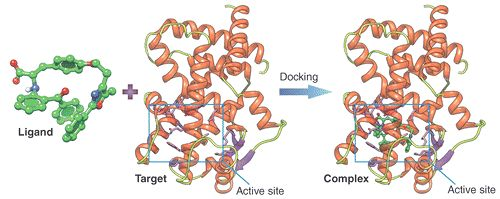
\includegraphics[scale=0.8]{images/chapter1/docking.jpg}
    \caption[Illustrazione grafica del complesso proteina-ligando.]{Illustrazione grafica del complesso proteina-ligando. Sulla sinistra il ligando, al centro la proteina (il riquadro mette in evidenza il sito attivo), a destra la conformazione proteina-ligando a seguito del docking. Fonte: \cite{liao_molecular_2013}}
    \label{fig:molecular_docking}
\end{figure}

In base ai tipi di ligando, il docking può essere classificato come
\begin{itemize}
    \item \textbf{Proteina-ligando}: rappresenta la casistica più semplice dello spettro di complessità e ci sono molti programmi disponibili che funzionano particolarmente bene nel predire le molecole che possono potenzialmente inibire le proteine. 
    A sua volta, il docking proteina-ligando può essere classificato nel modo seguente: 
    \begin{itemize}
        \item[◦] \textbf{Rigid-body docking}, in cui sia il recettore che il ligando sono trattati come rigidi; 
        \item[◦] \textbf{Flexible ligand docking}, in cui il recettore è tenuto rigido, ma il ligando è trattato come flessibile. E' il modello  utilizzato comunemente dagli algoritmi di docking;
        \item[◦] \textbf{Flexible docking}, in cui si considera sia la flessibilità del recettore che del ligando \cite{roy_chapter_2015}.
    \end{itemize}
    \item \textbf{Proteina-acido nucleico}: riguarda processi biologici essenziali, tra cui la replicazione del DNA, la trascrizione dell'RNA, etc. Tuttavia, la determinazione sperimentale della maggior parte delle strutture complesse proteina-acido nucleico con metodi ad alta risoluzione è un processo noioso e difficile.
    \item \textbf{Proteina-proteina}: è in genere molto più complesso. Il motivo è dato dal fatto che le proteine sono flessibili e il loro spazio conformazionale è piuttosto vasto.
\end{itemize}

E' importante sottolineare che le prestazioni del docking dipendono dall'algoritmo di ricerca. Inolte, al fine di evitare fonti di incomprensione od ambiguità, occorre fare una breve premessa sulla terminologia tecnica.


Distinguiamo tra energia di legame e affinità di legame.
L'affinità di legame è un termine usato per trovare l'efficienza del complesso ligando-recettore valutando le interazioni presenti nel complesso attraverso funzioni di scoring, campo di forza e metodi statistici.
L'energia libera di legame o \textit{binding energy} è la somma di tutte le interazioni intermolecolari presenti tra il ligando ed il recettore e può essere utilizzata come una stima di affinità di legame.

L'energia rilasciata a causa della formazione del legame, o meglio, dell'interazione del ligando e della proteina è definita sotto forma di "binding energy" o energia di legame. L'energia libera della reazione favorevole è negativa. Minore è l'energia di legame, migliore è il legame del ligando e della proteina, più il complesso sarà stabile.

\subsection{Breve storia del docking molecolare}
Il legame di una proteina ai ligandi ha una notevole rilevanza nel moderno processo di drug discovery\footnote{Con il termine \textit{drug discovery} s'intende il processo attraverso il quale vengono scoperti nuovi farmaci candidati.}, per tal motivo il docking molecolare è una tecnica ampiamente utilizzata dall'inizio degli anni '80.
Il docking molecolare è stato descritto per la prima volta nel 1982 dallo scienziato americano Tack Kuntz e da allora è diventato l'idea centrale nello \textit{structure-based virtual screening}.
In tempi moderni, la biologia strutturale si sta espandendo giorno dopo giorno, al punto che viene utilizzata da una serie di tecniche computazionali avanzate come l'\textit{high-throughput virtual screening} (vHTS) \cite{noauthor_chapter_nodate,naqvi_advancements_nodate}.
Tuttavia, esistono anche alcune limitazioni delle attuali tecniche di docking, tra cui la complessità, la flessibilità dei ligandi e delle proteine, ecc. \cite{naqvi_advancements_nodate}


\subsection{Passi elementari del docking}
Fondamentalmente, il docking è un processo in tre fasi indipendentemente dal software e dagli algoritmi di docking. 
Il primo passo è la \textbf{preparazione dei ligandi}. In questo processo, tutte le strutture duplicate devono essere rimosse e i parametri per i rispettivi ligandi devono essere impostati nella piattaforma software funzionante \cite{roy_chapter_2015}.

\begin{figure}[H]
    \centering
    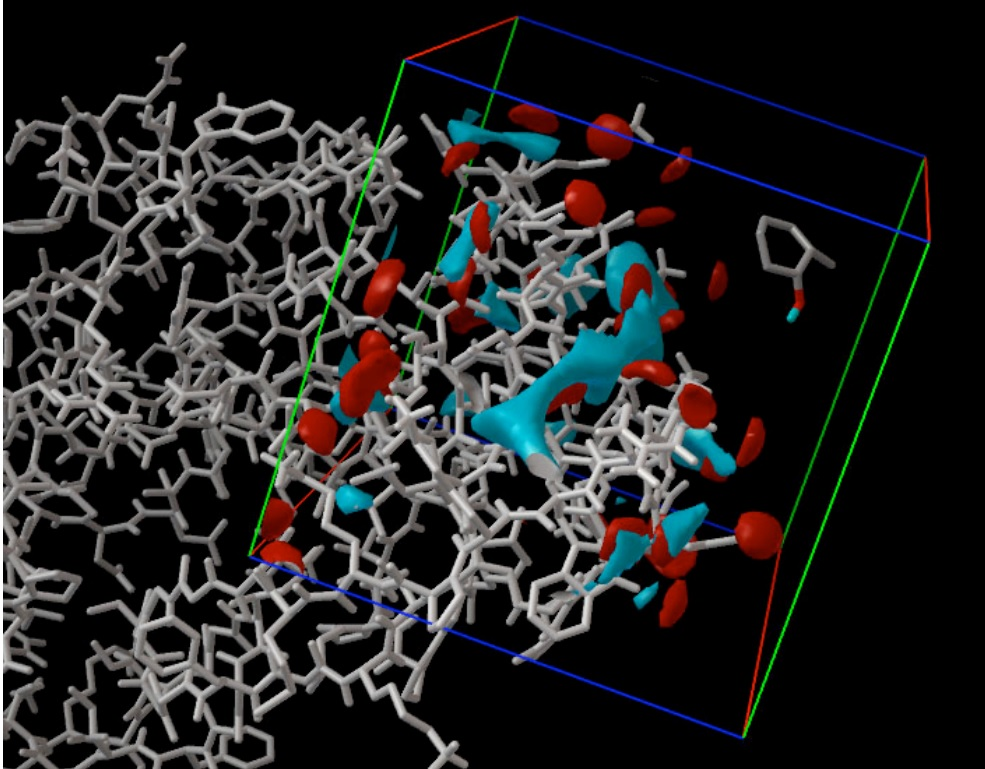
\includegraphics[scale=0.5]{images/chapter1/gridbox.jpg}
    \caption[Rappresentazione visiva di una gridbox in AutoDockTools]{Rappresentazione visiva di una gridbox all'interno di AutoDockTools. La gridbox è rappresentata da un cubo dai lati colorati di rosso, verde e blu. In grigio la struttura proteica, in azzurro è rappresentato il ligando ed in rosso le collisioni tra le strutture. Fonte: \cite{eberhardt_autodock_nodate}}
    \label{fig:gridbox}
\end{figure}

Il secondo passo è la \textbf{preparazione della proteina}: 
\begin{itemize}
    \item è necessario aggiungere atomi di idrogeno, seguito dalla rimozione delle molecole d'acqua tranne nel sito attivo;
    \item la proteina dovrebbe essere regolata correggendo eventuali errori gravi come residui incompleti vicino al sito attivo;
    \item le cariche e i tipi di atomi per qualsiasi atomo di metallo dovrebbero essere impostati correttamente, se necessario;
    \item se ci sono legami con ioni metallici, i legami dovrebbero essere cancellati, quindi aggiustando le cariche formali degli atomi che erano attaccati al metallo, così come il metallo stesso. 
\end{itemize}
La molecola proteica risultante costituisce il recettore pronto per il docking \cite{roy_chapter_2015}.

Dopo aver verificato che la proteina e i ligandi siano nella forma corretta per il docking, in alcuni casi si passa alla \textbf{generazione della gridbox} per ogni recettore. La \textit{gridbox}\footnote{La posizione della gridbox definisce la regione della proteina in cui verrà eseguito il docking. Qualsiasi regione al di fuori della gridbox non verrà esplorata durante il docking.} è generalmente generata al baricentro del ligando legato al sito attivo del recettore. 
In altri casi, vengono identificate cavità o sacche attive della proteina in cui fissare il ligando \cite{roy_chapter_2015}.

A questo punto del processo, viene effettuato il \textbf{docking proteina-ligando}, che consiste nella ricerca accurata del corretto orientamento e della corretta conformazione di un ligando all'interno di una cavità della proteina e nella valutazione di tali pose attraverso l'applicazione della funzione di scoring, la quale restituisce una misura di energia della posa, indicata con il termine \textit{affinità} \cite{roy_chapter_2015}.

\begin{figure}[H]
    \centering
    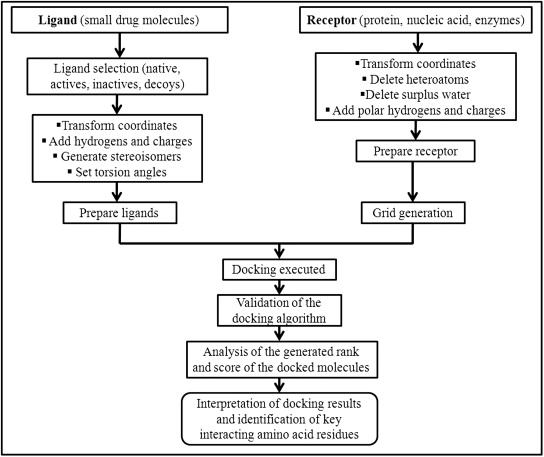
\includegraphics[scale=0.9]{images/chapter1/docking_steps.jpg}
    \caption[Schema riassuntivo dei passi del docking.]{Schema riassuntivo dei passi del docking. A sinistra la preparazione dei ligandi, a destra la preparazione delle proteine. Al centro è sintetizzato il processo di docking. Fonte: \cite{roy_chapter_2015}}
    \label{fig:docking_steps}
\end{figure}

Per ogni particolare posa viene contato il numero di interazioni intermolecolari favorevoli come legami idrogeno e contatti idrofobici. 
Al fine di riconoscere la posa energeticamente migliore, ogni posa viene valutata in base alla sua compatibilità con il target in termini di forma e proprietà e viene generato il punteggio corrispondente. Un buon punteggio per un dato ligando significa che è potenzialmente un buon legante \cite{roy_chapter_2015}.

Un determinato numero di pose del ligando viene salvato per ogni conformazione del ligando. Dopodichè viene effettuato il \textbf{ranking}, ovvero il processo di classificazione dei ligandi in cui le pose determinate e salvate per ciascuna conformazione del composto vengono ordinate in base ai rispettivi punteggi (cioè, le loro affinità previste).  Questo elenco ordinato viene quindi utilizzato per ulteriori sintesi e indagini biologiche solo per quei composti che si prevede siano più attivi \cite{roy_chapter_2015}.


\subsection{Requisiti essenziali per il docking} \label{requirements}
I requisiti essenziali per poter effettuare il docking molecolare riguardano la struttura molecolare del recettore così come le strutture di un insieme di ligandi di interesse.

La struttura del recettore può essere determinata mediante tecniche sperimentali come la cristallografia a raggi X o la spettrografia NMR. Tale struttura può essere facilmente scaricata dal \textit{Protein Data Bank}\footnote{Il \textit{Protein Data Bank} (PDB) è un archivio per dati di struttura in 3-D di proteine e acidi nucleici. Finora sono state depositate nel database PDB (http://www.rcsb.org) più di 140.000 strutture molecolari tridimensionali di diverse biomacromolecole tra cui molte proteine e complessi proteina-ligando \cite{naqvi_advancements_nodate}.} \cite{roy_chapter_2015}. 

La qualità della struttura del recettore gioca un ruolo cruciale nel successo del docking computazionale. In generale, maggiore è la risoluzione della struttura cristallina impiegata, migliori sono i risultati di docking osservati.

Un altro criterio importante per esaminare la qualità di una struttura recettoriale è il fattore Debye Waller (DWF)\footnote{Il fattore di Debye-Waller, noto anche come fattore B o fattore di temperatura, descrive la variazione dell'intensità di scattering (sia di raggi X, sia di neutroni) dovuta al moto termico degli atomi o al disordine del cristallo.}.

Al contrario, se la struttura cristallina a raggi X della proteina non è disponibile, si può optare per la predizione della struttura. In tal caso, le tecniche più comunemente applicate sono il \textit{“threading”} e l'\textit{“homology modeling”}. Nel caso del threading, viene effettuata una stima se una determinata sequenza di amminoacidi è compatibile con uno dei ligandi in un database.
D'altra parte, l'homology modeling si basa su una correlazione o omologia tra la sequenza della proteina-obiettivo ed almeno una struttura nota. \cite{roy_chapter_2015}

Le strutture dei ligandi di interesse sono ricavate da PubChem\footnote{PubChem è un database di molecole chimiche, gestito dal centro nazionale per l'Informazione biotecnologica statunitense (NCBI), parte della biblioteca nazionale di medicina (NLM) dell'istituto nazionale della sanità americano (NIH).} oppure dalle banche dati dedicate, messe a disposizione dalla Commissione Europea, come ad esempio l'EU Pesticides Database.


\section{Implementazione del docking molecolare} \label{implementazione_docking}
Come anticipato nella Sezione \ref{docking_molecolare}, il docking molecolare prevede una fase di campionamento dello spazio conformazionale del complesso proteina-ligando e una fase di valutazione della migliore conformazione trovata. 
Per poter esaminare lo spazio conformazionale, è necessario applicare un algoritmo di campionamento come ad esempio il campionamento di Monte Carlo. Le conformazioni campionate vengono valutate attraverso una funzione di scoring, che a sua volta applica un algoritmo di ottimizzazione come l'algoritmo di Broyden-Fletcher-Goldfarb-Shanno.
In questa sezione sono descritti il concetto di funzione di scoring e gli algoritmi che costituiscono il docking molecolare.

\subsection{Algoritmo di campionamento dello spazio conformazionale}
Lo spazio conformazionale del ligando viene esplorato utilizzando il \textbf{campionamento di Monte Carlo}; tendenzialmente le catene sono eseguite in parallelo utilizzando i threads della CPU. Il numero degli steps per le catene di Monte Carlo sono calcolati sulla base del numero degli atomi mobili e sul numero dei gradi di libertà all'interno del ligando. 

Ad ogni passo della catena di Monte Carlo, il ligando è modificato selezionando casualmente una delle seguenti operazioni: traslazione casuale, rotazione casuale dell'intera molecolare, o selezionando gli angoli di torsione del ligando in maniera casuale. 

Il processo di Monte Carlo prevede il ripristino casuale degli angoli di torsione con una probabilità maggiore rispetto alle altre mutazione. Dopo la mutazione, è effettuata una minimizzazione dell'energia approssimativa,  secondo una certa funzione di scoring, che può essere empirica (non-CNN) o CNN. 

\subsection{Funzioni di scoring}
Le funzioni di scoring forniscono una relazione dallo spazio conformazionale del ligando e del recettore all'insieme dei numeri reali in modo che le pose possano essere classificate. 
La forma e la parametrizzazione delle funzioni di scoring varia ampiamente tra le implementazioni \cite{mcnutt_gnina_2021}.

Tipicamente, le funzioni di scoring sono raggruppate in quattro categorie:
\begin{itemize}
    \item \textbf{basate sulla conoscenza}, derivate utilizzando statistiche per le frequenze di contatto interatomiche osservate, le distanze od entrambe, in un ampio database di strutture cristalline di complessi proteina-ligando. Le funzioni di scoring basate sulla conoscenza possono essere influenzate dalle caratteristiche presenti nei loro set di formazione sebbene i calcoli dei punteggi siano rapidi al momento del test. Richiedono un ampio database di strutture conosciute e possono essere difficili da interpretare quando si cerca di comprendere un punteggio \cite{mcnutt_gnina_2021, koes_lessons_2013}; 
    
    \item \textbf{basate sul campo di forza}, cercano di quantificare le effettive forze molecolari che esistono tra una proteina e una piccola molecola. Le interazioni di Van der Waals, le interazioni elettrostatiche e le interazioni di legame idrogeno sono componenti comuni delle funzioni di scoring basate sul campo di forza. Questi termini sono idealmente parametrizzati dai primi principi. Le funzioni di scoring del campo di forza sono spesso progettate per l'uso nelle simulazioni di dinamica molecolare. Tuttavia, l'accuratezza di tali funzioni basate sulla fisica è limitata dalla loro complessità e dalle ipotesi che poniamo sulle forze fondamentali che dettano le interazioni tra le molecole, sebbene la comprensione di queste forze sia in continuo aumento \cite{mcnutt_gnina_2021, koes_lessons_2013}; 
    
    \item \textbf{empiriche}, affrontano i limiti delle funzioni di punteggio basate sulla fisica utilizzando una combinazione di termini energetici selezionati manualmente. Invece di assegnare a ciascun termine energetico una ponderazione identica, i pesi di ciascun termine sono determinati tramite un adattamento ai dati sperimentali. Possono avere termini simili alle funzioni di scoring basate sul campo di forza e possono anche contenere termini più complessi ed euristici, come le interazioni idrofobiche. Come le funzioni di scoring basate sulla conoscenza, le prestazioni delle funzioni di scoring empiriche dipendono e migliorano con la quantità e la qualità dei dati di addestramento. Gran parte del software di docking utilizza funzioni di punteggio empirico, tra cui AutoDock Vina \cite{mcnutt_gnina_2021, koes_lessons_2013};
    \item \textbf{CNN}, prende in input una rappresentazione 3D di un complesso proteina-ligando ed apprende automaticamente le caratteristiche chiave delle interazioni correlate al legame. Le funzioni di scoring CNN possono essere addestrate ed ottimizzate per discriminare tra pose corrette e scorrette e leganti noti e non leganti \cite{mcnutt_gnina_2021}.
\end{itemize}

\subsection{Algoritmo di ottimizzazione} \label{bfgs}
Nell'implementazione della funzione di scoring Vina, utilizzata dai software che saranno presentati nel prossimo capitolo, viene utilizzato il metodo \textbf{Broyden-Fletcher-Goldfarb-Shanno} (BFGS) per l'ottimizzazione locale, che è un metodo quasi-Newton efficiente. 
BFGS è un metodo iterativo per risolvere problemi di ottimizzazione non lineare non vincolata e, come altri metodi di ottimizzazione quasi-Newton, utilizza non solo il valore della funzione di scoring ma anche il suo gradiente, ovvero le derivate della funzione di scoring rispetto ai suoi argomenti. Gli argomenti, nel nostro caso, sono la posizione e l'orientamento del ligando, così come i valori delle torsioni per i legami ruotabili attivi nel ligando e gli eventuali residui flessibili \cite{trott_autodock_2009}.

Sebbene la valutazione del gradiente oltre al valore della funzione di scoring stessa possa richiedere più tempo, il suo utilizzo può accelerare notevolmente l'ottimizzazione. Il numero di iterazioni in un'esecuzione è determinato in modo adattivo, in base all'apparente complessità del problema, e vengono eseguite più esecuzioni a partire da conformazioni casuali. Queste esecuzioni possono essere eseguite contemporaneamente, utilizzando il multithreading. Ciò consente di sfruttare il parallelismo hardware a memoria condivisa, come le ormai onnipresenti CPU multicore. L'algoritmo di ottimizzazione mantiene una serie di diversi minimi significativi trovati che vengono quindi combinati da esecuzioni separate e utilizzati durante la fase di perfezionamento della struttura e clustering \cite{trott_autodock_2009}.

L'analisi di clustering è il modo migliore per determinare se la simulazione ha ispezionato adeguatamente lo spazio conformazionale disponibile \cite{forli_computational_2016}. Questa consiste nell'eseguire più simulazioni di docking e confermare che la migliore conformazione viene trovata più volte.

\section{Virtual Screening}
Nella modellazione di farmaci basata sulla struttura, ottenere il modello più accurato ed efficiente di complesso ligando-recettore è un passaggio cruciale ed è un punto di partenza adatto per ulteriori valutazioni per testare nuovi composti o possibili farmaci candidati \cite{menchaca_past_2020}.
 
Il \textit{virtual screening} o il \textit{virtual high-throughput screening} (vHTS) è una potente tecnica computazionale utilizzata nel processo di scoperta di farmaci per identificare piccoli composti bioattivi, mediante la ricerca in alcune librerie chimiche, che possono legarsi efficacemente ad un particolare farmaco target, e che possono essere usati come riferimento o \textit{lead compounds}\footnote{Lead compounds, composti guida} \cite{naqvi_advancements_nodate}.

L'accuratezza di questa tecnica è notevolmente migliorata negli ultimi anni e ciò ha permesso di far ormai parte ad una serie di tecniche computazionali che consentono ai ricercatori di ridurre una vasta libreria di composti ad una dimensione più conveniente. Queste tecniche consentono la valutazione di ampie librerie di composti chimici rispetto ad un target biologico ma soprattutto uno screening rapido ed efficace \cite{naqvi_advancements_nodate}.

Gli approcci VS sono stati vigorosamente implementati dalle industrie farmaceutiche con l'intento di ottenere il maggior numero possibile di potenziali composti, con la speranza di una maggiore possibilità di trovare risultati dall'ampio pool disponibile di librerie chimiche. Molti esempi di successo sono stati dimostrati di recente nell'identificazione di lead compounds \cite{roy_chapter_2015}.

Tuttavia, l'approccio VS dipende fortemente dalla quantità e qualità dei dati disponibili e dalla capacità di predizione dell'algoritmo sottostante. Di conseguenza, non esiste una linea guida o un flusso di lavoro universale per queste tecniche, per cui il ricercatore deve applicare la sua conoscenza ed esperienza computazionale per trovare il farmaco candidato attivo tra grandi database di farmaci e librerie chimiche, applicando i migliori strumenti possibili secondo le sue esigenze \cite{roy_chapter_2015}.

Inoltre, poiché ogni target biologico è unico, non sembra esserci un metodo universale per eseguire questi studi.

\begin{figure}[H]
    \centering
    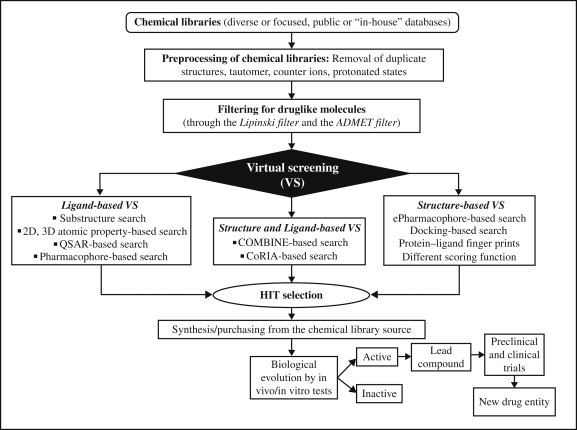
\includegraphics[scale=0.9]{images/chapter1/virtual_screening.jpg}
    \caption[Passi nell'applicazione del virtual screening.]{Passi nell'applicazione del virtual screening. A seguito di una fase di preprocessing, vengono illustrati differenti approcci di virtual screening ed infine vengono trattati possibili hit in vivo/in vitro per classificare il sito come attivo o inattivo. Fonte: \cite{roy_chapter_2015}}
    \label{fig:virtual_screening}
\end{figure}

Sebbene non si possano ignorare le restrizioni intrinseche del VS, rimane una delle migliori opzioni possibili per esplorare un ampio spazio chimico, in termini di efficacia dei costi e impegno di tempo e materiale necessario. 
Con lo sviluppo di nuove metodologie di docking, tecniche di screening basate su ligandi e sistemi di \textit{machine learning}, le tecniche VS sono in grado di fornire \textit{hit prediction rate} migliori e, senza dubbio, svolgeranno un ruolo di primo piano nella progettazione di farmaci nel prossimo futuro sia come approccio complementare all'HTS o come approccio autonomo \cite{roy_chapter_2015}.

\section{Applicazione del docking computazionale} 
Nell'ambito della valutazione dei rischi, il docking computazionale ha un ruolo molto importante poiché, attraverso la potenza di calcolo delle macchine moderne e la quantità di strutture molecolari tridimensionali ottenute e memorizzate in grandi database, è possibile evitare e limitare gli esperimenti \textit{in vitro}, a favore dell'analisi delle interazioni \textit{in silico} ed a sostegno delle nuove metodologie di approccio (NAM), riconosciute dall'Agenzia statunitense per la protezione dell'ambiente (US EPA) \cite{us_epa_alternative_2017, scitovation_what_2021}.

La nascita del docking computazionale ha dato vita ad analisi di valutazione dei rischi condotte attraverso approcci computazionali efficaci, permettendo quindi di verificare e spiegare l'esistenza di una correlazione tra la tossicità di particolari pesticidi e la perdita di colonie di api mellifere, evitando il ricorso a tecniche di analisi \textit{in vitro}.
\subsection{Correlazione tra pesticidi ed api} \label{Apis mellifera}
Un esempio di applicazione del docking computazionale è sicuramente la valutazione dei rischi delle api mellifere esposte ai pesticidi comunemente utilizzati nell'agricoltura moderna.
La tematica è stata centrale nel lavoro di tirocinio interno presso il Consiglio Nazionale delle Ricerche (CNR), seguiti dal Prof. Angelo Ciaramella e dal Dott. Ferdinando Febbraio, svolto assieme al collega Alfredo Mungari, anch'egli laureando in Informatica Parthenope. 

L'attività svolta è partita da un'analisi di valutazione dei rischi,
condotta dal Dott. Ferdinando Febbraio e dalla Dott.ssa Mónica del Águila, biologa ambientale specializzata in Ecotossicologia, riguardo una correlazione tra pesticidi e le proteine da api mellifere con struttura 3D nota. Questo studio ha portato alla realizzazione di un software di supporto per l'automatizzazione di processi inerenti al docking computazionale.

\subsubsection{L'importanza degli impollinatori}
L'impollinazione delle api offre un'ampia varietà di benefici all'umanità, contribuendo alla trasformazione degli alimenti, alle materie prime, ai medicinali, alle fibre, ai valori sociali e culturali e al mantenimento della biodiversità e della protezione ambientale.

In botanica, l’impollinazione è definita come quel processo che consiste nel trasporto dei pollini dalla parte maschile e quella femminile dell’apparato riproduttivo delle piante, all'interno dello stesso fiore (self-pollination) o tra le piante (cross-pollination). 

Attualmente, il 5-8\% di tutta la produzione agricola globale andrebbe persa senza i servizi di impollinazione forniti dalle api, rendendo necessari cambiamenti nella dieta umana e l'espansione dei terreni agricoli per risolvere le carenze nella produzione agricola \cite{khalifa_overview_2021}. 

La riduzione della popolazione delle api ha destato una forte preoccupazione negli ultimi anni poiché rappresenta tutt'oggi un problema di globale importanza.
\cite{di_prisco_neonicotinoid_2013,li_neonicotinoid_2015}.

La perdita di impollinatori, i quali hanno un ruolo fondamentale nella produzione agricola mondiale, impatta indirettamente anche sul mercato globale, specie per i paesi che basano una buona parte della propria economia sui prodotti in cui interviene, in qualche maniera, l'impollinazione da insetti, ed in particolare delle api. In relazione ai loro orientamenti agricoli, alcune regioni sono apparse più vulnerabili come il Medio Oriente asiatico, l'Asia centrale, l'Asia orientale ed i paesi non appartenenti all'Unione Europea, principalmente importatori \cite{gallai_economic_2009}. Tuttavia, questo fenomeno colpisce quasi tutte le regioni del pianeta: questo ne motiva l'importanza e la drammaticità.

L'esposizione delle api a numerosi fattori di stress e l'impatto degli agenti patogeni, enfatizzato dall'esposizione a particolari pesticidi, ad esempio i neonicotinoidi\footnote{I neonicotinoidi sono insetticidi sistemici che vengono trasferiti nel polline e nel nettare di molte colture impollinate, è uno dei principali cofattori associati alla perdita di api.}, spiegano il collasso delle colonie, spesso associate ad alti livelli di infezione. 

I neonicotinoidi furono registrati per la prima volta agli anni '90 e nel 2010 rappresentarono un terzo del mercato globale degli insetticidi. La scarsa regolamentazione vigente fu la causa della loro diffusione, la quale fallì nel riconoscere i potenziali effetti ecologici ed ambientali del loro utilizzo \cite{sgolastra_bees_2020}. 

\subsubsection{CCD: Colony Collapse Disorder}

L'esposizione a prodotti chimici per l'agricoltura come fungicidi, insetticidi e pesticidi, causa contaminazione, tossicità e diminuzione della qualità e quantità dei nutrienti nel polline e nel nettare, portando a una cattiva salute delle colonie e quindi minacciando la sopravvivenza delle api (CCD\footnote{Il \textit{disturbo da collasso della colonia} (CCD) è un fenomeno per cui si verificano perdite rapide e inspiegabili di api da lavoro adulte in colonie di api gestite (ad esempio, colonie di api mellifere negli Stati Uniti), con il risultato che rimangono solo la regina e poche api che allattano.}, Colony Collapse Disorder).\cite{khalifa_overview_2021}.

\begin{figure}[H]
    \centering
    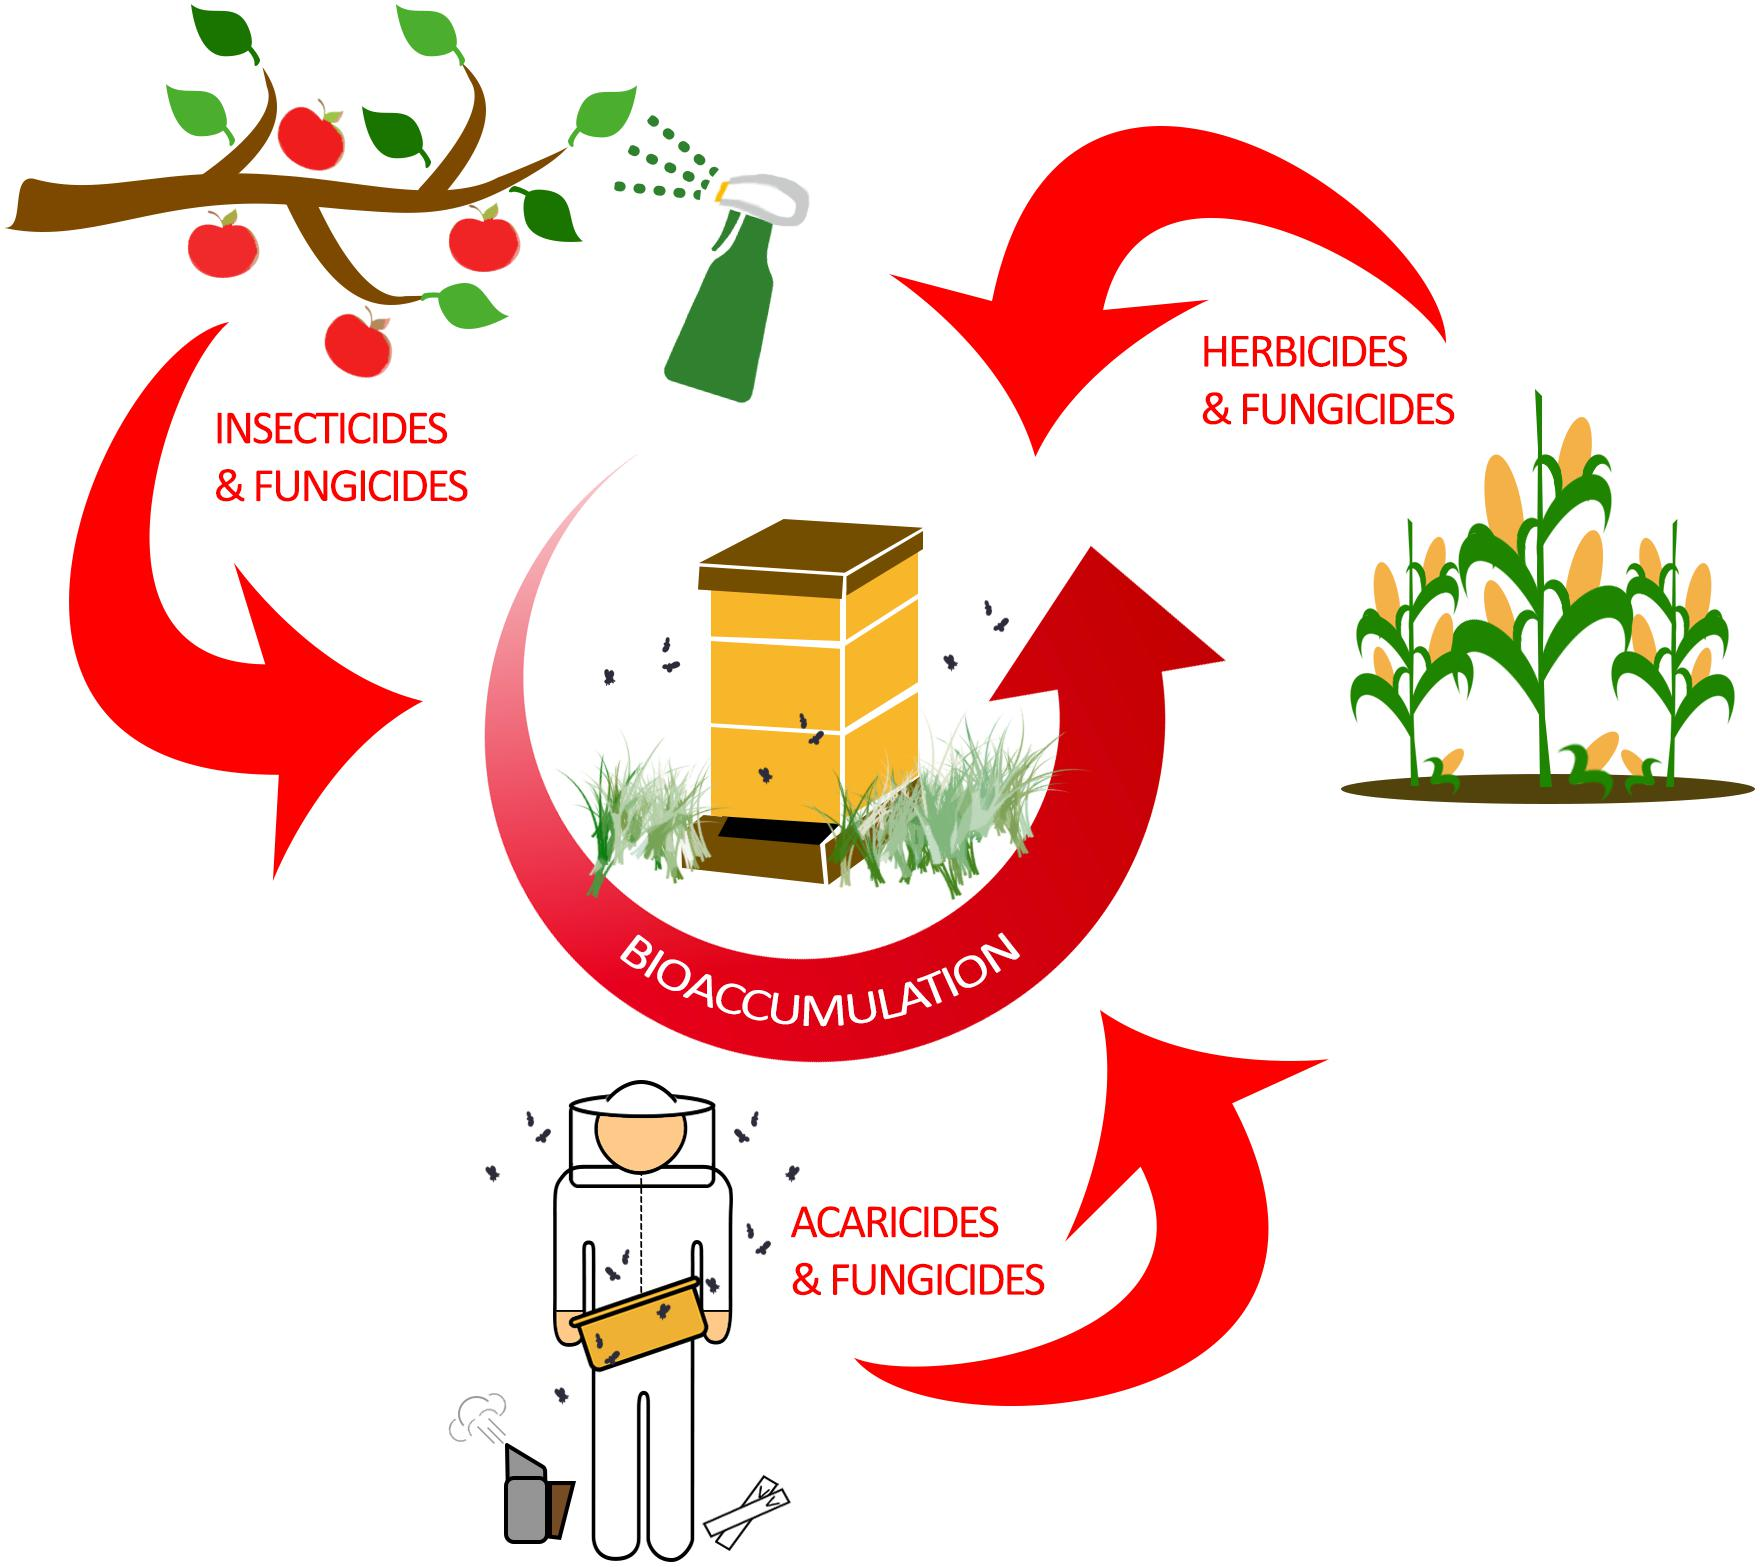
\includegraphics[scale=1.2]{images/chapter1/bioaccumulation.jpg}
    \caption[Bioaccumulo di pesticidi in una colonia di api mellifere.]{Bioaccumulo di pesticidi in una colonia di api mellifere. Le api mellifere sono esposte a un'ampia varietà di pesticidi attraverso pratiche agricole e l'apicoltura moderna. Mentre le api mellifere si nutrono di nettare e polline, sono accidentalmente esposte ai pesticidi che si accumulano nell'alveare trasferendo fisicamente le fonti di cibo contaminate alle api non esposte. Tuttavia, le api mellifere possono anche essere intenzionalmente esposte ad acaricidi e fungicidi dagli apicoltori nel tentativo di controllare il carico di acari e le malattie fungine nell'alveare. Fonte: \cite{chmiel_understanding_2020}}
    \label{fig:bioaccumulation}
\end{figure}

Poiché la tossicità è il principale fattore di rischio, le combinazioni sinergiche di fungicidi con particolari pesticidi sono fonte di grande preoccupazione poiché tale tossicità, già intrinsecamente elevata nei singoli composti, viene potenziata spaventosamente quando combinati insieme. 

Per questo motivo, l'esposizione ai pesticidi ad alte dosi è un fattore causale notevole coinvolto nel calo della popolazione delle api mellifere; tuttavia, l'esposizione ai pesticidi subletali presenta minacce non visibili per le api mellifere, portando a neurotossicità, immunodeficienza, cambiamenti comportamentali e disturbi cronici, oltre ad inficiare negativamente sulla riproduzione \cite{chmiel_understanding_2020}. 

\chapter{Tecnologie e Piattaforme}

\vskip 1cm
\textit{In questo capitolo vengono discussi in maniera approfondita i concetti alla base delle reti neurali convoluzionali ed il funzionamento dei software di docking considerati. Vengono discusse le tecnologie e piattaforme, software ed hardware, utilizzate al fine di produrre l'applicazione proposta nell'elaborato. }

\vskip 1cm
\section{Breve introduzione al Deep Learning}
Gli approcci computazionali per il processo di drug discovery possono ridurre i tempi ed i costi associati ai test sperimentali e consentire lo screening di nuovi composti. I metodi di progettazione dei farmaci basati sulla struttura molecolare si basano su funzioni di scoring per classificare e prevedere le affinità e le pose. 
La quantità in \textbf{continua espansione} di dati strutturali consente l'uso di tecniche di \textit{deep learning} per lo scoring del complesso proteina-ligando \cite{ragoza_protein-ligand_2017}.

Il Deep Learning è una sottocategoria del Machine Learning ed indica quella branca dell’Intelligenza Artificiale che fa riferimento agli algoritmi ispirati alla struttura e alla funzione del cervello, chiamati reti neurali artificiali. Queste consistono in modelli di calcolo matematico-informatici basati sul funzionamento delle reti neurali biologiche, ossia modelli costituiti da interconnessioni di informazioni. 

Una rete neurale di fatto si presenta come un sistema “adattivo” in grado di modificare la sua struttura (i nodi e le interconnessioni) basandosi sia su dati esterni sia su informazioni interne che si connettono e passano attraverso la rete neurale durante la fase di apprendimento.

Il Deep Learning si riferisce a reti neurali con molti livelli, che sono in grado di apprendere funzioni altamente complesse, rese pratiche in gran parte dall'aumento della potenza di calcolo fornita dalle moderne schede grafiche \cite{ragoza_protein-ligand_2017}.


\begin{figure}[H]
    \centering
    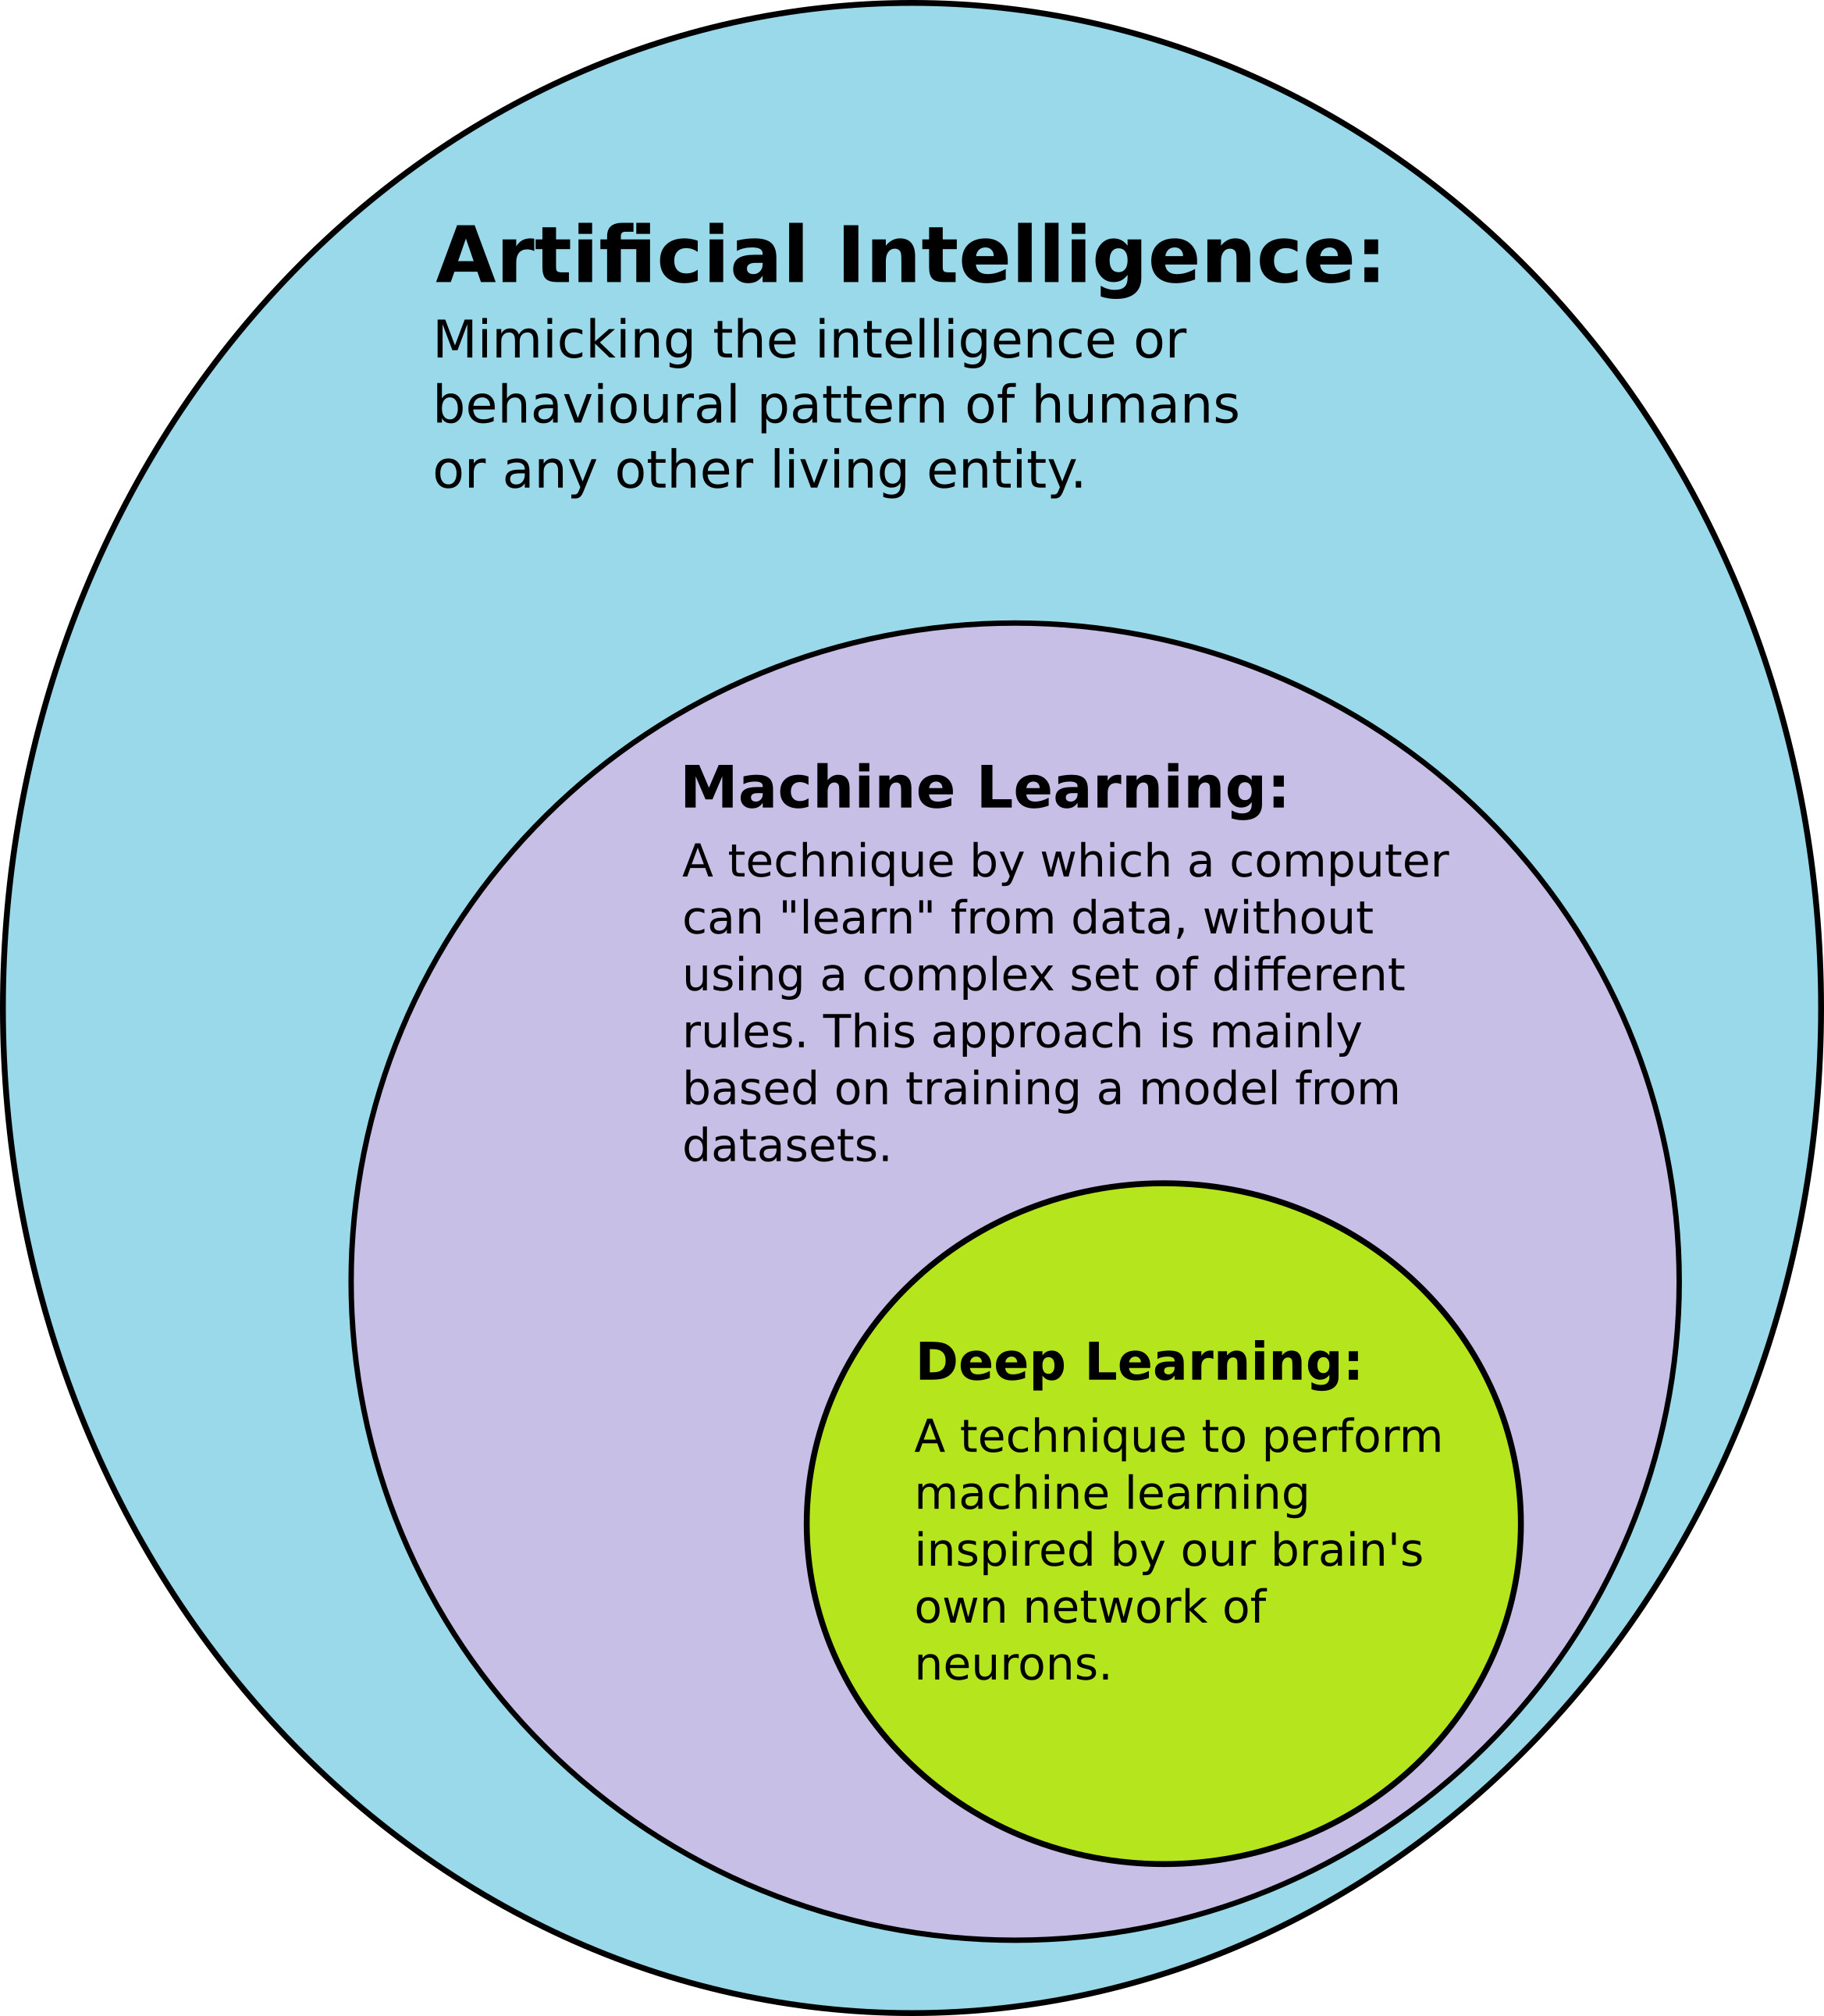
\includegraphics[width=0.5\textwidth]{images/AI-ML-DL.jpg}
    \caption[Relazione tra IA, ML e DL.]{Relazione tra Intelligenza Artificiale, Machine Learning e Deep Learning. Tradotto: l'Intelligenza artificiale mima l'intelligenza od il comportamento di umani o qualsiasi altra entità vivente; il Machine Learning è una tecnica in cui il computer può "imparare" dai dati, senza utilizzare un insieme complesso di regole differenti. Questo approccio è principalmente basato sull'addestramento di un modello dai dati; il Deep Learning è una tecnica per eseguire un approccio di machine learning, ispirata dalla rete di neuroni del nostro del nostro cervello. Fonte: \url{https://en.wikipedia.org/wiki/Deep_learning}}
    \label{fig:ai_ml_dl}
\end{figure}

Una rete di base è costituita da uno strato di input, uno o più strati nascosti e uno strato di output di nodi interconnessi. Ogni nodo nascosto calcola una caratteristica che è una funzione dell'input ponderato che riceve dai nodi del livello precedente. Gli output vengono propagati a ogni livello successivo finché il livello di output non genera una classificazione \cite{ragoza_protein-ligand_2017}.

L'architettura della rete e la scelta della funzione di attivazione per ogni livello determinano il design della rete. I pesi che parametrizzano il modello sono in genere ottimizzati per adattarsi a un determinato set di dati di addestramento per ridurre al minimo l'errore della rete, senza eccedere nell'overfitting\footnote{In statistica e in informatica, si parla di overfitting o sovradattamento quando un modello statistico molto complesso si adatta ai dati osservati perché ha un numero eccessivo di parametri rispetto al numero di osservazioni. } \cite{ragoza_protein-ligand_2017}.

\section{CNN: Convolutional Neural Network}

Le \textit{reti neurali convoluzionali} (CNN) sono un tipo di rete neurale comunemente usata nel riconoscimento delle immagini. Le CNN scompongono gerarchicamente un'immagine in modo che ogni livello della rete impari a riconoscere le caratteristiche di livello superiore mantenendo le loro relazioni spaziali \cite{ragoza_protein-ligand_2017}.

Le applicazioni che richiedono il riconoscimento di oggetti e la visione artificiale, come i veicoli a guida autonoma e le applicazioni di riconoscimento facciale, si basano ampiamente sulle CNN.
Le impressionanti prestazioni delle CNN nell'attività di riconoscimento delle immagini suggeriscono che sono adatte per l'apprendimento da altri tipi di dati spaziali, come le strutture proteina-ligando \cite{ragoza_protein-ligand_2017}. 

\begin{figure}[H]
    \centering
    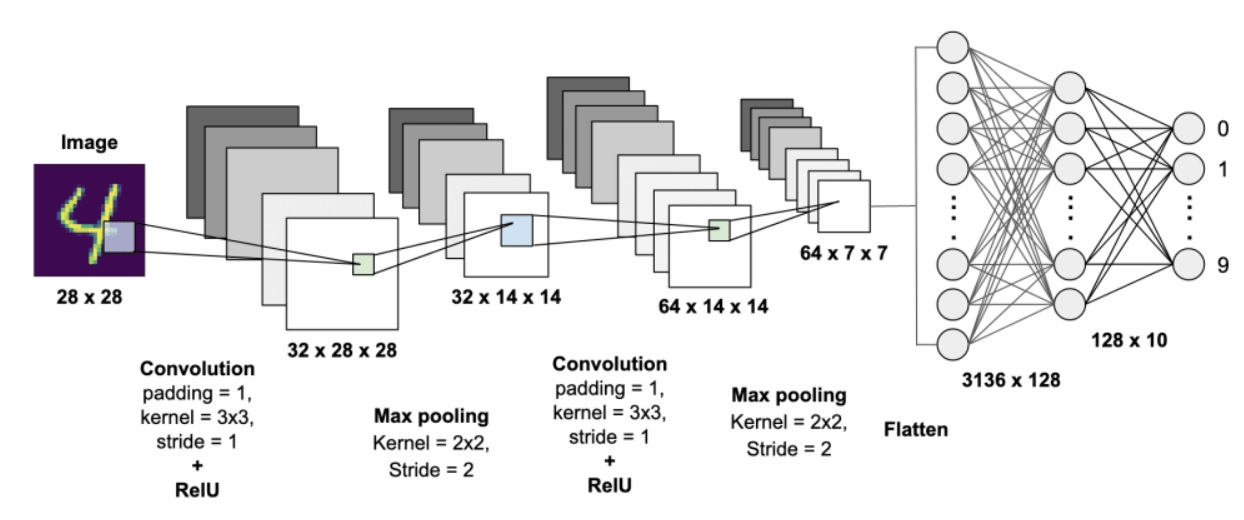
\includegraphics[scale=0.55]{images/convNet.jpg}
    \caption[Esempio di CNN per il riconoscimento di numeri arabi.]{Esempio di rete neurale convoluzionale per il riconoscimento di numeri arabi. A sinistra l'immagine di input, al centro i layer del modello e la relativa funzione di attivazione, a destra la relativa rappresentazione come rete di neuroni. Fonte: \url{https://dev.to/afrozchakure/cnn-in-a-brief-27gg}}
    \label{fig:conv_net}
\end{figure}

L’utilizzo delle CNN per il deep learning è diffuso per via di tre fattori importanti:
\begin{itemize}
    \item eliminano la necessità di estrarre manualmente le \textbf{features} in quanto queste vengono apprese direttamente dalla CNN. Ciò consente l'estrazione di caratteristiche che non sono prontamente codificate in potenziali semplificati, come l'involucro idrofobico o termini dipendenti dalla superficie, così come le caratteristiche che non sono state ancora identificate come rilevanti da alcuna funzione di scoring esistente;
    \item producono risultati di riconoscimento ad alta precisione;
    \item possono essere addestrate nuovamente per nuove attività di riconoscimento, consentendo agli utenti di basarsi sulle reti preesistenti.
\end{itemize}

Le CNN rappresentano una tecnologia chiave in applicazioni come l'imaging biomedico, elaborazione audio, sistemi di guida autonoma e nella generazione di dati sintetici.

% storia delle reti neurali 
\subsection{Storia delle reti neurali convoluzionali}
Il primo modello teorico di un rudimentale neurone artificiale vede la luce nel 1943 grazie ad una coppia di scienziati, Warren Sturgis \textbf{McCulloch} (neurofisiologo) e Walter \textbf{Pitts} (matematico) nella loro pubblicazione \textit{“A logical calculus of the ideas immanent in nervous activity”}. 
I due descrivono un apparato in grado di ricevere \(n\) dati binari in ingresso in ognuno dei suoi elementi, a cui segue un singolo dato in uscita per ciascuno. Si dimostrò essere un "combinatore lineare a soglia", in grado di calcolare semplici funzioni booleane \cite{ai4b_reti_neurali, ia_reti_neurali}.

Nel 1949 lo psicologo canadese Donald Olding \textbf{Hebb} ipotizza la possibilità di istruire le macchine con un apprendimento che emuli quello alla base dell’intelligenza umana \cite{ia_reti_neurali}.

Nel 1958 viene proposta da Frank \textbf{Rosenblatt} (psicologo e computer scientist americano) la prima rete neurale: \textbf{Perceptron}, che possiede uno strato di nodi (neuroni artificiali) di input e un nodo di output.
I pesi sinaptici (un peso indica la forza di una connessione fra due nodi) sono dinamici, permettendo alla macchina di apprendere, in un modo sommariamente simile, anche se molto più elementare, a quello delle reti neurali biologiche. Il modello è feedforward: gli impulsi si propagano in un’unica direzione, in avanti. Tuttavia, il suo campo di applicazione è molto limitato \cite{ia_reti_neurali, ai4b_reti_neurali}.

Le teorie di Rosenblatt scaldano la comunità scientifica per oltre un decennio ma nel 1969 Marvin \textbf{Minsky} e Seymour \textbf{Papert} ne dimostrano i forti limiti: Perceptron risulta essere infatti una rete neurale poco potente, incapace di calcolare la funzione “or esclusivo” (XOR) \cite{ai4b_reti_neurali, camastra_machine_2015}.

Paul \textbf{Werbos}, nel 1974, descrive nella sua tesi di dottorato come impostare l’apprendimento di un MLP \cite{ia_reti_neurali}.

Nel 1986 David \textbf{Rumelhart} introduce il terzo strato delle reti neurali (hidden layers), che caratterizza il \textbf{Multi-Layer Perceptron} (MLP): al suo interno, fra i nodi di input e quello di output si trova uno strato hidden, dove avviene l’elaborazione delle informazioni provenienti dallo strato di input, che poi vengono inviate al nodo di output. È una rete feedforward non lineare: le connessioni in ingresso e in uscita da ogni singolo nodo sono multiple. A merito di tale architettura, il MLP può computare qualsiasi funzione. Inoltre, sempre nel 1986, David \textbf{Rumelhart}, Geoffrey \textbf{Hinton} (premio Turing) e Ronald \textbf{Williams} elaborano il celebre \textbf{Error Back-Propagation}, ancora oggi utilizzato, presentato nel libro \textit{"Parallel Distributed Processing"} \cite{ai4b_reti_neurali, ia_reti_neurali, camastra_machine_2015}.

L’EBP permette di perfezionare in stadi successivi l’apprendimento automatico di una rete neurale. Si implementa modificando i pesi delle connessioni fra nodi che non producono l’output ottimale, finché non si ottiene quest’ultimo \cite{ia_reti_neurali}.

Dalla fine degli anni ’80, con l’arrivo sul mercato di nuovi potenti processori e avanzati chip in grado di supportare applicazioni intensive come quelle delle analisi e delle simulazioni, il percorso di avanzamento tecnologico dell’hardware non si è più arrestato \cite{ai4b_reti_neurali}. 

Allo stato attuale dell'arte, nei laboratori di ricerca si sta lavorando ai \textbf{chip neuromorfici} (che imitano il funzionamento del cervello umano) e a quelli per il \textbf{quantum computing} \cite{ai4b_reti_neurali}{}.

% Apprendimento delle feature, layer e classificazione
\subsection{Apprendimento delle feature, layer e classificazione} \label{cnn}
Analogamente ad altre reti neurali, una CNN è costituita da un layer di input, un layer di output e tanti layer intermedi nascosti.

\begin{figure}[H]
    \centering
    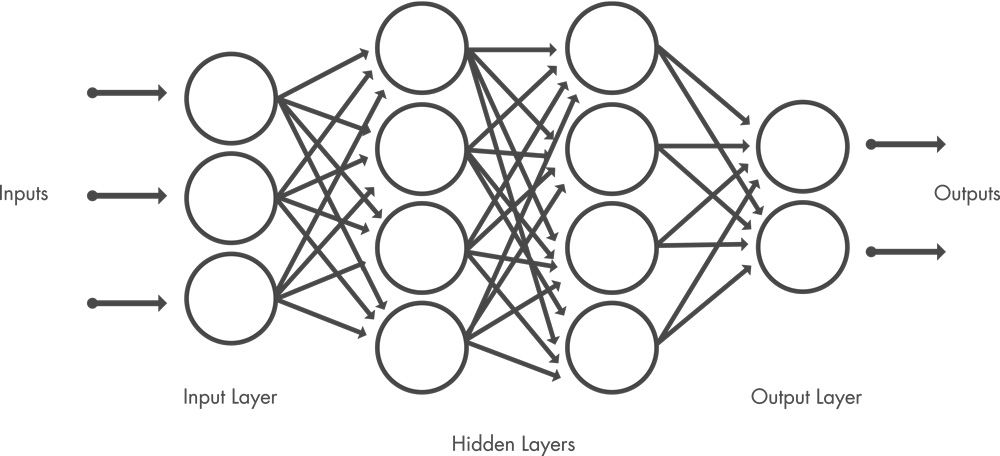
\includegraphics[scale=0.34]{images/cnn_layers.jpg}
    \caption[Esempio di rete neurale per il deep learning.]{Esempio di rete neurale \textit{fully connected} per il deep learning. La figura mostra lo strato di input, gli strati intermedi nascosti e lo strato di output. Fonte: \url{https://it.mathworks.com/discovery/convolutional-neural-network-matlab.html}}
    \label{fig:cnn_layers}
\end{figure}

Questi layer eseguono operazioni che alterano i dati al fine di apprendere le feature specifiche dei dati stessi. Tre dei layer più diffusi sono: la convoluzione, l’attivazione o ReLU e il pooling.

La \textbf{convoluzione} sottopone le immagini di input a una serie di filtri convoluzionali, ciascuno dei quali attiva determinate feature dalle immagini.

Nella definizione di un layer convoluzionale vengono considerati:
\begin{itemize}
    \item \textbf{kernel size}: rappresenta le dimensioni della matrice del kernel di convoluzione;
    \item \textbf{padding}: rappresenta le dimensioni del bordo esterno applicato alla immagine di input;
    \item \textbf{stride}: rappresenta la velocità di traslazione del kernel sull’immagine, misurata in pixel orizzontali e verticali;
    \item \textbf{numero di filtri}: un layer convoluzionale gestisce un certo numero di kernel in contemporanea che vengono applicati alla stessa immagine in input, in modo da ottenere subito tanti filtri diversi.
\end{itemize}

La \textbf{Rectified Linear Unit} (ReLU), in italiano unità lineare rettificata, consente di eseguire un addestramento più rapido ed efficace mappando i valori negativi a zero e mantenendo quelli positivi. Questa operazione è talvolta definita attivazione, dal momento che solo le feature attivate vengono trasmesse al layer successivo.

Il \textbf{pooling} semplifica l’output mediante l’esecuzione di un sottocampionamento non lineare, riducendo in tal modo il numero di parametri che la rete deve apprendere.
Queste operazioni vengono reiterate su decine o centinaia di layer e ciascun layer impara ad identificare feature diverse \cite{mathworks_cnn}.
Attraverso il \textit{max pooling}, si mantiene il valore massimo per ciascuna convoluzione mentre con l'\textit{average pooling}, si considera il valore medio.

\subsection{Gestione di pesi e bias}
Analogamente a una rete neurale tradizionale, una CNN possiede \textbf{neuroni con pesi} e \textbf{bias}. Il modello apprende questi valori durante l’addestramento e li aggiorna costantemente con ogni nuovo esempio di addestramento. Tuttavia, nel caso delle CNN, i valori dei pesi e dei bias sono gli stessi per tutti i neuroni nascosti in un determinato layer.

Ciò significa che tutti i neuroni nascosti rilevano la stessa feature, come bordi o macchie, in diverse aree dell’immagine. Ciò rende la rete tollerante alla traslazione di oggetti in un’immagine. Ad esempio, una rete addestrata a riconoscere automobili sarà in grado di farlo indipendentemente dal tipo di automobile presente nell’immagine \cite{mathworks_cnn}.

\subsection{Layer di classificazione}
Dopo aver appreso le feature in numerosi layer, l’architettura di una CNN passa alla \textbf{classificazione}.

Il penultimo layer è un layer completamente connesso che emette un vettore di dimensioni \(K\) dove \(K\) è il numero di classi che la rete sarà in grado di prevedere. Questo vettore contiene le probabilità per ciascuna classe di qualsiasi immagine classificata.

L’ultimo layer dell’architettura CNN utilizza un layer di classificazione come una \textbf{softmax} per fornire l’output della classificazione \cite{mathworks_cnn}, che trasforma l'input dell'output layer della rete neurale in un vettore delle probabilità, la cui somma è pari ad 1.


\section{GNINA}
% Gnina 
GNINA è un fork di \textit{smina}\footnote{\textit{smina} è un software di docking computazionale, costruito sulla base di AutoDock Vina, in grado di supportare funzioni di scoring personalizzate e la minimizzazione di energia ad alte prestazioni \cite{koes_lessons_2013}.}, che a sua volta è un fork di Vina, è un programma di docking molecolare con supporto integrato per il calcolo del punteggio e l'ottimizzazione della posa dei ligandi utilizzando reti neurali convoluzionali, sotto licenza GPL e Apache \cite{mcnutt_gnina_2021}. 

L'utilizzo di modelli CNN richiede una notevole potenza di calcolo, fornita dalle moderne schede grafiche (GPU), per ottenere risultati in tempi modesti. Per tal motivo, GNINA fa riferimento a molte più dipendenze tra cui CUDA\footnote{CUDA (acronimo di Compute Unified Device Architecture) è un'architettura hardware per l'elaborazione parallela creata da NVIDIA. Tramite l'ambiente di sviluppo per CUDA, i programmatori di software possono scrivere applicazioni capaci di eseguire calcolo parallelo sulle GPU delle schede video NVIDIA.} \cite{mcnutt_gnina_2021}.

GNINA consente all'utente di utilizzare i modelli CNN come funzioni di scoring all'interno della pipeline di docking in vari modi. Le varie opzioni di punteggio CNN consentono ai modelli CNN specificati di sostituire la funzione di scoring nelle fasi di "sampling", "refinement" e "rescoring" \cite{mcnutt_gnina_2021}. 


\subsection{Funzionamento della pipeline di GNINA}
Come illustra la Figura \ref{fig:gnina_pipeline}, GNINA prevede una pipeline di docking ben specifica, in parte implementata anche in altri software di docking computazionale. In particolare, la fase di campionamento è stata ampiamente descritta nella Sezione \ref{implementazione_docking};  per valutare il punteggio per la conformazione minimizzata, è utilizzato il criterio di Metropolis.

Ciascuna catena di Monte Carlo conserva le conformazioni del ligando con il punteggio più alto ed, a seguito del campionamento, le conformazioni salvate da ciascuna catena vengono aggregate; le conformazioni dal punteggio più alto vengono conservate per ulteriori analisi \cite{mcnutt_gnina_2021}. 

\vspace{0.5cm}
\begin{figure}[H]
    \centering
    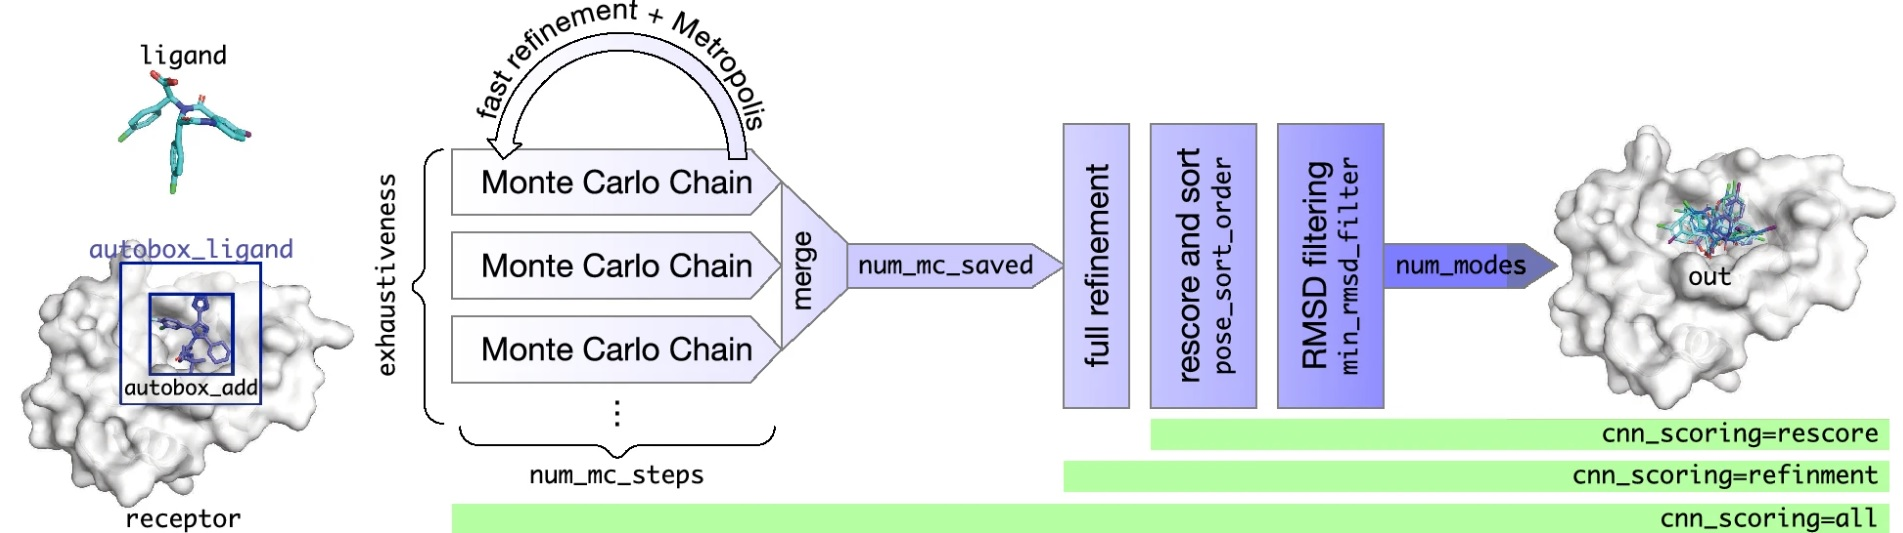
\includegraphics[scale=0.35]{images/gnina_pipeline.jpg}
    \caption[Pipeline di docking seguita da GNINA.]{Pipeline di docking seguita da GNINA. A sinistra, viene mostrata la differenza tra autobox_add ed autobox_ligand. A seguito, vengono mostrate le fasi del processo di docking, fornendo indicazioni sui parametri coinvolti, modificabili dall'utente. Fonte: \cite{mcnutt_gnina_2021}}
    \label{fig:gnina_pipeline}
\end{figure}

Le conformazioni con il punteggio più alto vengono quindi perfezionate applicando nuovamente una funzione di scoring, empirica o CNN, al fine di ottenere la posa localmente ottimale.
Il perfezionamento sposta la posa del ligando a un minimo di energia locale utilizzando i gradienti della funzione di scoring. Dopo che la posa del ligando è stata perfezionata, le affinità finali e i punteggi vengono calcolati per la posa utilizzando i modelli CNN specificati e/o la funzione di punteggio specificata. Infine, le conformazioni del punteggio più alto sono ordinate ed esportate con Open Babel \cite{mcnutt_gnina_2021}. 

% modello
\subsection{Modelli CNN in GNINA}
Dopo aver introdotto nella Sezione \ref{cnn} la struttura di una rete neurale convoluzionale ed i layers più comuni, è possibile farsi un'idea più chiara del modello utilizzato da GNINA per valutare le pose. 

\begin{figure}[H]
    \centering
    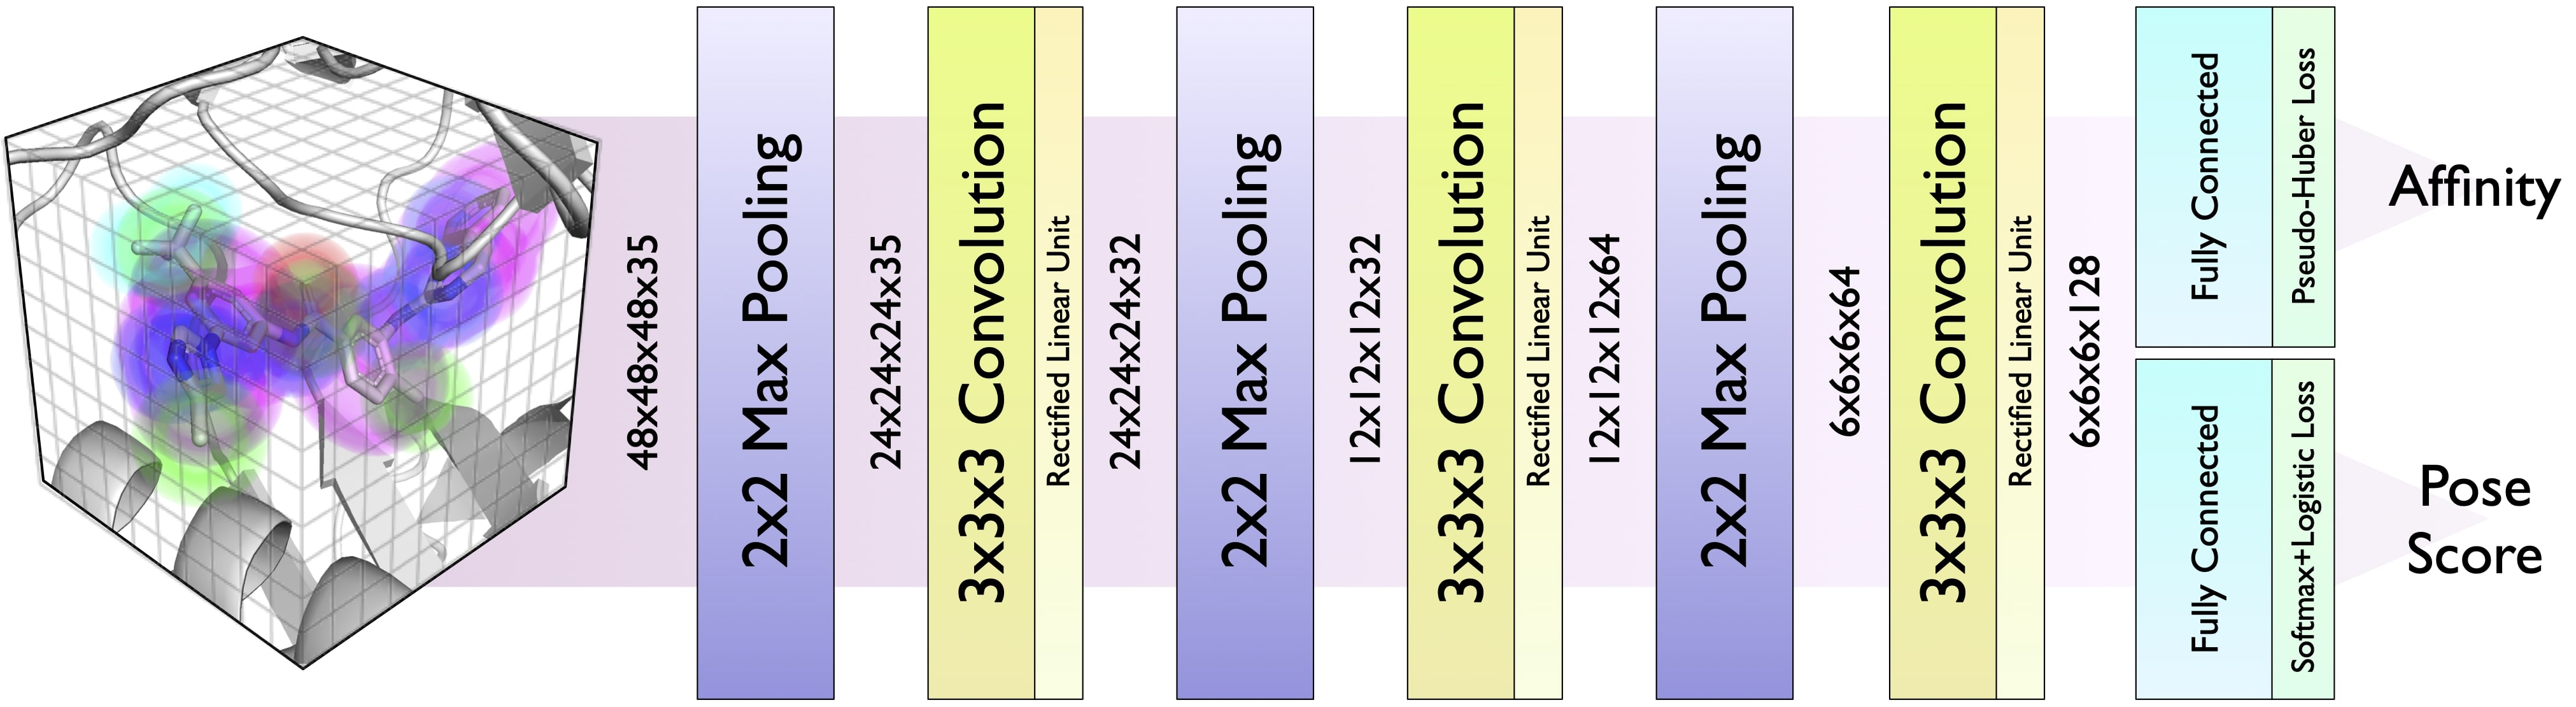
\includegraphics[scale=0.09]{images/cnn_model.jpg}
    \caption[Modello CNN predefinito utilizzato da GNINA.]{Modello CNN predefinito utilizzato da GNINA. In generale le reti convoluzionali sono formate da una sequenza di layer convoluzionali e di pooling, seguita da una rete di classificazione. Fonte: \cite{mcnutt_gnina_2021}}
    \label{fig:cnn_model}
\end{figure}

La funzione di scoring CNN predefinita è un insieme di 5 modelli selezionati per bilanciare le prestazioni di previsione della posa e il tempo di esecuzione: dense, general\_default2018\_3, dense\_3, crossdock\_default2018 e redock\_default2018 \cite{mcnutt_gnina_2021}.


Le funzioni di scoring CNN possono essere specificate fornendo dei file di modello e/o di pesi oppure selezionando un modello built-in. 
I modelli CNN built-in disponibili riguardano crossdock\_ default2018, dense, general\_default2018, redock\_default2018, e default2017, ognuno di questi è addestrato utilizzando un diverso dataset di training e/o un'architettura di modello differente. Inoltre, ogni modello, eccetto per default2017, ha cinque varianti che sono addestrate sugli stessi dati e hanno la stessa architettura, ma sono inizializzati con un seme casuale diverso \cite{mcnutt_gnina_2021}. 


Per ogni tipo di modello CNN, il nome del modello di base si riferisce alla variante con le prestazioni di docking più elevate, e le restanti varianti sono numerate sequenzialmente (ad esempio general\_default2018, general\_ default2018\_1, general\_default2018\_2, general\_default2018\_3, e general\_ default2018\_4); l'insieme di queste cinque varianti è denotato con '\_ensemble' (ad esempio general\_default2018\_ensemble) \cite{mcnutt_gnina_2021}. 

I calcoli ad alte prestazioni della CNN sono eseguiti utilizzando cuDNN, un framework di deep learning  ottimizzato per le GPU, incluso in Caffe. Questi modelli sono addestrati per predire sia la qualità della posa (una probabilità che la posa abbia un RMSD basso rispetto alla posa di legame) e l'affinità di legame (pK). 
Il punteggio della posa è utilizzato per tutti i processi di ottimizzazione della posa \cite{mcnutt_gnina_2021}.

Di seguito sono riportati alcuni dei modelli finalizzati a scopi differenti, come la qualità della posa per HiRes Pose oppure la predizione di affinità migliore come HiRes Affinity.
\begin{figure}[H]
    \centering
    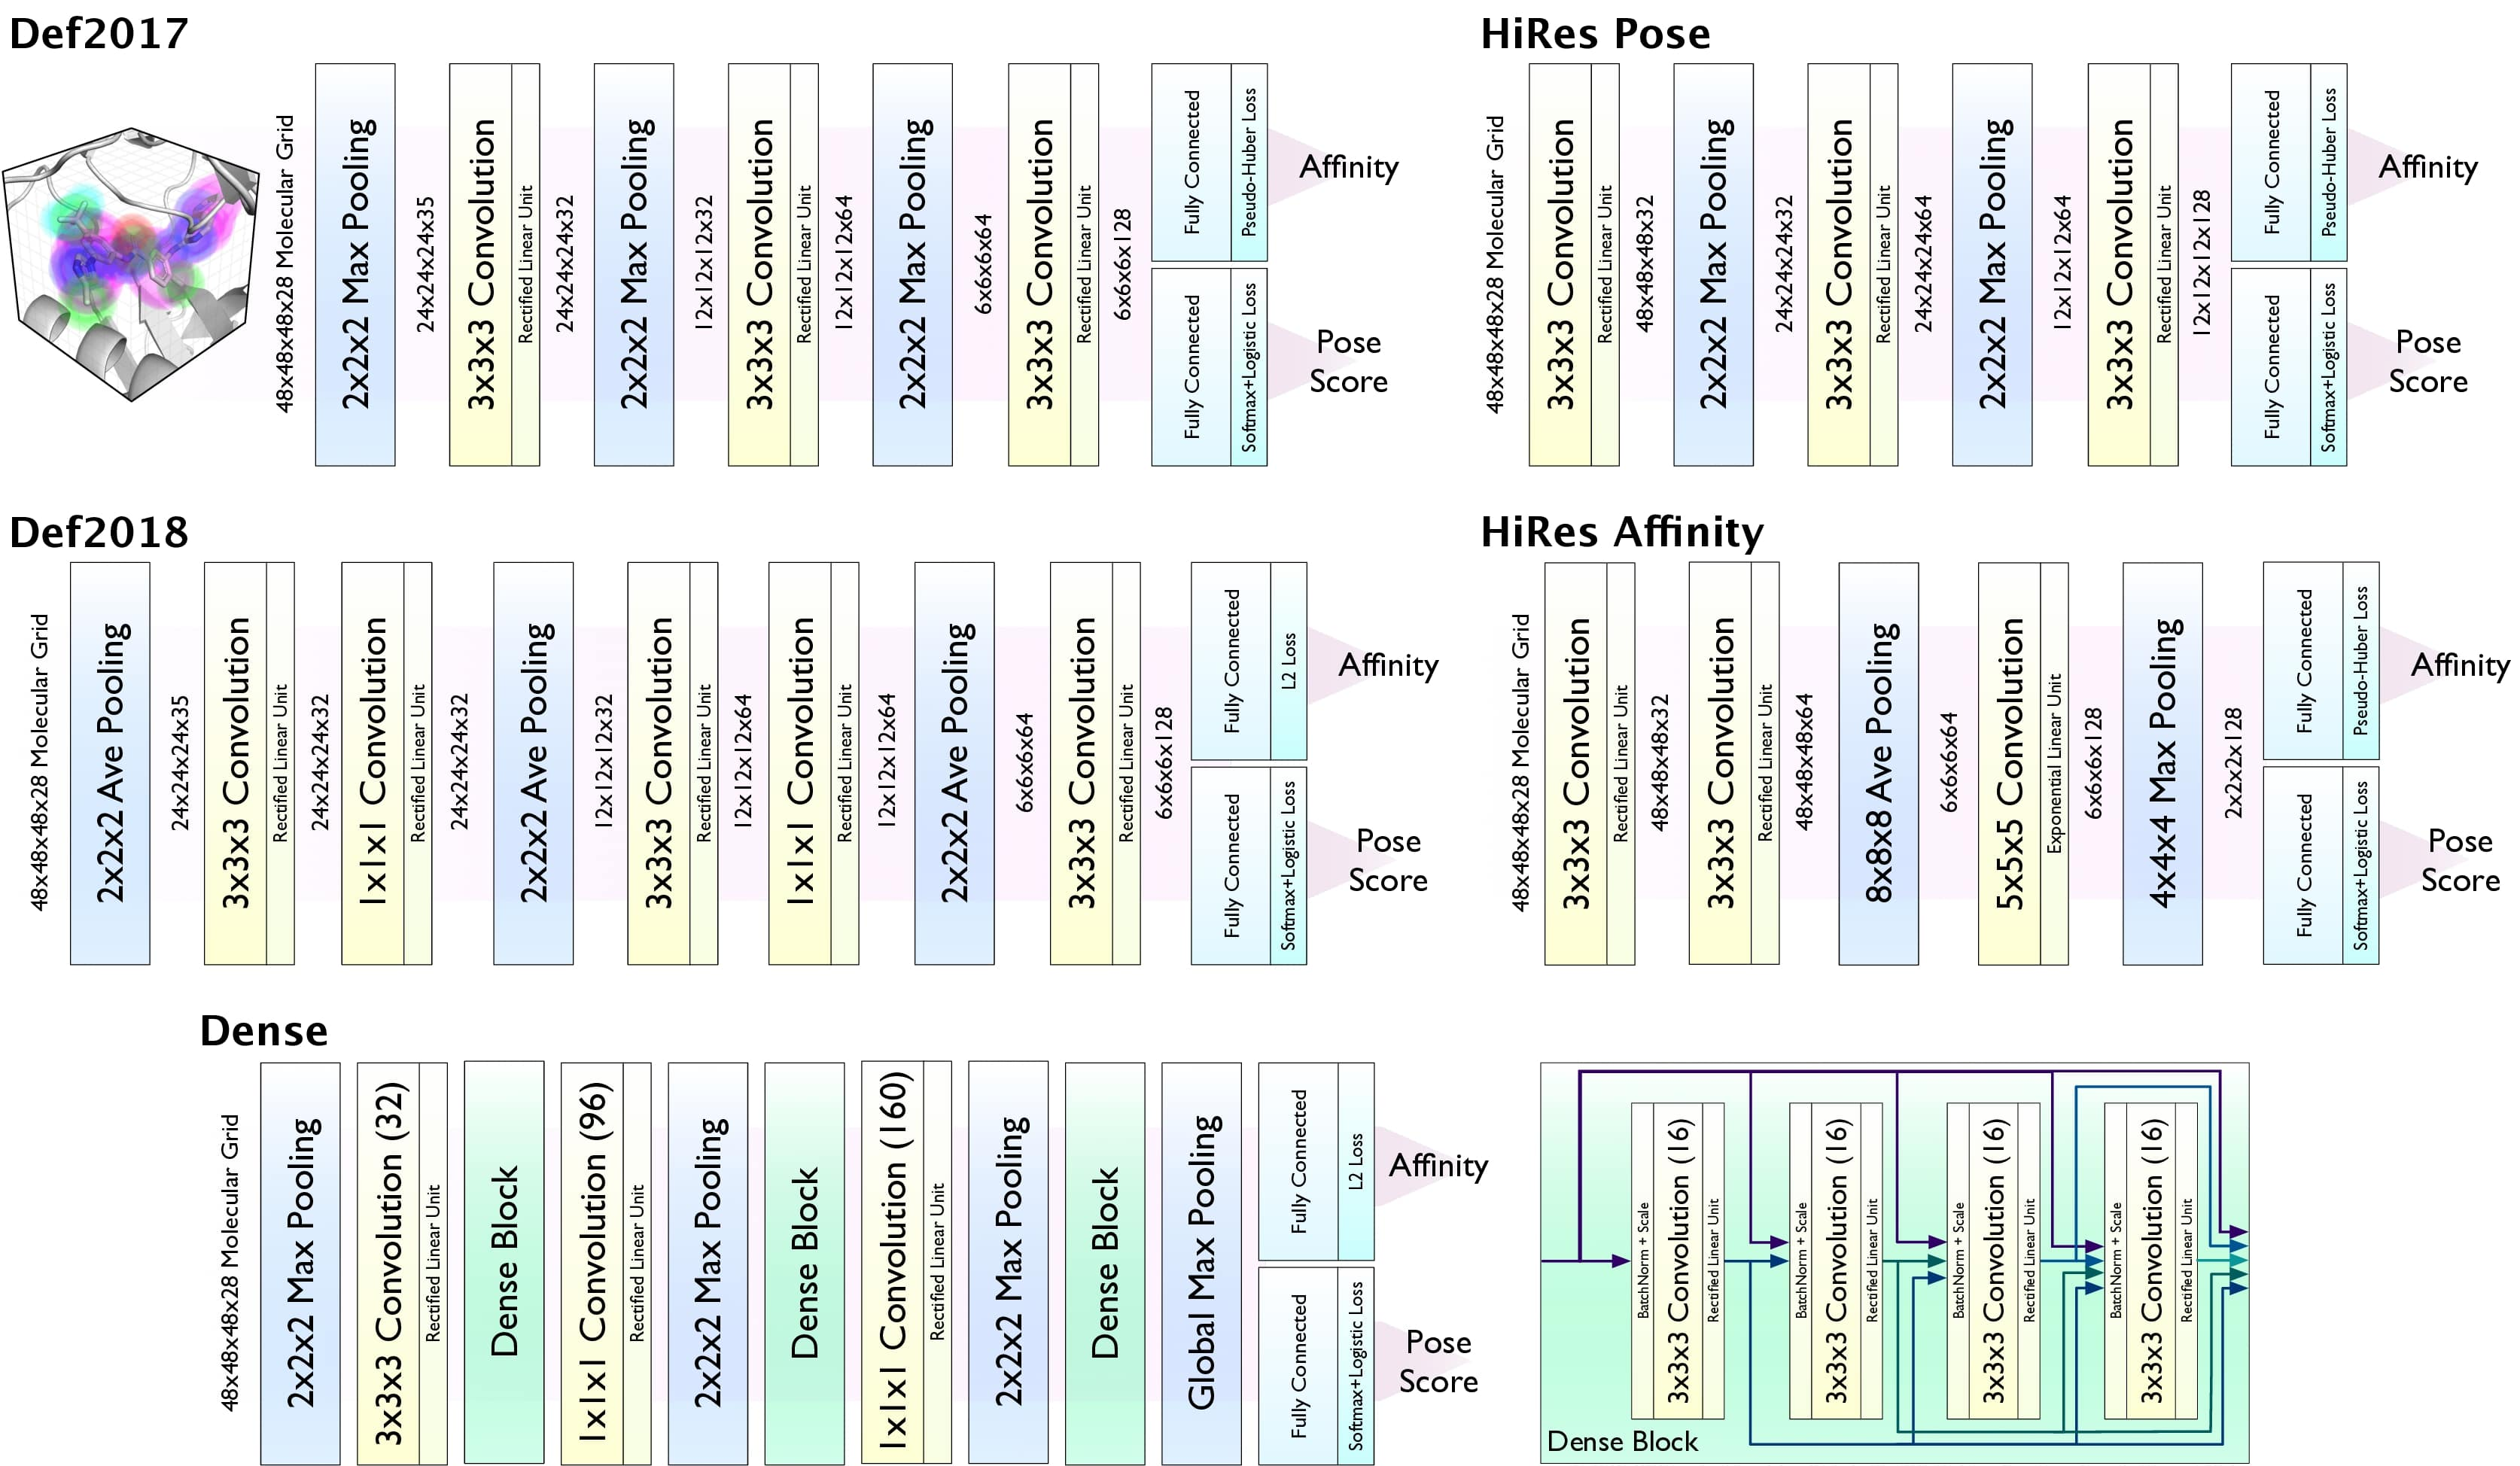
\includegraphics[scale=0.12]{images/models.jpg}
    \caption[Esempi di modelli CNN built-in di GNINA.]{Esempi di modelli CNN built-in di GNINA. I modelli sono etichettati con i loro nome ed per ciascun modello è riportata la propria struttura. Fonte: \cite{mcnutt_gnina_2021}}
    \label{fig:models}
\end{figure}

\subsection{Parametri della CNN in GNINA} \label{cnn_params}
I parametri messi a disposizione per l'utilizzo della CNN nel docking molecolare sono molteplici. Tuttavia, ci focalizziamo sui parametri interessanti ed utilizzati per l'analisi sperimentale proposta dall'elaborato.

Un modello CNN prevede sia la qualità della posa (CNNScore) che l'affinità di legame (CNNaffinity) per ciascuna delle conformazioni prodotte da GNINA. 

Il parametro \textbf{CNNscore} è una stima della bontà della posa ed è un valore compreso tra 0 e 1 che viene utilizzato per classificare le pose del ligando. Un valore di CNNscore pari ad 1 denota una posa del ligando perfetta (rispetto al ligando naturale ove presente). Tendenzialmente, le pose di ligandi molto vicine al recettore, ovvero entro un valore di RMSD inferiore a 2, risultano essere qualitativamente migliori secondo questo criterio \cite{mcnutt_gnina_2021}.

Il parametro \textbf{CNNaffinity} è l'affinità prevista dopo aver stabilito una posa valida nel processo di docking, in questo caso come determinato dalla CNN. E' misurata in unità \(pK\)\footnote{Il valore \(pK\) è un metodo utilizzato per indicare la forza di un composto, relativamente alla costante di dissociazione \(K\).
Un valore di \(pK\) basso indica un composto forte.} \cite{mcnutt_gnina_2021}.
%CNNvariance è la varianza delle affinità previste nell'insieme. Non corrisponde ad un punteggio, ma una misura dell'incertezza. 
%CNN\_VS è la combinazione tra il valore di CNNaffinity ed la bontà della posa CNNscore ed è ottenuta considerando la CNNaffinity della posa migliore ovvero quella con il CNNscore più alto oppure effettuando il prodotto tra CNNaffinity e CNNscore. E' una metrica di valutazione per analisi di virtual screening.

Il parametro \textbf{autobox\_ligand} è ereditato da \textit{smina} e consente di creare una box che inscrive esattamente le coordinate dell'atomo del ligando fornito ed in seguito espansa con il parametro autobox\_add (predefinito 4Å) in ogni dimensione \cite{mcnutt_gnina_2021}.

Il parametro \textit{cnn\_scoring} determina in quali punti della procedura di docking viene utilizzata la funzione di scoring CNN:
\begin{itemize}
    \item \textbf{none} (nessuno) - nessuna CNN utilizzata per il docking. Utilizza la funzione di scoring Vina durante l'intero processo;
    \item \textbf{rescore (predefinito)} - la CNN è utilizzata per riclassificare le pose finali. Risulta essere l'opzione meno costosa dal punto di vista computazionale, tra quelle che coinvolgono la CNN;
    \item \textbf{refinement} (perfezionamento) - la CNN è utilizzata per perfezionare le pose dopo le catene Monte Carlo e per il ranking finale delle pose di output. Risulta essere 10 volte più lento dell'opzione \textit{rescore} quando si utilizza una GPU;
    \item \textbf{all} (tutto) - la CNN è utilizzata come funzione di scoring durante l'intero processo. Questo risulta essere estremamente intensivo dal punto di vista computazionale e non consigliato \cite{mcnutt_gnina_2021}.
\end{itemize}
Le opzioni elencate ed illustrate nella Figura \ref{fig:cnn_scoring} per il parametro \textit{cnn\_scoring} verranno esplicate dettagliatamente nella Sezione \ref{cnn_scoring_method}.

Le pose risultanti vengono rivalutate e ordinate attraverso la selezione del parametro \textbf{pose\_sort\_order}:
\begin{itemize}
    \item \textbf{CNNscore (predefinito)} - le pose con la più alta probabilità di avere un RMSD basso secondo la CNN sono classificate più alte;
    \item \textbf{CNNaffinity} - le pose con la più alta affinità di legame prevista dalla CNN sono classificate più alte;
    \item \textbf{Energy} - le pose con l'energia più bassa o affinità predetta dalla funzione di scoring Vina sono classificate più alte;
\end{itemize}

Si nota che la modifica del criterio di ordinamento può modificare le pose restituite, non solo il loro ordinamento.

% CNN scoring method
\subsection{Funzione di scoring CNN} \label{cnn_scoring_method}
GNINA consente l'utilizzo della CNN in varie fasi del processo di docking molecolare. 
Se la CNN non viene utilizzata affatto nel calcolo del punteggio (opzione \textit{"none"}), la pipeline di docking molecolare è essenzialmente la stessa di \textit{smina}. 
L'opzione \textit{rescore} ha il costo computazionale più basso delle opzioni che utilizzano i modelli CNN.
Con questa opzione i modelli CNN vengono utilizzati per valutare e riordinare le conformazioni del ligando selezionate e perfezionate dalla funzione di scoring non-CNN, la funzione di scoring predefinita Vina \cite{mcnutt_gnina_2021}. 

Per un costo computazionale aggiuntivo, è possibile specificare l'opzione "refinement" per utilizzare i modelli CNN per il perfezionamento dei ligandi dopo che sono stati selezionati dalle catene Monte Carlo. 
Oltre a perfezionare le conformazioni del ligando, i modelli CNN vengono utilizzati per valutare e riordinare le pose di output, come fa l'opzione "rescore". Tuttavia, le catene Monte Carlo continuano a utilizzare la funzione di scoring non-CNN \cite{mcnutt_gnina_2021}. 

\begin{figure}[H]
    \centering
    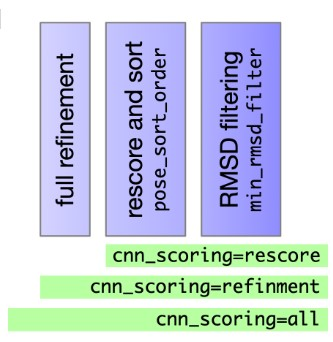
\includegraphics{images/cnn_scoring.jpg}
    \caption[Fasi ricoperte dalle opzioni per il parametro cnn\_scoring.]{Illustrazione grafica delle fasi ricoperte per ciascun opzione del parametro cnn\_scoring. L'opzione \textit{all} applica il modello CNN all'intera pipeline; l'opzione \textit{refinement} è applicata alle fasi mostrate; l'opzione \textit{rescore} applica il modello CNN solo alle ultime due fasi prima di fornire l'output. Fonte: \cite{mcnutt_gnina_2021}}
    \label{fig:cnn_scoring}
\end{figure}

Il processo di \textit{refinement} o perfezionamento con i modelli CNN non è raccomandato in quanto il costo di calcolo è significativo e le prestazioni sono inferiori rispetto al semplice utilizzo dei modelli CNN per rivalutare le pose perfezionate dalla funzione di scoring Vina \cite{mcnutt_gnina_2021}.

L'opzione \textit{all} utilizza i modelli CNN come funzione di scoring nel corso della procedura di docking molecolare ed ha il costo computazionale più alto per ordini di grandezza. Il modello CNN viene utilizzato per il processo di selezione all'interno delle catene Monte Carlo, il processo di \textit{refinement} dopo la selezione Monte Carlo e nel calcolo del punteggio e del riordinamento delle pose prima dell'output. 
Questa opzione è molto impegnativa dal punto di vista computazionale poiché la CNN viene regolarmente interrogata per l'energia di una particolare conformazione durante la procedura di campionamento Monte Carlo \cite{mcnutt_gnina_2021}. 

GNINA consente di combinare le funzioni di scoring CNN e non-CNN, attraverso l'utilizzo di alcuni parametri, sia nella fase di perfezionamento che nel calcolo del punteggio di una certa posa.
L'utilizzo classico delle CNN all'interno della pipeline di docking di GNINA richiede un'elevata precisione limitando, al tempo stesso, i costi computazionali \cite{mcnutt_gnina_2021}.


% input\output
\subsection{Formato dei dati di input e di output in GNINA}
Le strutture del recettore e del ligando possono essere fornite in qualsiasi formato, grazie alla facile gestione attraverso OpenBabel. Questa è una delle funzionalità ereditate da \textit{smina}. 

I parametri di output come CNNscore, CNNaffinity, così come la struttura stessa della posa finale, sono memorizzati nel file di output. Tendenzialmente, se si è interessati ai parametri allora il formato di output preferito dovrebbe essere il formato SDF.


\section{AutoDock Vina} 
Il software AutoDock Vina, progettato e realizzato dal Dr. Oleg Trott presso lo Scripps Research Institute e pubblicato nel 2009 sotto licenza Apache open source, è stato sviluppato per soddisfare l'esigenza di un metodo di docking che non richieda una conoscenza approfondita da parte degli utenti. È altamente ottimizzato per eseguire esperimenti di docking utilizzando metodi predefiniti ben testati  \cite{forli_computational_2016, eberhardt_autodock_nodate}. 

E' stato progettato per essere uno strumento di docking computazionale generico, che accetta file di coordinate per recettore e ligando ed effettua predizioni sulle conformazioni proteina-ligando ottimali \cite{forli_computational_2016}.
AutoDock Vina rappresenta un punto di riferimento per il docking computazionale e per tutte le sue applicazioni.

\subsection{Funzione di scoring Vina} \label{scoring_function_vina}
In Autodock Vina, per determinare quale ligando ha un'interazione complessa stabile con la proteina, la posa viene valutata in termini di "binding energy" o più comunemente affinità.
La funzione di scoring Vina è stata progettata per risultare un ottimo compromesso tra previsione della posa e dell'affinità e tempo di esecuzione ed è una somma pesata di interazioni atomiche \cite{koes_lessons_2013}. 

Ciascuno di questi termini rappresenta generalmente un importante fattore energetico nel legame proteina-ligando. 
Ci sono diversi parametri coinvolti in ciascuna di queste funzioni che possono essere modificati per migliorare le previsioni. Infine, ogni termine viene pesato (moltiplicato per una costante) prima di essere aggiunto all'affinità di legame finale prevista \cite{quiroga_vinardo_2016}. 

L'energia di legame è prevista come la somma delle interazioni di coppie di atomi dipendenti dalla distanza \ref{eq:1}.

\begin{equation} \label{eq:1}
    E = \sum{e_{pair}}{(d)}
\end{equation} 

Qui \(d\) è la distanza superficiale calcolata con l'Equazione \ref{eq:2}, dove r è la distanza interatomica e \(R_i\) e \(R_j\) sono i raggi degli atomi nella coppia \cite{quiroga_vinardo_2016}. 

\begin{equation} \label{eq:2}
    d = r - R_i - R_j
\end{equation} 

Ogni coppia di atomi interagisce attraverso un'interazione sterica data dai primi tre termini dell'Equazione \ref{eq:3}. 
Inoltre, a seconda del tipo di atomo, potrebbero esserci interazioni idrofobiche e non direzionali di legame a idrogeno, date dagli ultimi due termini dell'Eq \ref{eq:3} \cite{quiroga_vinardo_2016}.

\begin{equation} \label{eq:3}
    e_{pair}(d) = 
    \begin{cases}
        w_1 * \text{Gauss}_1(d) +\\
        w_2 * \text{Gauss}_2(d) +\\
        w_3 * \text{Repulsion}(d) +\\
        w_4 * \text{Hydrophobic}(d) +\\
        w_5 * \text{HBond}(d)
    \end{cases}
\end{equation} 

I pesi dei termini sono stati calcolati tramite un adattamento non lineare ai dati strutturali. La Tabella \ref{vina_weights} riporta i termini ed i pesi riferiti nell'Equazione \ref{eq:3} \cite{quiroga_vinardo_2016}.

\begin{table}[H] 
\centering
\begin{tabular}{|l|c|}
\hline
\rowcolor[HTML]{C0C0C0} 
\multicolumn{1}{|c|}{\cellcolor[HTML]{C0C0C0}\textbf{Termine}} & \textbf{Peso} \\ \hline
Gauss\_1                                                       & -0-0356       \\ \hline
Gauss\_2                                                       & -0.00516      \\ \hline
Repulsion                                                      & 0.840         \\ \hline
Hydrophobic                                                    & -0-0351       \\ \hline
Hydrogen bonding                                               & -0.587        \\ \hline
\end{tabular}
\caption[Termini e pesi della funzione di scoring Vina.]{Termini e pesi della funzione di scoring Vina. I termini sono direttamente codificati nel codice sorgente di AutoDock Vina. Fonte: \cite{trott_autodock_2009}}
\label{vina_weights}
\end{table}

È stato dimostrato che si comporta bene con ligandi con dimensioni e composizione biologiche tipiche in esperimenti di \textit{blind docking}.
Per una descrizione più dettagliata della funzione di scoring Vina, si rimanda il lettore all'articolo originale di Trott e Olson \cite{trott_autodock_2009, quiroga_vinardo_2016}.

Nell'implementazione della funzione di scoring Vina, viene utilizzato il metodo di ottimizzazione non lineare non vincolata \textbf{Broyden-Fletcher-Goldfarb-Shanno}, già descritto nella Sezione \ref{bfgs}.
% input/output
\subsection{Formato dei dati di input ed ouput in AutoDock Vina}
Il successo del docking computazionale e dello screening virtuale richiede un'attenta attenzione alla qualità delle coordinate utilizzate per recettori e ligandi. AutoDock Vina utilizza una rappresentazione semplificata delle molecole, memorizzata nel formato PDBQT, un'estensione del formato PDB \cite{forli_computational_2016}.

Ciò semplifica l'utilizzo di Vina con il software ausiliario esistente sviluppato per AutoDock, come AutoDock Tools, per la preparazione dei file, la scelta dello spazio di ricerca e la visualizzazione dei risultati. \cite{trott_autodock_2009}

Il formato PDBQT è un formato più ricco di espressività rispetto al formato standard PDB in quanto, permette di modellare la struttura molecolare come una struttura ad albero.

\begin{figure}[H]
    \centering
    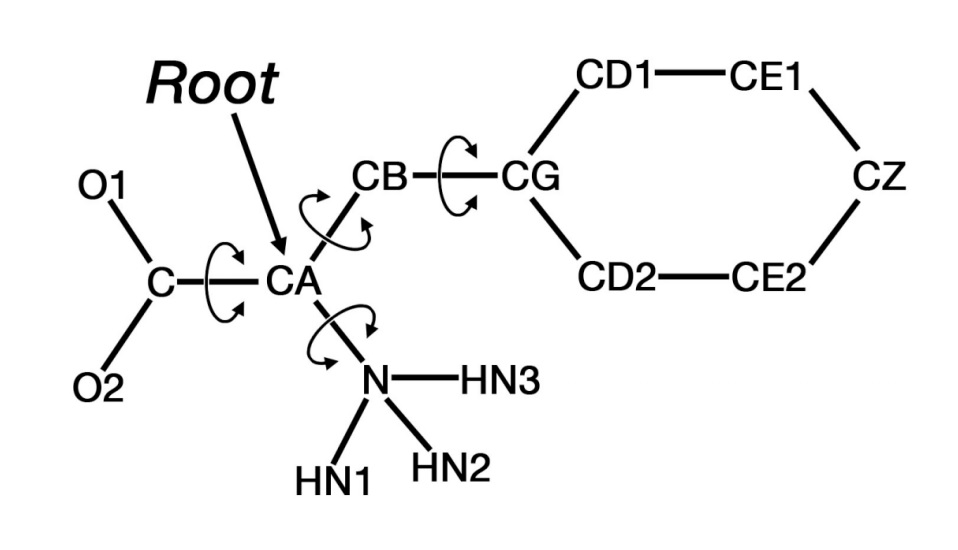
\includegraphics[scale=0.5]{images/pdbqt.jpg}
    \caption[Rappresentazione grafica del formato PDQBT.]{Rappresentazione grafica della struttura ad albero codificata all'interno del formato PDQBT. Fonte: \cite{eberhardt_autodock_nodate}}
    \label{fig:pdbqt}
\end{figure}

\section{Linguaggi di programmazione}
\subsection{Python}
% Linguaggio di programmazione utilizzato: Python, motivare l'utilizzo (script)
L'applicazione è scritta prevalentemente in \textbf{Python3}, anche se alcuni script fanno riferimento a Python2. La scelta di tale linguaggio è stata pressochè obbligata dalla necessità di interagire con framework e librerie diversi, al fine di sviluppare le funzionalità dell'applicazione realizzata.
La potenza di questo linguaggio, dalla facilità di gestione delle strutture dati alla capacità di essere \textit{platform-independent}, insieme alla vastità di librerie presenti per gli scopi più disparati, sono stati fondamentali per lo sviluppo dell'applicazione.

\subsubsection{Librerie utilizzate}
In questa Sezione, vengono semplicemente elencate le principali librerie utilizzate nell'applicazione proposta. Una trattazione più dettagliata è fornita nell'elaborato del collega Alfredo Mungari.

Librerie come \textit{Pandas} e \textit{NumPy} sono ampiamente utilizzate nell'ambito della Data Science, ormai integrate di default in ambienti di calcolo scientifico come Anaconda.

Per la selezione delle strutture, sono state utilizzate \textit{rcsbsearch}, \textit{ProDy} e \textit{PubChemPy}.
Per la trattazione delle strutture e dei file relativi, sono state utilizzate \textit{biopandas}, \textit{biopython}, \textit{OpenBabel} e \textit{ProDy}.
Per l'estrazione delle interazioni e la realizzazione dei grafici sono state utilizzate rispettivamente \textit{MolKit} e \textit{Matplotlib}.

Per il calcolo della Minimized Symmetric-Corrected RMSD, è stata utilizzata la libreria \textbf{spyrmsd}, la quale fornisce solidi calcoli della RMSD con correzione della simmetria attraverso un'API semplice e pulita che è facile da integrare nelle librerie e pipeline Python esistenti \cite{meli_spyrmsd_2020}.


\subsection{Shell scripting}
L'ambiente UNIX/Linux è stata una scelta obbligata anche in questo caso. La motivazione è data da diversi fattori: in primis, le applicazioni di docking computazionale sono sviluppate ed utilizzate principalmente in ambiente Linux; per questo motivo, la conoscenza del dominio applicativo è stata rilevante nella scelta. 

In secundis, la scelta è stata dettata dal fatto che alcuni componenti fondamentali, come i collegamenti in Python di OpenBabel, fossero disponibili ed utilizzabili effettivamente solo su alcune versioni di Linux. A tal proposito, il sistema operativo utilizzato 
durante lo sviluppo dell'applicazione è stato Ubuntu Fossa 20.04.

Per questa ragione, lo shell scripting è stato introdotto in questa sezione. Diverse procedure sono state automatizzate attraverso il \textbf{Bash scripting} come la procedura di docking sia nel caso di AutoDock Vina che di GNINA.


\section{Piattaforme software}
Le piattaforme software utilizzate costituiscono praticamente l'insieme di strumenti standard nella trattazione di strutture molecolari

\subsection{OpenBabel}
% OpenBabel (brevemente)
\textbf{OpenBabel} è un toolbox chimico che consente la lettura e la scrittura di oltre 100 formati di file chimici, viene utilizzato per analizzare gli input, consentendo formati di dati strutturali comunemente usati (ad es. PDB, sdf, mol, ecc.) così come versioni gzip di tali file da utilizzare.


\subsection{MGLTools} 
La suite software \textbf{MGLTools} è stata sviluppata nel laboratorio Sanner presso il Center for Computational Structural Biology (CCRB) precedentemente noto come Molecular Graphics Laboratory (MGL) dello Scripps Research Institute per la visualizzazione e l'analisi delle strutture molecolari. MGLTools comprende:
\begin{itemize}
    \item \textbf{Python Molecular Viewer (PMV)}, un visualizzatore molecolare di uso generale;
    \item \textbf{AutoDockTools (ADT)},una serie di comandi PMV sviluppati specificamente per supportare gli utenti di AutoDock;
    \item \textbf{Vision}, un ambiente di programmazione visiva.
\end{itemize}

Questi strumenti software sono altamente integrati e basati su componenti software riutilizzabili implementati in Python e C++ (con collegamenti Python).

%% spiegare utilizzo di script come prepare_receptor e prepare_ligand.
Inoltre, un contributo significativo da parte di questa suite deriva dai comandi forniti per la preparazione di recettori e ligandi come \textbf{prepare\_receptor} e \textbf{prepare\_ligand}, ampiamente utilizzati nelle operazioni classiche di preparazione delle strutture, risultando quasi uno standard \textit{de facto}.

\subsection{AutoDockTools} \label{autodocktools}
% Suite AutoDock 
AutoDock è una suite gratuita di software open-source  per il docking computazionale e lo screening virtuale di piccole molecole ai recettori macromolecolari. La suite comprende attualmente diversi strumenti complementari tra cui AutoDock Vina ed AutoDockTools \cite{forli_computational_2016}.

\textbf{AutoDockTools} è uno strumento grafico interattivo per la preparazione delle macromolecole, il docking, l'analisi spaziale degli atomi e delle interazioni all'interno delle strutture \cite{forli_computational_2016}.


\begin{table}[H]
\centering
\resizebox{\columnwidth}{!}{%
\begin{tabular}{|l|l|}
\hline
\rowcolor[HTML]{C0C0C0} 
\multicolumn{1}{|c|}{\cellcolor[HTML]{C0C0C0}\textbf{Metodo}}                                        & \multicolumn{1}{c|}{\cellcolor[HTML]{C0C0C0}\textbf{Descrizione}}                                                                                                                  \\ \hline
\textit{\begin{tabular}[c]{@{}l@{}}Singolo esperimento di docking con \\ AutoDock Vina\end{tabular}} & \begin{tabular}[c]{@{}l@{}}Metodo di docking di base per lo studio di un singolo\\ ligando con un singolo recettore\end{tabular}                                                   \\ \hline
\textit{\begin{tabular}[c]{@{}l@{}}Singolo esperimento di docking con\\ AutoDock\end{tabular}}       & \begin{tabular}[c]{@{}l@{}}Metodo di docking di base per lo studio di un singolo \\ ligando con un singolo recettore, con esplicito calcolo\\ delle mappe di affinità\end{tabular} \\ \hline
\textit{\begin{tabular}[c]{@{}l@{}}Virtual Screening con Raccoon2 e \\ AutoDock Vina\end{tabular}}   & \begin{tabular}[c]{@{}l@{}}Screening virtuale di una libreria di ligandi con un \\ singolo recettore, spesso utilizzato per la scoperta\\ di farmaci\end{tabular}                  \\ \hline
\textit{\begin{tabular}[c]{@{}l@{}}AutoDock Vina con catene laterali\\ flessibili\end{tabular}}      & \begin{tabular}[c]{@{}l@{}}Metodo di docking per un singolo ligando con un \\ singolo recettore, includendo una flessibilità limitata\\ del recettore\end{tabular}                 \\ \hline
\textit{\begin{tabular}[c]{@{}l@{}}Predizione di sito attivo con\\ AutoLigand\end{tabular}}          & \begin{tabular}[c]{@{}l@{}}Metodo di analisi dei siti di legame del recettore, per\\ la predizione di siti attivi\end{tabular}                                                     \\ \hline
\textit{\begin{tabular}[c]{@{}l@{}}Docking con molecole d'acqua \\ esplicite\end{tabular}}           & \begin{tabular}[c]{@{}l@{}}Metodo di docking avanzato per un singolo ligando \\ con un singolo recettore includendo molecole\\ d'acqua esplicite che formano ponti\end{tabular}    \\ \hline
\end{tabular}%
}
\caption[Esempi di applicazione della suite AutoDock.]{Esempi di applicazione della suite AutoDock. Fonte: \cite{forli_computational_2016}}
\end{table}

La suite AutoDock, incluso il codice sorgente, è disponibile gratuitamente ed è stata ampiamente utilizzata nella ricerca e nella scoperta di farmaci \cite{forli_computational_2016}.



\section{Piattaforme hardware}
Come sarà più chiaro ed argomentato nei capitoli successivi, il processo di docking è abbastanza intenso in termini di carico computazionale nel nostro caso ed in termini di potenza di calcolo necessaria. Per soddisfare tale esigenza si è ricorso al \textbf{cloud computing}\footnote{Il cloud computing indica, in informatica, un paradigma di erogazione di servizi offerti su richiesta da un fornitore a un cliente finale attraverso la rete internet, a partire da un insieme di risorse preesistenti, configurabili e disponibili in remoto sotto forma di architettura distribuita. } attraverso l'utilizzo di piattaforme hardware importanti.

\subsection{PurpleJeans}
Il cluster di calcolo purpleJeans è una risorsa condivisa utilizzata da tutta la comunità RCF (Research Computing Facilities), che utilizza uno scheduler per gestire le richieste di accesso alle risorse di calcolo, dette job. In particolare, viene utilizzato il gestore delle risorse di Slurm per pianificare i lavori, nonché l’accesso interattivo ai nodi di calcolo.
Slurm è un sistema open source, tollerante ai guasti e altamente scalabile per la gestione dei cluster e la pianificazione (sheduling) dei job per cluster Linux grandi e piccoli.

L'accesso a questo cluster di calcolo è stato fornito dall'Università degli Studi di Napoli 'Parthenope' ed in particolare grazie al Prof. Raffaele Montella, oltre al mio relatore Prof. Angelo Ciaramella.

Il cluster di calcolo \textbf{purpleJeans} è costituito da nodi di calcolo con diverse architetture e configurazioni. Una partizione è una raccolta di nodi di calcolo che hanno tutti la stessa o simile architettura e configurazione. Attualmente, purpleJeans ha le seguenti partizioni:

\begin{figure}[H]
    \centering
    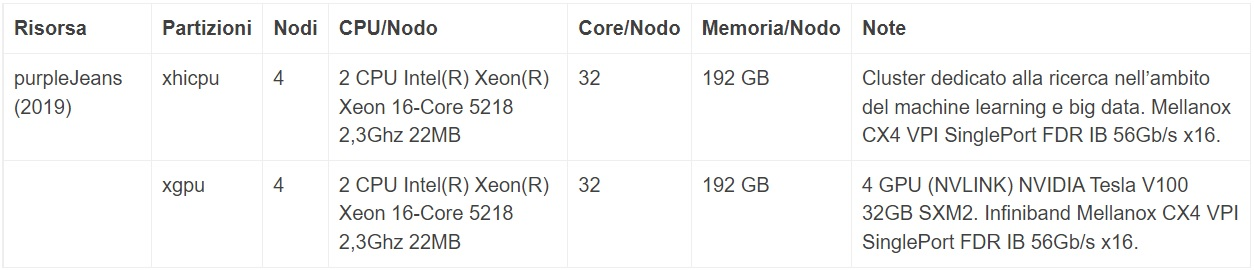
\includegraphics[scale=0.5]{images/purple_jeans.jpg}
    \caption[Scheda tecnica di purpleJeans.]{Scheda tecnica di purpleJeans. \\
    Fonte: \url{https://rcf.uniparthenope.it/it/userguide/}}
    \label{fig:purple_jeans}
\end{figure}


L'utilizzo di purpleJeans è stato fondamentale nell'ottenimento dei risultati del docking proposti per il software AutoDock Vina.

\subsection{Google Colab}
Nonostante esistano diversi servizi di cloud computing, Google Colab è una piattaforma Cloud che permette di eseguire codice direttamente dal browser, sfruttando la potenza di calcolo messa a disposizione da Google ed attraverso i Jupyter Notebook, documenti interattivi in cui è possibile alternare paragrafi testuali a blocchi di codice eseguibili, scritti in Python oppure Shell scripting. 
L'utilizzo di Google Colab ha permesso l'ottenimento dei risultati relativi al docking con GNINA, sfruttando il tipo di runtime GPU, in maniera gratuita seppur con qualche limitazione sulla durata di utilizzo del servizio. 

\chapter{Applicazione realizzata}

\textit{In questo capitolo viene introdotta l'applicazione proposta nell'elaborato in termini di architettura e moduli realizzati ed i passi delle procedure di preparazione e valutazione al fine di ottenere i risultati sperimentali e le relative considerazioni, discusse nei prossimi capitoli. }

\section{Architettura dell'applicazione}
L'applicazione presentata per la comparazione tra software di docking computazionale è organizzata a partire dagli script sviluppati durante il tirocinio interno di circa 300 ore, svolto presso il Consiglio Nazionale delle Ricerche (CNR), alla sede di Napoli.
Sulla base delle analisi proposta per la valutazione dei rischi delle \textit{Apis mellifera} relativamente all'utilizzo dei pesticidi, condotta dal Dott. Ferdinando Febbraio e dalla Dott.ssa Mónica del Águila e seguiti dal Prof. Angelo Ciaramella, è stata realizzata un'applicazione, che fosse in grado di supportare il lavoro di un qualsiasi biologo o biochimico nelle operazioni più classiche di preparazione delle strutture pre-docking, oltre che nell'analisi dei risultati post-docking. Le suddette operazioni, che richiedono un certo livello di \textit{expertize} con i sistemi informativi, sia in termini di manualità sia di ricerca di informazioni, sono spesso procedure meccaniche e macchinose, che rallentano il processo di analisi. Lo sviluppo di tale applicazione ha permesso di automatizzare alcune ma fondamentali operazioni del processo di docking, realizzando un'\textit{Application Program Interface}, più comunemente nota come \textbf{API}, su cui si basa fortemente l'applicazione proposta nell'elaborato. 

L'API è suddivisa in moduli ben distinti che ricoprono le funzionalità dell'applicazione lungo tutta la filiera del docking: dalla fase di preprocessing delle strutture all'analisi delle interazioni dei complessi proteina-ligando. Si è ricorso, quindi, all'utilizzo dei moduli \textbf{MoleculesPreparation} e \textbf{InteractionsAnalysis} per le rispettive fasi di preparazione ed analisi.

I dettagli relativi all'applicazione realizzata durante l'attività di Tirocinio ed ai moduli realizzati saranno definiti esaustivamente nell'elaborato di Tesi triennale in Informatica del collega Alfredo Mungari, prossimo alla laurea nel dicembre 2022, col quale ho condiviso l'intera esperienza di sviluppo.

\section{Scelta del dataset}
A partire dall'esempio di una effettiva applicazione di docking computazionale, presentato precedentemente nella Sezione \ref{Apis mellifera}, la scelta del dataset è ricaduta sulle strutture molecolari tridimensionali della "Apis mellifera" e dei pesticidi coinvolti nella valutazione dei rischi seguita durante il lavoro di tirocinio. Queste strutture indicano rispettivamente l'insieme dei recettori e dei ligandi che saranno utilizzati nel processo di docking, i cui risultati saranno oggetto della comparazione tra i software presentati. 

\subsection{Selezione dei recettori}
Per la selezione dei recettori, si è ricorso al \textbf{Protein Data Bank}, già citato nella Sezione \ref{requirements}. In particolare, la query costruita per recuperare le informazioni dal database considera particolari strutture proteiche che compongono il genoma dell'\textit{Apis mellifera}.

Le api possono essere esposte ai prodotti fitosanitari in due modi: 
\begin{itemize}
    \item per esposizione diretta a \textit{droplets}, che vengono sparse durante l'irrorazione fogliare delle colture, alla polvere della semina durante la semina o all'inalazione di pesticidi volatili durante o dopo l'applicazione alle colture;
    \item dall'esposizione a residui presenti in polline, cera, nettare, miele e gocce di guttazione, che possono derivare dalla contaminazione diretta da spray dei fiori, dalla traslocazione attraverso le piante o dal suolo trattati, o dalla contaminazione diretta durante il trattamento di i favi (solo per le api mellifere);
    \item per esposizione orale ad acqua contaminata \cite{sanchez-bayo_pesticide_2014}.
\end{itemize}

Oltre alle generiche proteine di trasporto, le strutture proteiche selezionate riguardano maggiormente:
\begin{itemize}
    \item le proteine di membrana in quanto alcune di queste sono prese di mira da particolari pesticidi che provocano disturbi alimentari, motori, cognitivi ed infine la morte;
    \item il sistema immunitario per testare le proteine che svolgono un ruolo chiave nell'innescare le risposte immunitarie ai batteri negli insetti;
    \item il sistema olfattivo, anche dette \textit{odorant-binding protein} (OBP), che includono le \textit{pheromone binding protein} (PBP), in quanto sono coinvolte nella rilevazione di odori e feromoni, scaturendo in una segnalazione per attivare un risposta.
\end{itemize}

\begin{figure}
    \centering
    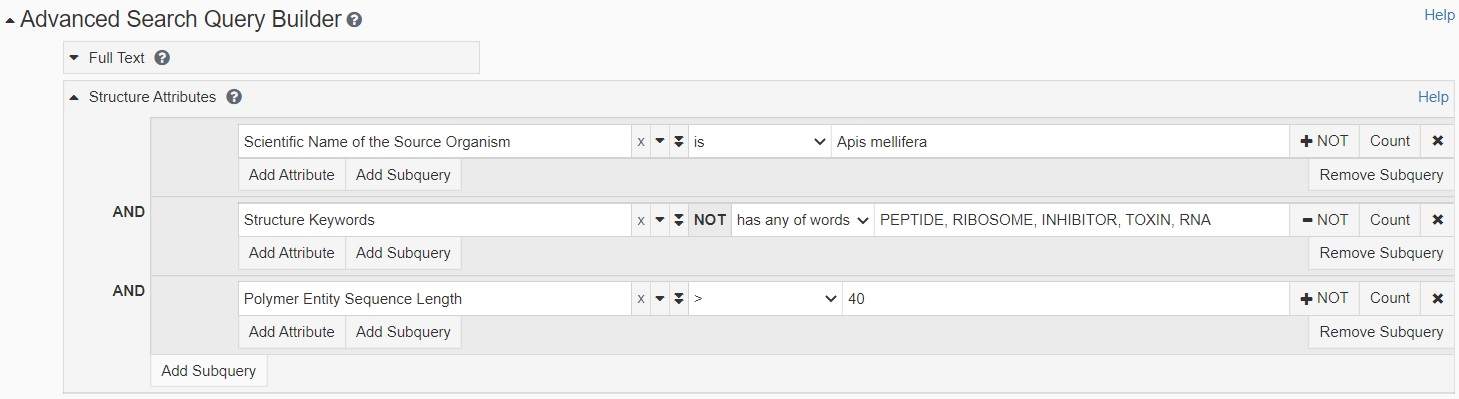
\includegraphics[scale=0.45]{images/chapter3/rcsb_query.jpg}
    \caption[Query per la selezione dei recettori.]{Query per la selezione dei recettori dal sito\\ \url{https://rcsb.org/search/advanced}. La scelta della query e la relativa struttura sono illustrate di seguito, nel testo.}
    \label{fig:rcsb_query}
\end{figure}

La selezione delle proteine appena menzionate avviene, quindi, tramite un'interrogazione del Protein Data Bank su attributi come \textit{Scientific Name of the Organism}, \textit{Polymer Entity Sequence Length} per evitare strutture troppo grandi e le \textit{Structure Keywords} che caratterizzano la struttura.

\subsection{Selezione dei ligandi}
Le molecole dei pesticidi sono state selezionate in base all'elenco delle sostanze attive approvate dal database dei pesticidi dell'Unione Europea. Successivamente, le strutture 3D sono state scaricate da \textbf{PubChem} e dall'\textbf{EU Pesticides Database}. 
I pesticidi le cui strutture erano indisponibili in entrambi i database sono stati esclusi dal dataset finale dei ligandi.

La selezione dei ligandi riguarda le strutture dei pesticidi di vario genere come erbicidi, fungicidi e neonicotinoidi, in particolare i piretroidi, a causa della loro nota tossicità.  


\section{Formato dei dati di input ed output}
Le grid-box sono memorizzate nel formato \textit{.txt} mentre le strutture dei recettori e dei ligandi sono fornite rispettivamente nel formato \textit{.pdb} e \textit{.sdf}.
Sia nel caso di recettori sia nel caso di ligandi, al termine della fase di preparazione ed analogamente nella fase di docking, l'output delle strutture è fornito nel formato \textit{.pdbqt}.

\section{Procedura di preparazione al docking} \label{preparation}
Il protocollo di preparazione al docking utilizzato segue dei passi ben definiti per fornire una base equivalente a partire dalla quale effettuare le valutazioni successive alla fase di docking. Tendenzialmente, le fasi di pre-processing delle strutture di input e di post-processing dei risultati del docking sono condivise per entrambi i software, così da non introdurre difformità a monte del processo di valutazione delle prestazioni. 

La fase di pre-processing delle strutture, quindi, consiste nella preparazione dei recettori e dei ligandi.

\begin{table}[H]
\centering
\resizebox{\columnwidth}{!}{%
\begin{tabular}{cl}
\toprule
\multicolumn{2}{c}{\textbf{Procedura di preparazione}}                                                                                                                                                                                                                                                                                                    \\ \midrule
\multicolumn{2}{c}{\textbf{Preparazione delle strutture}}                                                                                                                                                                                                                                                                                                 \\ \midrule
\multicolumn{1}{c}{\textbf{Recettori}}                                                                                                                                                                    & \multicolumn{1}{c}{\textbf{Ligandi}}                                                                                 \\ \midrule
\multicolumn{1}{l}{\begin{tabular}[c]{@{}l@{}}• separazione dei residui ripetuti\\ • epurazione da catene di eteroatomi\\ • rimozione di catene duplicate\\ • applicazione di prepare\_receptor4.py \\ (modificato)\end{tabular}} & \begin{tabular}[c]{@{}l@{}}• conversione da .sdf a .pdb\\ • conversione da .pdb a .pdbqt\\ • applicazione di prepare\_ligand4.py\end{tabular} \\ \midrule
\end{tabular}%
}
\caption[Riepilogo delle procedura di preparazione.]{Riepilogo delle procedura di preparazione. A sinistra la procedura di preparazione dei recettori, a destra la procedura di preparazione dei ligandi. }
\label{preparation_table}
\end{table}

Per i due software, il concetto di \textit{best binding pose} è notevolmente diverso. 
Il software AutoDock Vina considera la migliore posa tra tutte quelle possibili nello spazio conformazionale di ricerca quella che risulta avere l'\textit{affinità} minore. A parità di affinità, viene selezionata la posa la cui RMSD\footnote{In bioinformatica, la Root Mean Square Deviation delle posizioni atomiche è la misura della distanza media tra gli atomi di proteine sovrapposte.} risulta essere minore.

Nel caso del sofware GNINA, il criterio utilizzato è quello predefinito CNNscore, introdotto nella Sezione \ref{cnn_params}. Tuttavia, nulla vieta di fissare un criterio differente in base al tipo di analisi che si vuole effettuare.


\subsection{Preparazione dei recettori}
Nel caso specifico, la preparazione dei recettori richiede alcune operazioni direttamente implementate ed altre solitamente applicate nella fase di preparazione.

Le operazioni direttamente implementate riguardano la separazione di residui ripetuti, l'epurazione da catene di eteroatomi e la rimozione di catene molecolari duplicate.

La \textbf{separazione dei residui ripetuti} riguarda quelle ripetizioni dei residui nelle catene molecolari della struttura del recettore. Quest'informazione è comunemente nota come \textit{"alternative location"} e codificata come \textit{alt\_loc}. La \textbf{pulizia di catene di eteroatomi} consiste nell'epurazione della struttura da catene formate esclusivamente da eteroatomi, non interessanti per il processo di docking. Successivamente viene eseguita la \textbf{rimozione delle catene molecolari duplicate} e considerate solo catene distinte tra le catene molecolari presenti all'interno della struttura.

Inoltre, la preparazione include la rimozione delle molecole d'acqua e di eventuali ligandi non standard residui, l'aggiunta di atomi di idrogeno polari e cariche di Kollman e l'unione delle cariche e la rimozione di atomi di idrogeno non polari e delle coppie molecolari slegate. Infine, sono state create le \textit{grid-box} con una spaziatura di 3Å (angstroms) per scansionare la superficie della proteina.
Per effettuare queste operazioni, è stato applicato uno script modificato di \textbf{prepare\_receptor4.py} prodotto dallo Scripps Research Institute, distribuito nelle suite MGLTools ed AutoDockFR e comunemente utilizzato nelle fasi di pre-processing dei recettori. Tale modifica consiste nella possibilità di aggiungere cariche di Kollman, piuttosto che esclusivamente cariche di Gasteiger, risultando in un'estensione dello script. 


\subsection{Preparazione dei ligandi}
Relativamente alle strutture dei ligandi, non vengono effettuate particolari operazioni se non la conversione di formato e operazioni svolte comunemente nella preparazione classica dei ligandi. 
A tal proposito, è stato utilizzato \textbf{OpenBabel} per la conversione del formato della struttura e successivamente lo script \textbf{prepare\_ligand4.py}, prodotto dallo Scripps Research Institute, distribuito nelle suite MGLTools ed AutoDockFR.
La preparazione include l'unione delle cariche e la rimozione di atomi di idrogeno non polari e delle coppie molecolari slegate.


\subsection{Fase di docking}
Per i due software in competizione, è mostrato il commando lanciato con i relativi parametri. Per ogni parametro è fornita una breve descrizione.

Di seguito è riportato il comando lanciato per effettuare il docking utilizzando AutoDock Vina e la relativa tabella esplicativa dei parametri.


\begin{minted}[breaklines]{bash}
  $ vina --config <text_file> --receptor <receptor_file> --ligand <ligand_file> --out <output_file> --log <text_file>
\end{minted}
%

\begin{table}[H]
\centering
\resizebox{\columnwidth}{!}{%
\begin{tabular}{cl}
\toprule
\multicolumn{1}{l}{\textbf{Parametro}} & \textbf{Descrizione del parametro}                                                                                                                                                                         \\ \midrule
\textit{--config}                                                         & \begin{tabular}[c]{@{}l@{}}Consente di allegare un file di configurazione, il quale contiene\\ le informazioni come l'\textit{exhaustiveness} e i parametri della grid-box,\\ come file di testo (txt)\end{tabular} \\ \midrule
\textit{--receptor}                                                       & Seleziona il recettore per cui effettuare il docking                                                                                                                                                       \\ \midrule
\textit{--ligand}                                                         & Seleziona il ligando per cui effettuare il docking                                                                                                                                                         \\ \midrule
\textit{--out}                                                            & Consente di esportare la pose con il valore di affinità maggiore                                                                                                                                           \\ \midrule
\textit{--log}                                                            & \begin{tabular}[c]{@{}l@{}}Permette di salvare un file di logging contenente le informazioni\\ dall'avvio del comando fino al termine del docking, come file di\\ testo (txt).\end{tabular}                \\ \bottomrule
\end{tabular}%
}
\caption[Tabella dei parametri per il docking con AutoDock Vina.]{Tabella dei parametri del comando per il docking utilizzando AutoDock Vina. A sinistra sono illustrati i paramentri, a destra la relativa descrizione.}
\end{table}

Di seguito è riportata il comando lanciato per effettuare il docking utilizzando GNINA e la relativa tabella esplicativa dei parametri. Per questioni di chiarezza, sono riportati anche i parametri impliciti e predefiniti della commandline.

\begin{minted}[breaklines]{bash}
  $ gnina --receptor <receptor_file> --ligand <ligand_file> --autobox_ligand <receptor_file> --cnn_verbose
\end{minted}

\begin{table}[H]
\centering
\resizebox{\columnwidth}{!}{%
\begin{tabular}{cl}
\toprule
\textbf{Parametro}           & \textbf{Descrizione del parametro}                                                                                                                      \\ \midrule
\textit{--receptor}          & Seleziona il recettore per cui effettuare il docking                                                                                                    \\ \midrule
\textit{--ligand}            & Seleziona il ligando per cui effettuare il docking                                                                                                      \\ \midrule
\textit{--autobox\_ligand}   & \begin{tabular}[c]{@{}l@{}}Permette di indicare la struttura del recettore contenente il ligando\\ naturale, qualora questo fosse presente\end{tabular} \\ \midrule
\textit{--scoring}           & \begin{tabular}[c]{@{}l@{}}Permette di selezionare la funzione di scoring da utilizzare inizialmente \\ (Vina, predefinito)\end{tabular}                                                                            \\ \midrule
\textit{--cnn\_scoring}      & \begin{tabular}[c]{@{}l@{}}Consente di specificare in quale fase del processo di docking utilizzare\\ la funzione di scoring CNN (rescore, predefinito)\end{tabular}           \\ \midrule
\textit{--pose\_sort\_order} & \begin{tabular}[c]{@{}l@{}}Permette di selezionare il criterio secondo il quale effettuare il ranking\\ delle pose (CNNscore, predefinito)\end{tabular}                         \\ \midrule
\textit{--cnn\_verbose}      & \begin{tabular}[c]{@{}l@{}}Maggiori informazioni sono messe a schermo aumentando la \\ verbosità del software\end{tabular}                              \\ \bottomrule
\end{tabular}%
}
\caption[Tabella dei parametri per il docking con GNINA.]{Tabella dei parametri interessanti, impliciti ed espliciti del comando per il docking utilizzando GNINA. A sinistra sono illustrati i paramentri, a destra la relativa descrizione.}
\end{table}

\section{Procedura di valutazione delle prestazioni} \label{evalutation}
La fase di post-processing, introdotta nella Figura \ref{evaluation_table}, consiste nell'utilizzo di metriche per valutare le prestazioni del docking, in primo luogo della rete neurale convoluzionale applicata nel software GNINA, e successivamente del software AutoDock Vina, che analizzano diversi aspetti del risultato di un esperimento di \textbf{single blind docking}: dalla visualizzazione delle pose predette al criterio di distanza tra il recettore e la migliore pose del ligando alla rilevazione ed analisi delle interazioni molecolari osservate nel complesso, sia in termini qualitativi e quantitativi, sintetizzate attraverso \textit{heatmap} e istogramma, sia in termini di valori medi dei parametri di output dei software corrispondenti.


\begin{table}[H]
\centering
\resizebox{\columnwidth}{!}{%
\begin{tabular}{cll}
\toprule
\multicolumn{3}{c}{\textbf{Procedura di valutazione}}                                                                                                                                                                                                                                                                                                                                                                                                                                                                                                                                                                                                 \\ \midrule
\multicolumn{3}{c}{\textbf{Analisi delle interazioni}}                                                                                                                                                                                                                                                                                                                                                                                                                                                                                                                                                                                                \\ \midrule
\multicolumn{1}{c}{\textbf{Rilevazione}}                                                           & \multicolumn{1}{c}{\textbf{Analisi}}                                                                                                                                                                                                                                   & \multicolumn{1}{c}{\textbf{Visualizzazione}}                                                                                                                                                                          \\ \midrule
\multicolumn{1}{l}{\begin{tabular}[c]{@{}l@{}}• rilevazione di legami (close \\ contacts, legami a idrogeno)\end{tabular}} & \multicolumn{1}{l}{\begin{tabular}[c]{@{}l@{}}• calcolo della MSC RMSD\\ • calcolo delle medie per \\i parametri di output (CNNscore,\\ CNNaffinity, affinity)\\ • calcolo della magnitudo della \\ differenza tra le medie per il \\ parametro affinity\\ • tempi del docking\end{tabular}} & \begin{tabular}[c]{@{}l@{}}• rimozione di remarks\\non necessari \\ • visualizzazione delle pose\\ predette\\ • visualizzazione delle\\ interazioni attraverso\\ heatmap\\ • visualizzazione delle\\ interazioni attraverso\\ istogramma\end{tabular} \\ \bottomrule
\end{tabular}%
}
\caption[Riepilogo della procedura di valutazione.]{Riepilogo della procedura di valutazione delle prestazioni. A sinistra la fase di rilevazione dei legami, al centro le fasi percorse per l'analisi delle interazioni, a destra le operazioni per la visualizzazione delle interazioni. }
\label{evaluation_table}
\end{table}

Onde evitare problematiche nell'apertura dei file dei ligandi prodotti con GNINA per la visualizzazione in AutoDockTools, i file di output, in formato .pdbqt, sono modificati rimuovendo linee di testo non necessarie ai fini della visualizzazione.

\subsection{Rilevazione delle interazioni}
A partire dalla possibilità di mostrare le interazioni tra un recettore ed un ligando fornita da AutoDockTools, è stato sviluppato uno script che permettesse di ottenere e memorizzare tali informazioni per ulteriori scopi ed analisi.

Per tal motivo, è stata eseguita un'ispezione approfondita del codice sorgente di AutoDockTools, scritto in Python2, riuscendo così ad estrarre tale funzionalità. L'informazione relativa alle interazioni è memorizzata nella classe \textit{InteractionDescriptor}. Sfruttando quest'informazione, relativa alla classe ed ai metodi implementati, è stato possibile ricavare il numero di \textbf{close contact} e \textbf{legami a idrogeno}, importanti per valutare la stabilità e la forza del legame.

Un legame a idrogeno è un particolare legame che si forma tra un atomo di idrogeno legato covalentemente a un atomo fortemente elettronegativo (detto donatore) e un secondo atomo anch’esso elettronegativo (detto accettore). 

Nel conteggio dei legami a idrogeno vengono considerati quei legami in cui atomi di un certo residuo proteico risultano essere accettori o donatori.

\subsection{Minimized Symmetric-Corrected RMSD} \label{mscrmsd}
Per valutare la bontà delle predizioni effettuate da GNINA, uno dei criteri è la Root Mean Square Deviation o meglio nota come RMSD. Tuttavia, non è stata adoperata la classica RMSD, bensì quella con la correzione della simmetria, anche nota come Symmetric-Corrected RMSD, che considera la simmetria della molecola nel calcolo della RMSD, successivamente minimizzata, che prende il nome di \textbf{Minimized Symmetric-Corrected RMSD}.

I dati riportati sono stati ottenuti utilizzando la libreria \textbf{spyrmsd}, che permette di calcolare la MSC RMSD. 

Ai fini di un'analisi di valutazione dei rischi, questo passaggio non è granchè significativo, in quanto le strutture sono cristallizzate e rigide; tuttavia, viene considerato per osservare l'accuratezza della predizione dei software rispetto alle caratteristiche di tali strutture.
\subsection{Visualizzazione delle interazioni} \label{charts}
Le interazioni osservate dopo la fase di rilevazione sono sintetizzate in due tipi di grafici che hanno due scopi differenti.

Un \textit{heatmap} è una rappresentazione grafica dei dati dove i singoli valori contenuti in una matrice sono rappresentati da colori. Nel nostro caso, i dati visualizzati riguardano il tipo di legame formato tra il residuo di una proteina ed il ligando. 

I possibili legami possono appartenere a tre tipi di categorie o contatti differenti: nessun legame, legame a idrogeno e "close contact", in cui semplicemente atomi di recettore e ligando sono sufficientemente vicini ma non formano alcun legame chimico. 
Questa tipo di rappresentazione possiamo definirla \textit{ligand-oriented} in quanto ci consente di raggruppare visivamente ligandi che producono la maggior parte delle interazioni.


Un istogramma è un diagramma che fornisce una rappresentazione di un insieme di dati mediante un grafico a barre. L'istogramma realizzato mostra i residui coinvolti nelle interazioni proteina-ligando, il numero di interazioni di tipo "close contact" e legami a idrogeno e la lista di ligandi con cui si verificano questi contatti.
A differenza dell'heatmap, questo tipo di rappresentazione possiamo definirla \textit{protein-oriented} in quanto mette in evidenza i residui coinvolti nella maggior parte delle interazioni, identificati attraverso i picchi dell'istogramma.




\chapter{Risultati sperimentali}
\vskip 1cm

\textit{In questo capitolo vengono discussi i risultati sperimentali, seguendo la procedura di valutazione introdotta nel capitolo precedente, relativi a GNINA ed AutoDock Vina come software di docking computazionale. Inoltre, vengono discusse le differenze tra i software di docking utilizzati in termini di risultati ed interazioni osservate. }

\vskip 1cm
\section{Riepilogo dell'esperimento}
A titolo d'esempio, sono riportate le prestazioni di blind docking relative ad esperimenti di docking proteina-ligando. Rispetto al dataset iniziale, composto da strutture molecolari di proteine e ligandi, sono stati selezionati solo alcuni dei risultati del docking molecolare. 
Le proteine (e quindi i risultati del docking selezionati) sono state assortite in maniera tale da ottenere una certa varietà di dati di analisi. Ricordo che il dataset iniziale, è stato sottoposto alla procedura di preparazione, mostrata nella Sezione \ref{preparation}.
I risultati del docking sono stati poi valutati in termini di tempi d'esecuzione, RMSD delle pose, contatti, legami ed affinità risultanti, come illustrato dalla procedura di valutazione nella Sezione \ref{evalutation}.

Per fornire una visione più ampia e chiara delle prestazioni del software GNINA, in cui la rete neurale convoluzionale è stata utilizzata nella fase di \textit{"rescore"}, sono stati considerati i risultati prodotti da AutoDock Vina, un software ampiamente utilizzato negli esperimenti di blind docking, applicando le medesime procedure di preparazione e di valutazione rispettivamente al dataset iniziale ed ai risultati prodotti. 

Le prestazioni sono state riportate a vari livelli di profondità, partendo da una prima considerazione visuale della posa del ligando predetta, arrivando a motivare e valutare i valori osservati per le caratteristiche riportate. 

Le proteine selezionate per l'analisi dei risultati del docking effettuato tra i due software sopracitati sono le proteine 1FCU, 2H8V, 3FE9, 4E81, 5XZ3\_A e 6LQK\_B.

\section{Visualizzazione della predizione della posa}

Sono mostrate alcune conformazioni proteina-ligando relativamente all'esperimento di single docking tra proteine di dimensioni differenti (2H8V, 4E81, 6LQK\_B) ed alcuni dei ligandi del dataset iniziale (Acrinathrin, Dimethomorph, Glyphosate e Oxyfluorfen).

Lo scopo della visualizzazione di questi complessi è quello di avere una visione generale, nei limiti del possibile, delle predizioni effettuate da GNINA ed ovviamente valutarne le differenze rispetto a quelle di AutoDock Vina. Inoltre, è interessante osservare la differenza delle pose predette tra i suddetti software all'aumentare delle dimensioni della proteina.

Ai fini della visualizzazione delle strutture, è stato utilizzato AutoDockTools, introdotto nella Sezione \ref{autodocktools}.
Relativamente alla proteina viene mostrata direttamente la sua struttura molecolare. in quanto di seconda importanza rispetto alle pose predette dei ligandi di cui invece viene mostrata la superficie, per portare all'attenzione la porzione di immagine a cui siamo interessati.

Viene sottolineato che è visualizzata solo la posa migliore predetta da ciascun software, motivo per cui è possibile che un'eventuale differenza della predizione sia dettata dalla differenza dei criteri utilizzati, da eventuali filtri applicati (ad esempio sull'RMSD) e dal seme casuale generato ad ogni esecuzione del docking.

\begin{figure}[H]
    \centering
    \begin{subfigure}[b]{0.475\textwidth}
        \centering
        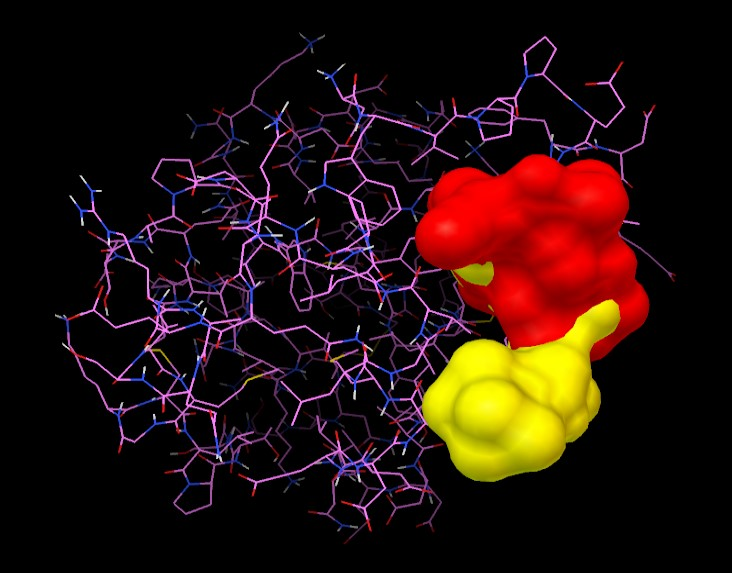
\includegraphics[width=\textwidth, height=6cm]{images/chapter4/visualization/2h8v_acrinathrin.jpg}
        \caption[]%
        {{\small Acrinathrin}}    
        \label{fig:2h8v_acrinathrin}
    \end{subfigure}
    \hfill
    \begin{subfigure}[b]{0.475\textwidth}  
        \centering 
        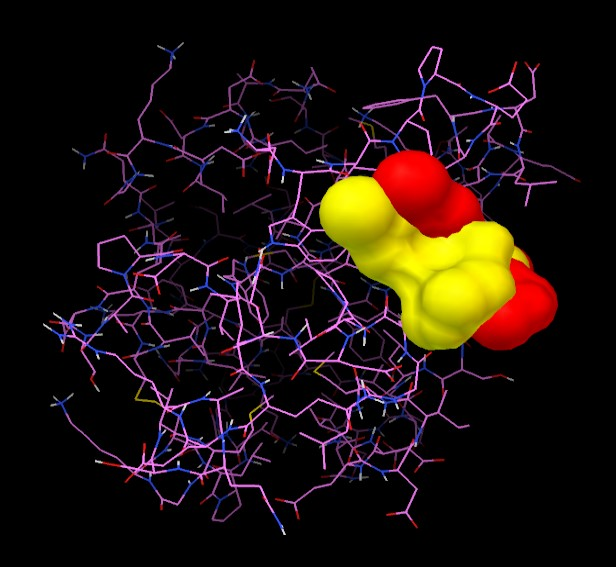
\includegraphics[width=\textwidth, height=6cm]{images/chapter4/visualization/2h8v_dimethomorph.jpg}
        \caption[]%
        {{\small Dimethomorph}}    
        \label{fig:2h8v_dimethomorph}
    \end{subfigure}
    \vskip\baselineskip
    \begin{subfigure}[b]{0.475\textwidth}   
        \centering 
        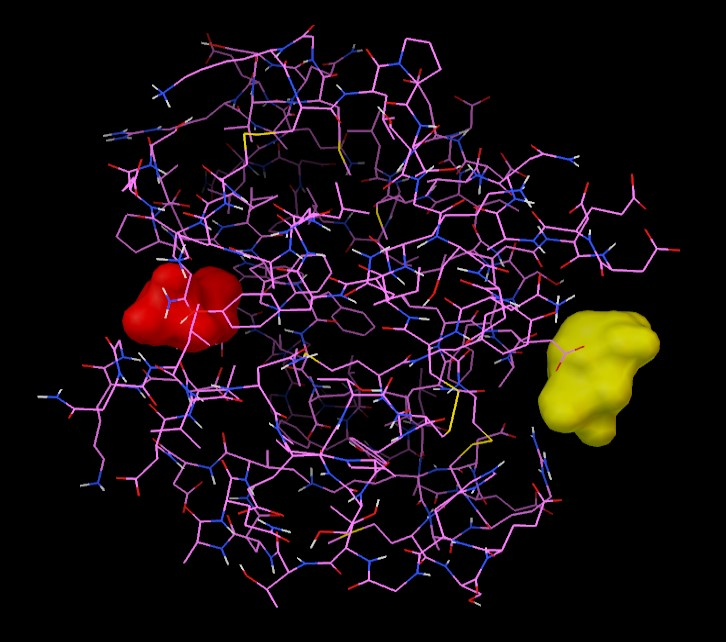
\includegraphics[width=\textwidth, height=6cm]{images/chapter4/visualization/2h8v_glyphosate.jpg}
        \caption[]%
        {{\small Glyphosate}}    
        \label{fig:2h8v_glyphosate}
    \end{subfigure}
    \hfill
    \begin{subfigure}[b]{0.475\textwidth}   
        \centering 
        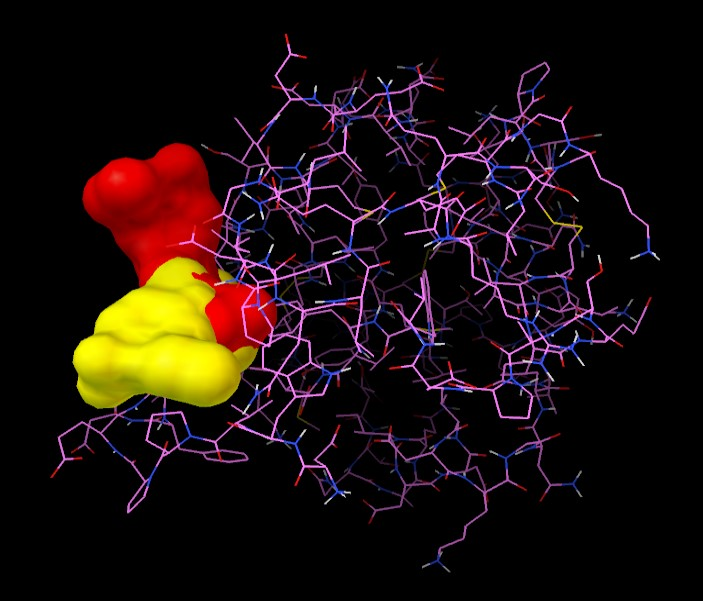
\includegraphics[width=\textwidth, height=6cm]{images/chapter4/visualization/2h8v_oxyfluorfen.jpg}
        \caption[]%
        {{\small Oxyfluorfen}}    
        \label{fig:2h8v_oxyfluorfen}
    \end{subfigure}
    \caption[Conformazioni proteina-ligando per la proteina 2H8V]
    {\small Visualizzazione delle migliori pose generate da GNINA (in giallo) ed AutoDock Vina (in rosso) relativamente alla proteina 2H8V ed alcuni dei ligandi del dataset iniziale (Acrinathrin, Dimethomorph, Glyphosate, Oxyfluorfen).} 
    \label{fig:2h8v}
\end{figure}

A partire dalla Figura \ref{fig:2h8v}, è possibile notare come, per una proteina di modeste dimensioni, tendenzialmente il sito di legame relativo alle migliori pose predette è circa lo stesso, a meno di orientazioni e torsioni del ligando coinvolto, risultando predizioni piuttosto simili tra i software, sebbene configurati per scopi diversi.


\begin{figure}
    \centering
    \begin{subfigure}[b]{0.475\textwidth}
        \centering
        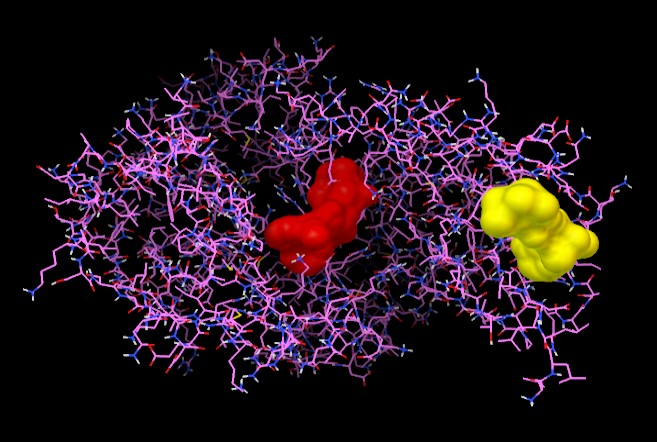
\includegraphics[width=\textwidth, height=6cm]{images/chapter4/visualization/4e81_acrinathrin.jpg}
        \caption[]%
        {{\small Acrinathrin}}    
        \label{fig:2h8v_acrinathrin}
    \end{subfigure}
    \hfill
    \begin{subfigure}[b]{0.475\textwidth}  
        \centering 
        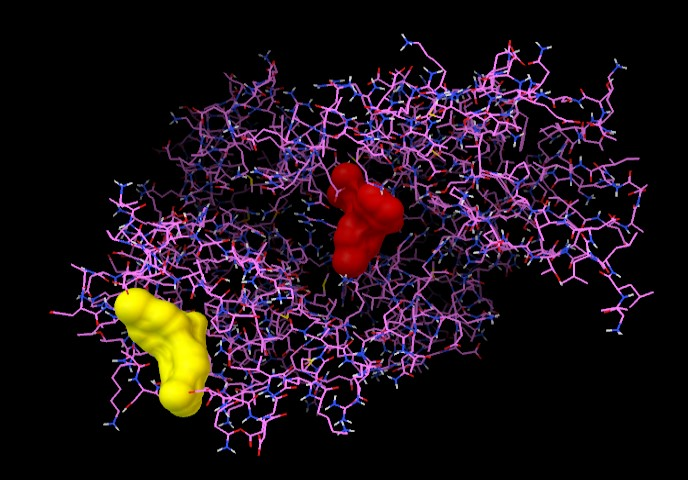
\includegraphics[width=\textwidth, height=6cm]{images/chapter4/visualization/4e81_dimethomorph.jpg}
        \caption[]%
        {{\small Dimethomorph}}    
        \label{fig:2h8v_dimethomorph}
    \end{subfigure}
    \vskip\baselineskip
    \begin{subfigure}[b]{0.475\textwidth}   
        \centering 
        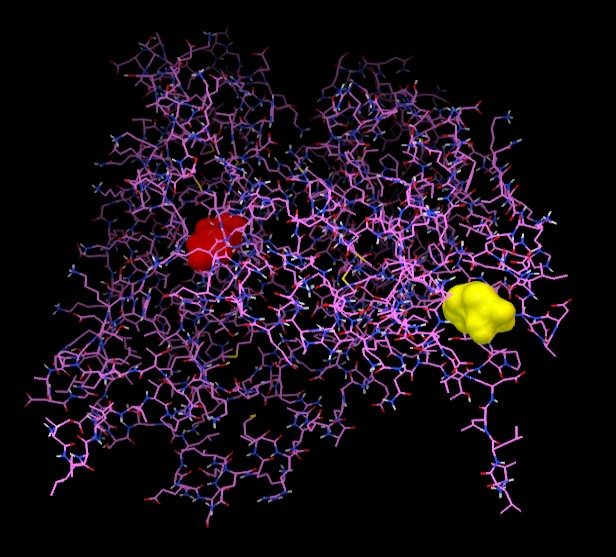
\includegraphics[width=\textwidth, height=6cm]{images/chapter4/visualization/4e81_glyphosate.jpg}
        \caption[]%
        {{\small Glyphosate}}    
        \label{fig:2h8v_glyphosate}
    \end{subfigure}
    \hfill
    \begin{subfigure}[b]{0.475\textwidth}   
        \centering 
        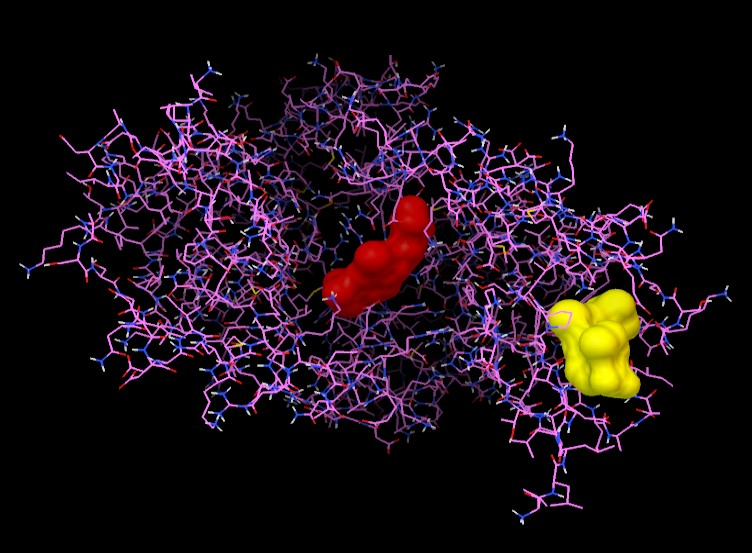
\includegraphics[width=\textwidth, height=6cm]{images/chapter4/visualization/4e81_oxyfluorfen.jpg}
        \caption[]%
        {{\small Oxyfluorfen}}    
        \label{fig:2h8v_oxyfluorfen}
    \end{subfigure}
    \caption[Conformazioni proteina-ligando per la proteina 4E81. ]
    {\small Visualizzazione delle migliori pose generate da GNINA (in giallo) ed AutoDock Vina (in rosso) relativamente alla proteina 4E81 ed alcuni dei ligandi del dataset iniziale (Acrinathrin, Dimethomorph, Glyphosate, Oxyfluorfen).} 
    \label{fig:4e81}
\end{figure}



Le cose si fanno interessanti invece se osserviamo una proteina di dimensioni maggiori rispetto alla precedente. La Figura \ref{fig:4e81} mostra la notevole differenza nelle predizioni: nel caso di GNINA, il ligando risulta occupare una posizione quasi esterna alla proteina mentre è tendenzialmente interna nel caso di AutoDock Vina. E' ipotizzabile che questa situazione sia condizionata dalla struttura molecolare della proteina coinvolta, tuttavia è comunque una differenza rispetto a strutture proteiche di questo genere.


\begin{figure}[H]
    \centering
    \begin{subfigure}[b]{0.475\textwidth}
        \centering
        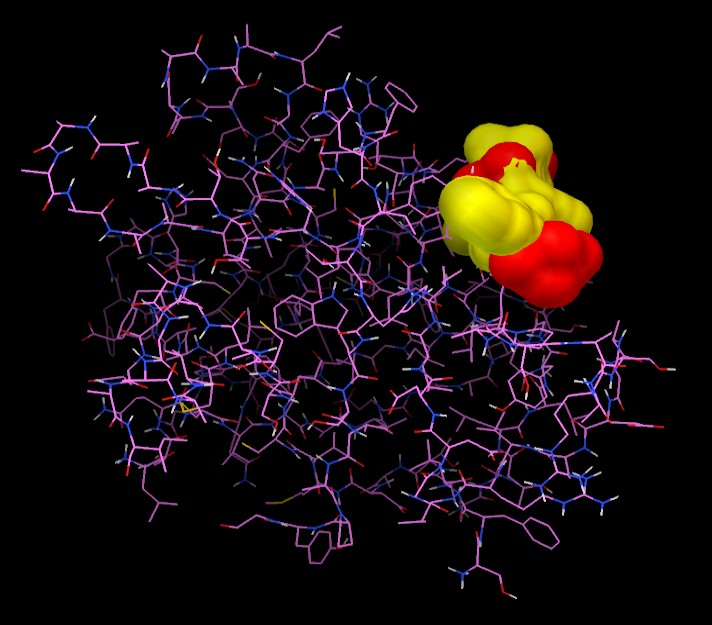
\includegraphics[width=\textwidth, height=6cm]{images/chapter4/visualization/6lqk_b_acrinathrin.jpg}
        \caption[]%
        {{\small Acrinathrin}}    
        \label{fig:2h8v_acrinathrin}
    \end{subfigure}
    \hfill
    \begin{subfigure}[b]{0.475\textwidth}  
        \centering 
        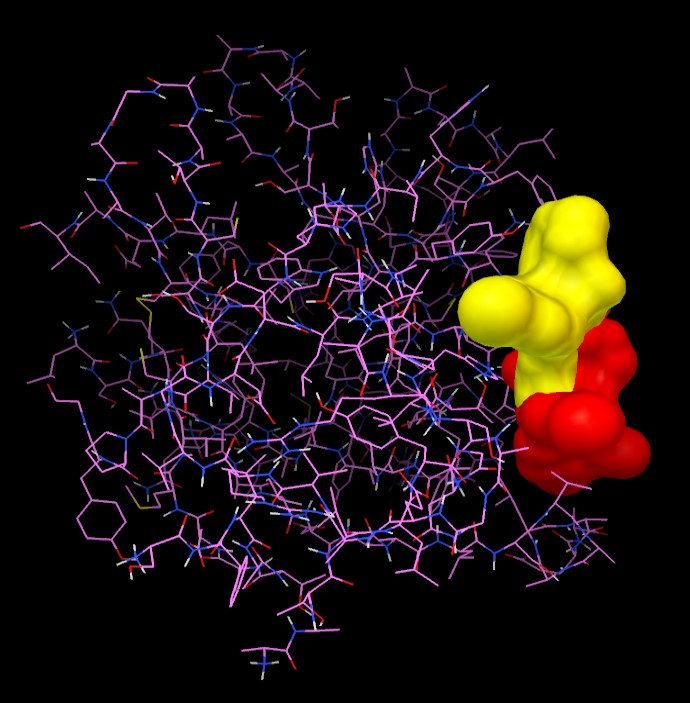
\includegraphics[width=\textwidth, height=6cm]{images/chapter4/visualization/6lqk_b_dimethomorph.jpg}
        \caption[]%
        {{\small Dimethomorph}}    
        \label{fig:2h8v_dimethomorph}
    \end{subfigure}
    \vskip\baselineskip
    \begin{subfigure}[b]{0.475\textwidth}   
        \centering 
        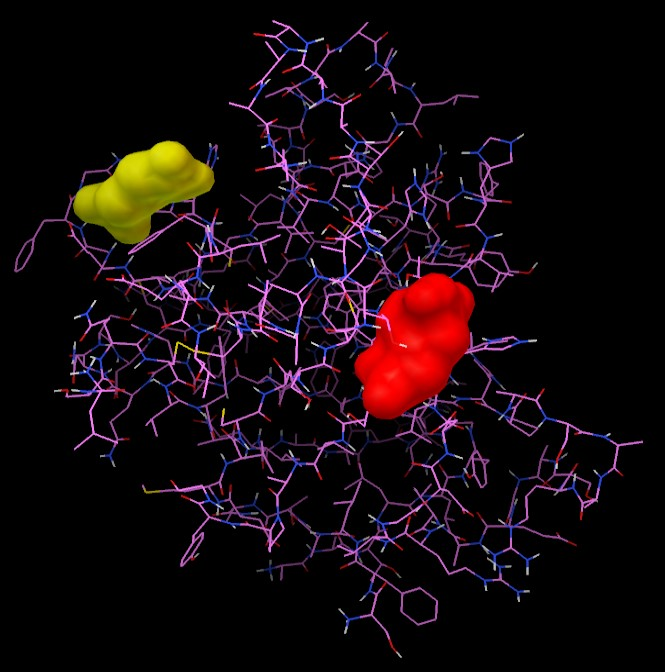
\includegraphics[width=\textwidth, height=6cm]{images/chapter4/visualization/6lqk_b_glyphosate.jpg}
        \caption[]%
        {{\small Glyphosate}}    
        \label{fig:2h8v_glyphosate}
    \end{subfigure}
    \hfill
    \begin{subfigure}[b]{0.475\textwidth}   
        \centering 
        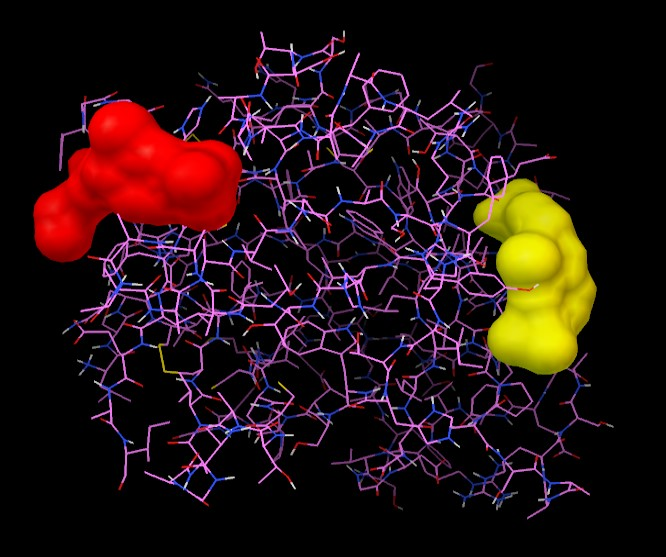
\includegraphics[width=\textwidth, height=6cm]{images/chapter4/visualization/6lqk_b_oxyfluorfen.jpg}
        \caption[]%
        {{\small Oxyfluorfen}}    
        \label{fig:2h8v_oxyfluorfen}
        \end{subfigure}
    \caption[Conformazioni proteina-ligando per la proteina 6LQK\_B. ]
    {\small Visualizzazione delle migliori pose generate da GNINA (in giallo) ed AutoDock Vina (in rosso) relativamente alla proteina 6LQK\_B ed alcuni dei ligandi del dataset iniziale (Acrinathrin, Dimethomorph, Glyphosate, Oxyfluorfen).} 
    \label{fig:6lqk_b}
\end{figure}

L'ultima visualizzazione riguarda la proteina più grande delle tre sopracitate ossia la 6LQK\_B. La Figura \ref{fig:6lqk_b} mostra come coesistono situazioni in cui la predizione è circa la stessa ed altre in cui è nettamente differente.
Tuttavia, è possibile notare come prevalentemente le pose predette siano esterne. Il motivo di questo può essere dovuto al fatto che la struttura proteica in questione non presenta cavità per legami interni coi ligandi.


Ricordo ovviamente che la riproducibilità di una certo esperimento di docking è possibile se e soltanto se il seme pseudo-casuale per ciascun software è impostato ad un valore costante. 
\section{Minimized Symmetric-Corrected RMSD}
Come introdotto nella Sezione \ref{mscrmsd}, per valutare la distanza tra la posa cristallizzata del ligando naturale e la posa predetta del ligando è stata utilizzata la Minimized Symmetric-Corrected RMSD.
Da qui in avanti per RMSD s'intende la versione minimizzata della RMSD con correzione della simmetria.

Quindi, per ogni molecola del ligando di ciascuna coppia proteina-ligando è stata calcolata la RMSD. Rispetto all'insieme delle RMSD per le molecole, ne viene calcolata la media per ottenere la RMSD della coppia proteina-ligando. Successivamente, è stata calcolato il valore medio della RMSD per la proteina, considerando ciascuna delle coppie proteina-ligando. Questo ha permesso di valutare le prestazioni del software GNINA in termini di RMSD delle pose predette. 

Le RMSD medie sono riportate in tabella per ciascuna delle proteine selezionate dal dataset iniziale. Inoltre, viene affiancata la magnitudo della differenza, che fornisce una misura della distanza tra i valori medi calcolati in funzione delle pose predette da ciascun software; in particolare, la magnitudo è negativa quando il valore medio della RMSD di GNINA calcolato è inferiore rispetto a quello di AutoDock Vina. Viceversa, una magnitudo positiva indica una prestazione peggiore in termini di RMSD media calcolata da parte di GNINA su AutoDock Vina. 

\begin{table}[H] 
\centering
\resizebox{0.8\columnwidth}{!}{%
\begin{tabular}{cccc}
\toprule
\textbf{\begin{tabular}[c]{@{}@{}c@{}}Protein\\ (code)\end{tabular}}      & \textbf{\begin{tabular}[c]{@{}@{}c@{}}AutoDock Vina\\ Average RMSD\\ (Angstroms)\end{tabular}} & \textbf{\begin{tabular}[c]{@{}@{}c@{}}GNINA\\ Average RMSD\\ (Angstroms)\end{tabular}} & \textbf{\begin{tabular}[c]{@{}@{}c@{}}Magnitude\\ (scalar)\end{tabular}}              \\ \midrule
1FCU                   & 1.382                                                                         & 1.330                                                                 & \(\textbf{-}5.2 \cdot 10^{-2}\) \\ \midrule
2H8V                   & 1.396                                                                         & 1.368                                                                 & \(\textbf{-}2.8 \cdot 10^{-2}\) \\ \midrule
3FE9                   & 0.015                                                                         & 0.013                                                                 & \(\textbf{-}1.5 \cdot 10^{-3}\) \\ \midrule
4E81                   & 1.365                                                                         & 1.346                                                                 & \(\textbf{-}1.9 \cdot 10^{-2}\) \\ \midrule
5XZ3\_A                & 1.394                                                                         & 1.358                                                                 & \(\textbf{-}3.6 \cdot 10^{-2}\) \\ \midrule
6LQK\_B                & 1.350                                                                         & 1.363                                                                 & \(1.3 \cdot 10^{-2}\)           \\ \midrule
\multicolumn{1}{l}{} & 1.150                                                                         & 1.130                                                                 & \(\textbf{-}2.1 \cdot 10^{-2}\) \\ \bottomrule
\end{tabular}%
}
\caption[Valori medi di RMSD* e magnitudo della differenza risultanti dalle pose predette da GNINA ed AutoDock Vina.]
{\small Valori medi di Minimized Symmetric-Corrected RMSD risultanti dalle pose predette da GNINA ed AutoDock Vina, affiancati dall'ordine di grandezza o magnitudo della differenza tra i valori medi dei rispettivi software. Nell'ultima riga sono riportati rispettivamente la media delle medie delle RMSD per AutoDock Vina e GNINA, ed il valore medio della magnitudo.}
\label{rmsd_table}
\end{table}

Come si evince dalla Tabella \ref{rmsd_table} e come era possibile ipotizzare, i valori della RMSD per ciascuna proteina risultano essere mediamente inferiori nel caso di GNINA, rispetto a quelli riportati da AutoDock Vina, per un ordine di grandezza pari a 2 o 3 cifre decimale, nella maggior parte dei casi d'esempio proposti (5/6).
L'ultima riga della Tabella \ref{rmsd_table} sintetizza questo andamento: generalmente GNINA risulta effettuare predizioni migliori delle pose in termini di RMSD, a partire già dalla seconda cifra decimale se confrontato con AutoDock Vina.

D'altro canto, questo tipo di situazione era ipotizzabile poiché ai fini dell'esperimento, la CNN è stata impostata per classificare le pose del ligando rispetto al parametro CNNscore, che favorisce pose con la probabilità più alta di avere un RMSD basso (vedi Sezione \ref{cnn_params}).

\section{Previsione dell'affinità}
Come descritto nella Sezione \ref{cnn_params}, l'output di GNINA distingue tre metriche differenti: CNNscore, CNNaffinity e Energy che è equivalente all'affinità di output predetta da AutoDock Vina.

Per questo motivo, è interessante valutare le prestazioni di GNINA rispetto al valore di affinità.
Ricordo che in questo esperimento, GNINA è configurato per utilizzare la rete neurale convoluzionale durante la fase di \textit{"rescore"} e che soprattutto, il ranking delle pose avviene secondo il criterio predefinito ossia secondo il parametro CNNscore.

Per questo ci aspettiamo che AutoDock Vina possa avere risultati migliori in termini di affinità predetta. 

Per ciascuna delle proteine selezionate dal dataset iniziale, sono riportati i valori medi di output corrispondenti. Oltre al valore medio di CNNscore, in ciascun caso il valore medio dell'affinità predetta da GNINA è affiancato al valore medio dell'affinità predetta da AutoDock Vina. 

\begin{table}[H] 
\centering
\resizebox{0.9\columnwidth}{!}{%
\begin{tabular}{ccccc}
\toprule
\textbf{\begin{tabular}[c]{@{}@{}c@{}}Protein\\ (code)\end{tabular}} & \textbf{\begin{tabular}[c]{@{}@{}c@{}}Average\\ CNNscore\\ (scalar)\end{tabular}} & \textbf{\begin{tabular}[c]{@{}@{}c@{}}Average\\ CNNaffinity\\ (pK)\end{tabular}} & \textbf{\begin{tabular}[c]{@{}@{}c@{}}Average\\ GNINA\\ affinity\\ (kcal/mol)\end{tabular}} & \textbf{\begin{tabular}[c]{@{}@{}c@{}}Average\\ AutoDock Vina\\ affinity\\ (kcal/mol)\end{tabular}} \\ \midrule
1FCU              & 0.654             & 4.390                                                               & -5.023                                                                         & -6.288                                                                                 \\ \midrule
2H8V              & 0.694             & 4.620                                                               & -4.895                                                                         & -5.556                                                                                 \\ \midrule
3FE9              & 0.690             & 5.571                                                               & -6.547                                                                         & -7.266                                                                                 \\ \midrule
4E81              & 0.639             & 4.689                                                               & -5.576                                                                         & -6.646                                                                                 \\ \midrule
5XZ3\_A           & 0.626             & 4.454                                                               & -5.053                                                                         & -5.963                                                                                 \\ \midrule
6LQK\_B           & 0.689             & 4.448                                                               & -4.808                                                                         & -5.518                                                                                 \\ \bottomrule
\end{tabular}%
}
\caption{Valori medi per i parametri di output di GNINA, ovvero CNNscore, CNNaffinity ed Energy (affinity), affiancati dal valore medio di affinità predetta da AutoDock Vina.}
\label{affinity_table}
\end{table}

I valori medi danno un'indicazione sulla bontà dell'applicazione della rete neurale convoluzionale. Ai fini di un'analisi di valutazione dei rischi, non consistono di una certa rilevanza ma nel caso specifico possono dare una visione più chiara delle prestazioni, soprattutto per la capacità di sintesi del valore medio di un certo andamento.  
Come si evince dalla Tabella \ref{affinity_table}, innanzitutto rispetto al set di ligandi considerato, le proteine risultano avere analiticamente e mediamente circa le stesse valutazioni. E' interessante però osservare come si comporta una CNN, modellata per massimizzare il parametro CNNscore, rispetto al parametro affinità. 
Come era possibile ipotizzare, in ciascun caso campione, GNINA riporta mediamente un valore di affinità superiore rispetto ad AutoDock Vina. 

A tal proposito, sarebbe interessante valutare come si comporta il modello CNN e quindi le prestazioni di GNINA, modificando il criterio per il ranking delle pose da CNNscore ad Energy, corrispondente all'affinità. 

\section{Rilevazione delle interazioni molecolari}
Finora le valutazioni delle prestazioni hanno evidenziato che le pose predette da GNINA risultano essere migliori in termini di RMSD  ma allo stesso tempo peggiori in termini di affinità predetta se comparate con quelle di AutoDock Vina. Ragion per cui, la rilevazione e l'analisi delle interazioni molecolari prodotte all'interno della conformazione proteina-ligando assume una notevole importanza, specie per determinare l'efficacia dell'applicazione della rete neurale in questo contesto.

A tale scopo, sono state rilevate le interazioni molecolari interessanti per ciascuna coppia proteina-ligando e poi sintetizzate graficamente per interpretare i risultati.
Nella Sezione \ref{charts} sono stati esplicati i grafici utilizzati per rappresentare l'informazione relativa alle interazioni molecolari rilevate. 

Per ciascuna delle proteine selezionate dal dataset iniziale sono riportati in tabella il numero ed il tipo delle interazioni interessanti risultanti dal processo di rilevazione sia per GNINA che per AutoDock Vina. Inoltre, viene riportato anche il rapporto tra il numero di legami ad idrogeno rispetto al numero di contatti totali, corrispondente alla somma tra il numero di close contacts ed il numero di legami ad idrogeno (HBR, Hydrogen Bonds Ratio).

\begin{equation} \label{eq:hbr}
    HBR = \frac{hydrogen\,bonds}{close\,contacts + hydrogen\,bonds}
\end{equation}


\begin{table}[H] 
\centering 
\resizebox{\columnwidth}{!}{%
\begin{tabular}{ccccccc}
\toprule
\textbf{}                                                         & \multicolumn{3}{c}{\textbf{GNINA}}                                                                                                                                                                                                                                                                          & \multicolumn{3}{c}{\textbf{AutoDock Vina}}                                                                                                                                                                                                                                                                  \\ \midrule
\textbf{\begin{tabular}[c]{@{}c@{}}Protein\\ (code)\end{tabular}} & \multicolumn{1}{c}{\textbf{\begin{tabular}[c]{@{}c@{}}Close \\ contacts\\ (int)\end{tabular}}} & \multicolumn{1}{c}{\textbf{\begin{tabular}[c]{@{}c@{}}Hydrogen \\ bonds\\ (int)\end{tabular}}} & \textbf{\begin{tabular}[c]{@{}c@{}}Hydrogen Bonds\\ Ratio\\ (float)\end{tabular}} & \multicolumn{1}{c}{\textbf{\begin{tabular}[c]{@{}c@{}}Close \\ contacts\\ (int)\end{tabular}}} & \multicolumn{1}{c}{\textbf{\begin{tabular}[c]{@{}c@{}}Hydrogen \\ bonds\\ (int)\end{tabular}}} & \textbf{\begin{tabular}[c]{@{}c@{}}Hydrogen Bonds\\ Ratio\\ (float)\end{tabular}} \\ \midrule
1FCU                                                              & \multicolumn{1}{c}{1207}                                                                                              & \multicolumn{1}{c}{137}                                                                                                & 0.101                                                                             & \multicolumn{1}{c}{1621}                                                                                              & \multicolumn{1}{c}{185}                                                                                                & 0.102                                                                             \\ \midrule
2H8V                                                              & \multicolumn{1}{c}{1112}                                                                                              & \multicolumn{1}{c}{52}                                                                                                 & 0.044                                                                             & \multicolumn{1}{c}{1267}                                                                                              & \multicolumn{1}{c}{45}                                                                                                 & 0.034                                                                             \\ \midrule
3FE9                                                              & \multicolumn{1}{c}{1497}                                                                                              & \multicolumn{1}{c}{30}                                                                                                 & 0.019                                                                             & \multicolumn{1}{c}{1684}                                                                                              & \multicolumn{1}{c}{34}                                                                                                 & 0.019                                                                             \\ \midrule
4E81                                                              & \multicolumn{1}{c}{1326}                                                                                              & \multicolumn{1}{c}{147}                                                                                                & 0.099                                                                             & \multicolumn{1}{c}{1664}                                                                                              & \multicolumn{1}{c}{125}                                                                                                & 0.069                                                                             \\ \midrule
5XZ3\_A                                                           & \multicolumn{1}{c}{1243}                                                                                              & \multicolumn{1}{c}{169}                                                                                                & 0.119                                                                             & \multicolumn{1}{c}{1472}                                                                                              & \multicolumn{1}{c}{203}                                                                                                & 0.121                                                                             \\ \midrule
6LQK\_B                                                           & \multicolumn{1}{c}{1139}                                                                                              & \multicolumn{1}{c}{119}                                                                                                & 0.094                                                                             & \multicolumn{1}{c}{1356}                                                                                              & \multicolumn{1}{c}{163}                                                                                                & 0.107                                                                             \\ \bottomrule
\end{tabular}%
}
\caption[Interazioni nel complesso proteina-ligando generato da GNINA e AutoDock Vina.]{Close contacts e legami a idrogeno prodotti da ciascuna delle proteine selezionate rispetto alle pose generate da GNINA ed AutoDock Vina. Per ciascun software e per ciascuna proteina, viene riportato l'Hydrogen Bonds Ratio, illustrato nell'Equazione \ref{eq:hbr}.}
\label{contacts_table}
\end{table}

Dalla Tabella \ref{contacts_table}, è possibile notare che tendenzialmente il numero totale di contatti rilevati è decisamente inferiore quando viene utilizzato GNINA rispetto ad AutoDock Vina. Tuttavia, andando a rapportare il numero di legami ad idrogeno rispetto alla somma dei contatti totali, notiamo che i rapporti sono circa gli stessi. Ciò significa che in proporzione, le pose generate da GNINA permettono maggiormente la formazione di legami a idrogeno. 

L'unione dell'informazione relativa al numero di ponti ad idrogeno e quella relativa all'affinità predetta ci permette di dire che, sebbene le prestazioni del modello siano peggiori in termini di affinità, in fin dei conti la qualità del legame risulta essere migliore. In altre parole, AutoDock Vina genera pose di ligandi che risultano avere un'affinità migliore ma che nel complesso recettore-ligando creano nella maggior parte dei casi interazioni meno efficaci, sebbene in quantità maggiori rispetto a GNINA. 
Questo ci consente di confermare quanto ipotizzato fin dall'inizio, ovvero che la predizione effettuata da GNINA è certamente più predittiva rispetto ad AutoDock Vina, considerando il caso di esperimenti di blind docking.
E' ipotizzabile che questo tipo di comportamento sia accentuato ed ampiamente confermato per esperimenti di docking su sacche, cavità o siti di legame specifici.

A questo punto dell'analisi vengono mostrate le heatmap più significative per dare ancora più enfasi ai risultati sperimentali ed alle considerazioni effettuate finora. Tra le varie heatmap realizzate per le proteine selezionate, risultano essere particolarmente contrastanti quelle relative alle proteine 1FCU e 5XZ3\_A. 
I tipi di legame possibili, introdotti nella Sezione \ref{charts}, sono stati codificati come segue: nessun legame (viola), close contacts (azurrino/verde) e legami a idrogeno (giallo). Sull'asse delle ordinate sono collocati i residui della proteina e sull'asse delle ascisse sono collocati i ligandi coinvolti.  


\begin{figure}
    \centering
    \begin{subfigure}[b]{\textwidth}
        \centering
        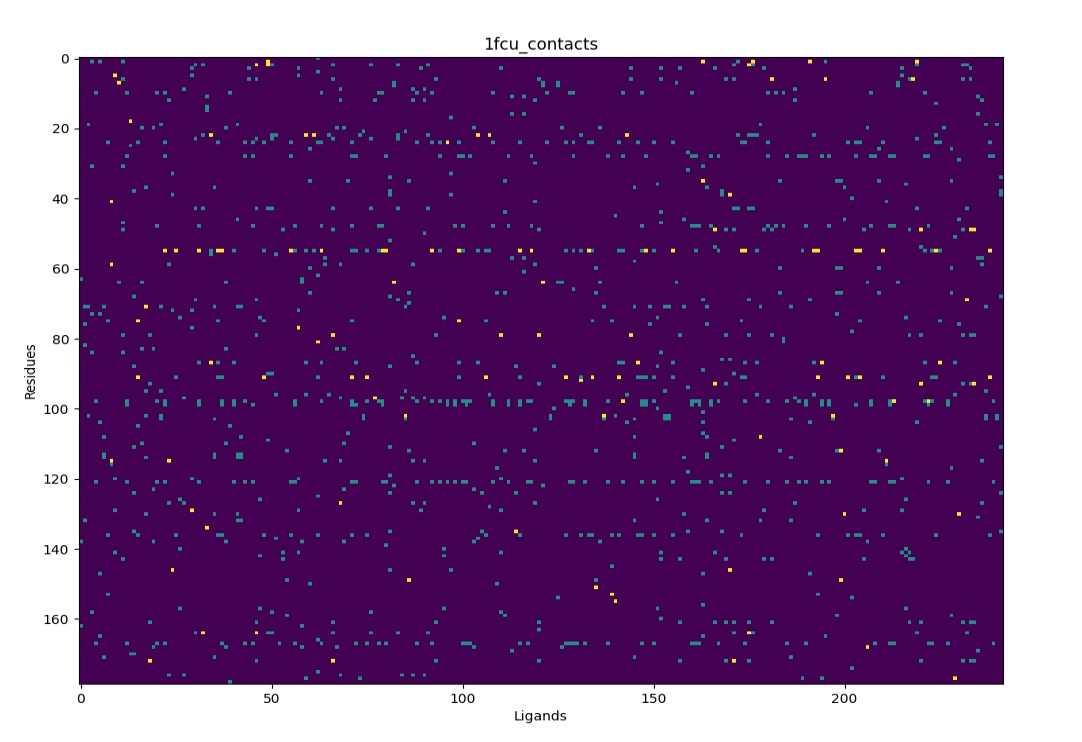
\includegraphics[width=\textwidth, height=6cm]{images/chapter4/heatmaps/heatmap_gnina_1fcu.jpg}
        \caption[]%
        {{\small Heatmap delle interazioni per la proteina 1FCU prodotta a partire dalle pose predette dei ligandi da GNINA.}}    
        \label{fig:heatmap_gnina_1fcu}
    \end{subfigure}
    \hfill
    \begin{subfigure}[b]{\textwidth}  
        \centering 
        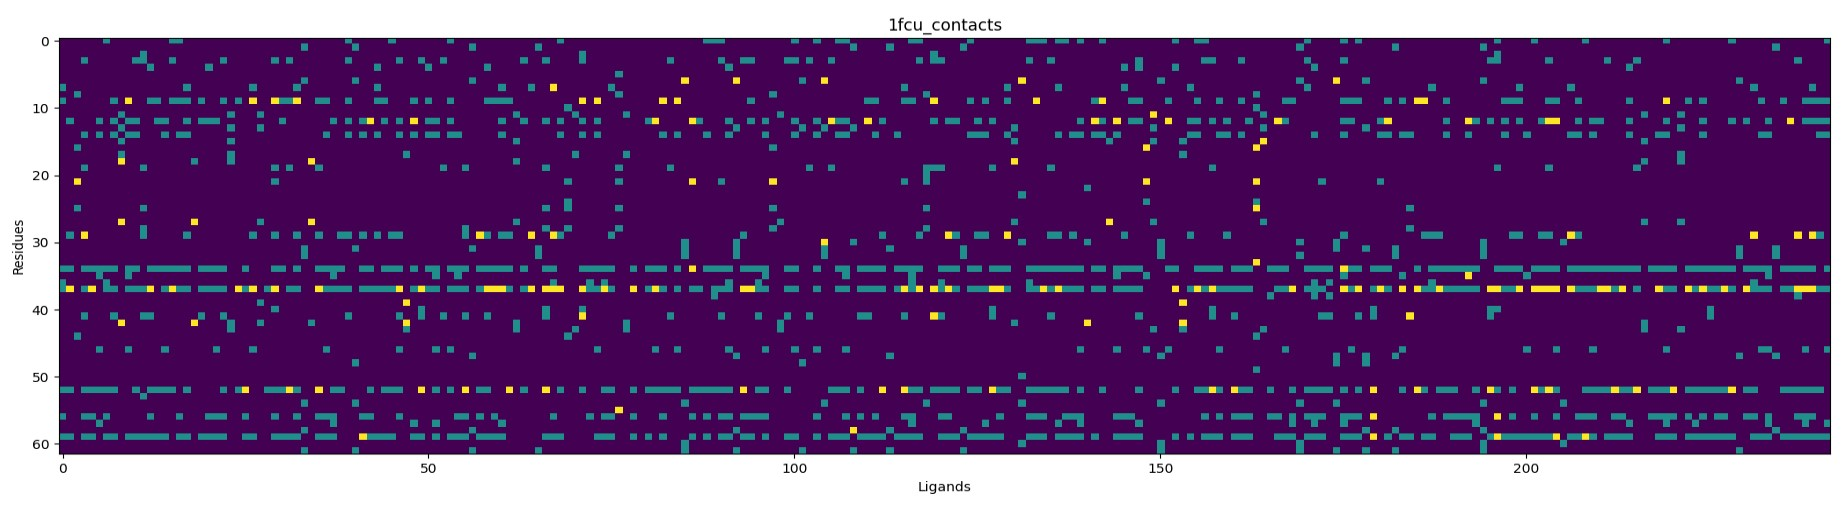
\includegraphics[width=0.9\textwidth, height=6cm]{images/chapter4/heatmaps/heatmap_vina_1fcu.jpg}
        \caption[]%
        {{\small Heatmap delle interazioni per la proteina 1FCU prodotta a partire dalle pose predette dei ligandi da AutoDock Vina.}}    
        \label{fig:heatmap_vina_1fcu}
    \end{subfigure}
    \caption[Visualizzazione delle heatmaps per la proteina 1FCU.]
    {\small Visualizzazione delle interazioni per la proteina 1FCU attraverso heatmaps. In alto, è riportata l'heatmap risultante dalle pose predette da GNINA mentre in basso, quella risultante dalle pose predette da AutoDock Vina. Sull'asse delle ascisse sono riportati i ligandi, sulle ordinate i residui coinvolti per la proteina. In giallo sono riportati i legami a idrogeno, in azzurro/verde i close contacts, in viola nessun legame. } 
    \label{fig:1fcu}
\end{figure}
 
La Figura \ref{fig:1fcu} riporta le heatmaps prodotte dall'analisi delle interazioni molecolari relativamente alla proteina 1FCU per il dataset dei ligandi utilizzato (vedi Figura \ref{fig:heatmap_gnina_1fcu} per GNINA, vedi \ref{fig:heatmap_vina_1fcu} per AutoDock Vina).

Sebbene proteine e ligandi siano processati pedissecuamente e forniti in input ai due software, come già anticipato dalla Tabella \ref{contacts_table} in termini qualitativi e quantitativi, le interazioni molecolari prodotte all'interno del complesso sono profondamente diverse. La visualizzazione delle heatmaps permette una conferma di quanto detto. 
Analizzando la Figura \ref{fig:heatmap_gnina_1fcu} che è relativa ai risultati di GNINA, è possibile notare come i residui coinvolti nell'intero processo superino le 100 unità, presentando inoltre una distribuzione più equa dei legami all'interno del complesso. Infatti, risulta impensabile cercare di sintetizzare le interazioni molecolari per la proteina 1FCU semplicemente attraverso un sotto-insieme di residui che la compongono.

La situazione è completamente diversa nel caso dei risultati di AutoDock Vina: in primo luogo, poiché il numero di residui coinvolti è pari a circa 60 unità; in secondo luogo, nell'heatmap stessa, sebbene le interazioni siano maggiori in numero,  queste sono maggiormente concentrate in determinati residui (ARG244, SER225, TYR188, TYR190). In altre parole, se nel caso di GNINA, ciascun residuo fornisce il proprio contributo in termini di interazioni, nel caso di AutoDock Vina, siamo in grado di discernere dall'insieme dei residui coinvolti, i residui che forniscono l'apporto maggiore al numero di interazioni e quelli che invece hanno un contributo minimo. Questo tipo di considerazione può essere interessante per traslare l'analisi in siti proteici specifici, ovvero quelli in cui risiedono i residui principali, piuttosto che di blind docking come nel nostro caso.

Questo tipo di situazione appare ancora più netta nel caso della proteina 5XZ3\_A, prendendo visione della Figura \ref{fig:5xz3_a}. 

\begin{figure}
    \centering
    \begin{subfigure}[b]{\textwidth}
        \centering
        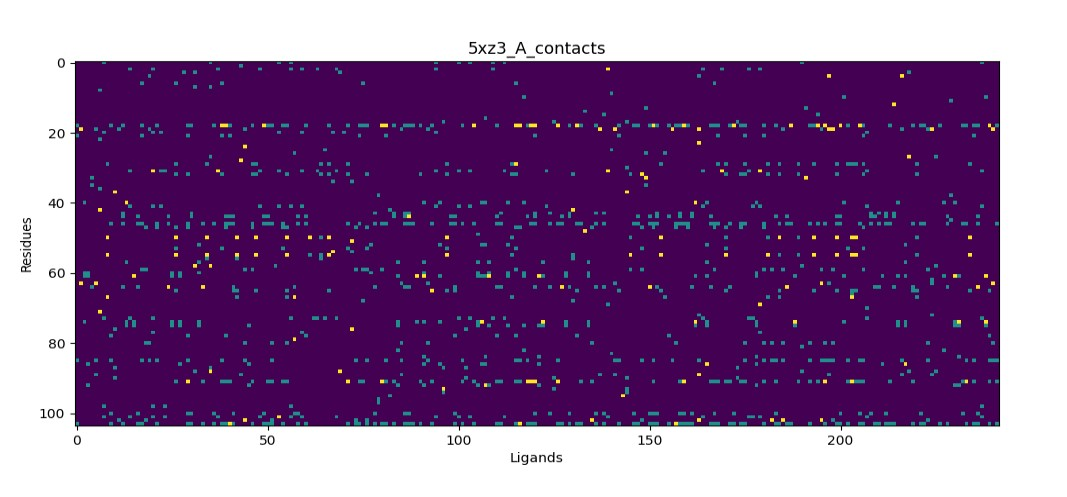
\includegraphics[width=\textwidth, height=6cm]{images/chapter4/heatmaps/heatmap_gnina_5xz3_a.jpg}
        \caption[]%
        {{\small Heatmap delle interazioni per la proteina 5XZ3\_A prodotta a partire dalle pose predette dei ligandi da GNINA.}}    
        \label{fig:heatmap_gnina_5xz3_a}
    \end{subfigure}
    \hfill
    \begin{subfigure}[b]{\textwidth}  
        \centering 
        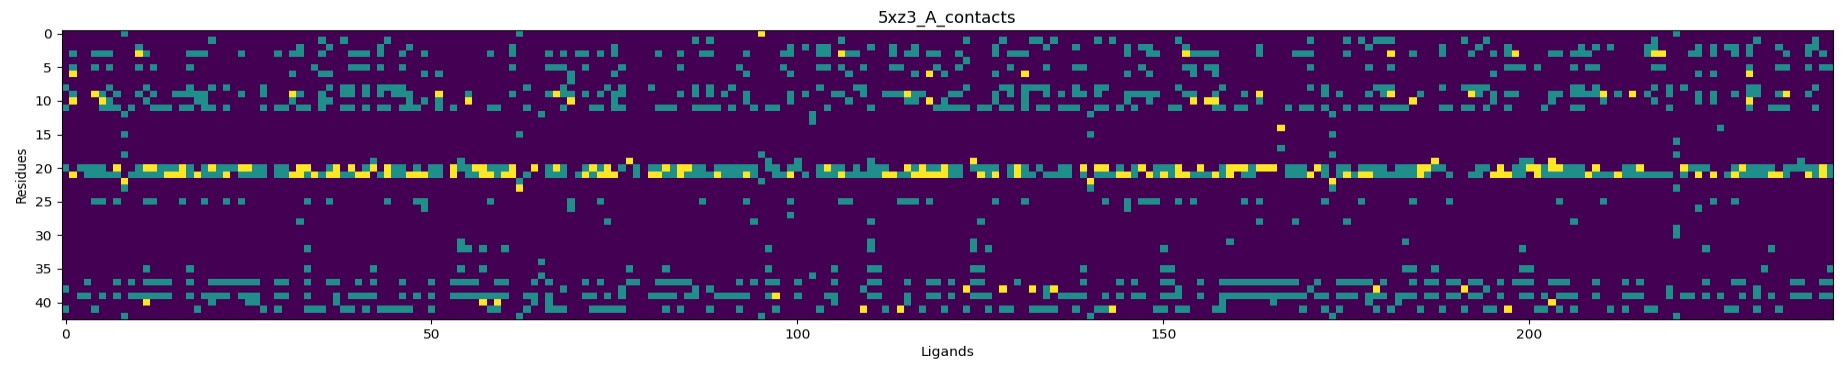
\includegraphics[width=0.9\textwidth, height=3cm]{images/chapter4/heatmaps/heatmap_vina_5xz3_a.jpg}
        \caption[]%
        {{\small Heatmap delle interazioni per la proteina 5XZ3\_A prodotta a partire dalle pose predette dei ligandi da AutoDock Vina.}}    
        \label{fig:heatmap_vina_5xz3_a}
    \end{subfigure}
    \caption[Visualizzazione delle heatmaps per la proteina 5XZ3\_A.]
    {\small Visualizzazione delle interazioni per la proteina 5XZ3\_A attraverso heatmaps. In alto, è riportata l'heatmap risultante dalle pose predette da GNINA mentre in basso, quella risultante dalle pose predette da AutoDock Vina. Sull'asse delle ascisse sono riportati i ligandi, sulle ordinate i residui coinvolti per la proteina. In giallo sono riportati i legami a idrogeno, in azzurro/verde i close contacts, in viola nessun legame. } 
    \label{fig:5xz3_a}
\end{figure}

In questo caso però, la particolarità delle relative heatmaps sta nel fatto che nel caso della Figura \ref{fig:heatmap_vina_5xz3_a}, corrispondente ai risultati di AutoDock Vina, è possibile sintetizzare non solo la maggior parte delle interazioni in un sotto-insieme dei residui coinvolti, comunque minore in numero rispetto a quello evidenziato dalla Figura \ref{fig:heatmap_gnina_5xz3_a} relativa ai risultati di GNINA, ma anche la maggior parte dei legami a idrogeno prodotti in un sotto-insieme ancor più ridotto dei residui che compongono la proteina (HIS61, TYR72).

Sebbene le considerazioni siano plausibili nel caso di AutoDock Vina, rispetto al caso di GNINA queste sono totalmente insignificanti.

Le medesime considerazioni possono essere fatte ancor più intuitivamente visualizzando gli istogrammi relativi alle interazioni prodotte, i cui picchi individuano i residui maggiormente presenti nei legami. In basso sono riportati i residui che effettuano almeno un'interazione rilevanti; in blu è riportato il numero di close contacts mentre in arancione il numero di legami a idrogeno per ciascun residuo proteico.

\begin{figure}
    \centering
    \begin{subfigure}[b]{\textwidth}
        \centering
        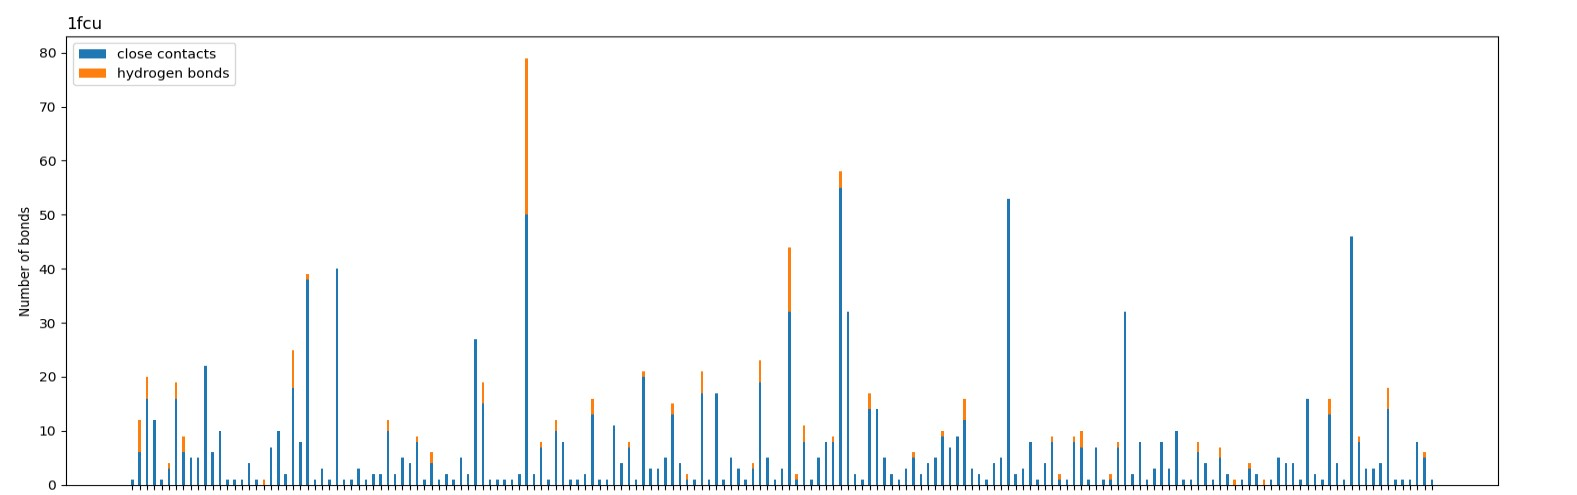
\includegraphics[width=\textwidth, height=6cm]{images/chapter4/interactions/interactions_gnina_1fcu.jpg}
        \caption[]%
        {{\small Heatmap delle interazioni per la proteina 5XZ3\_A prodotta a partire dalle pose predette dei ligandi da GNINA.}}    
        \label{fig:interactions_gnina_1fcu}
    \end{subfigure}
    \hfill
    \begin{subfigure}[b]{\textwidth}  
        \centering 
        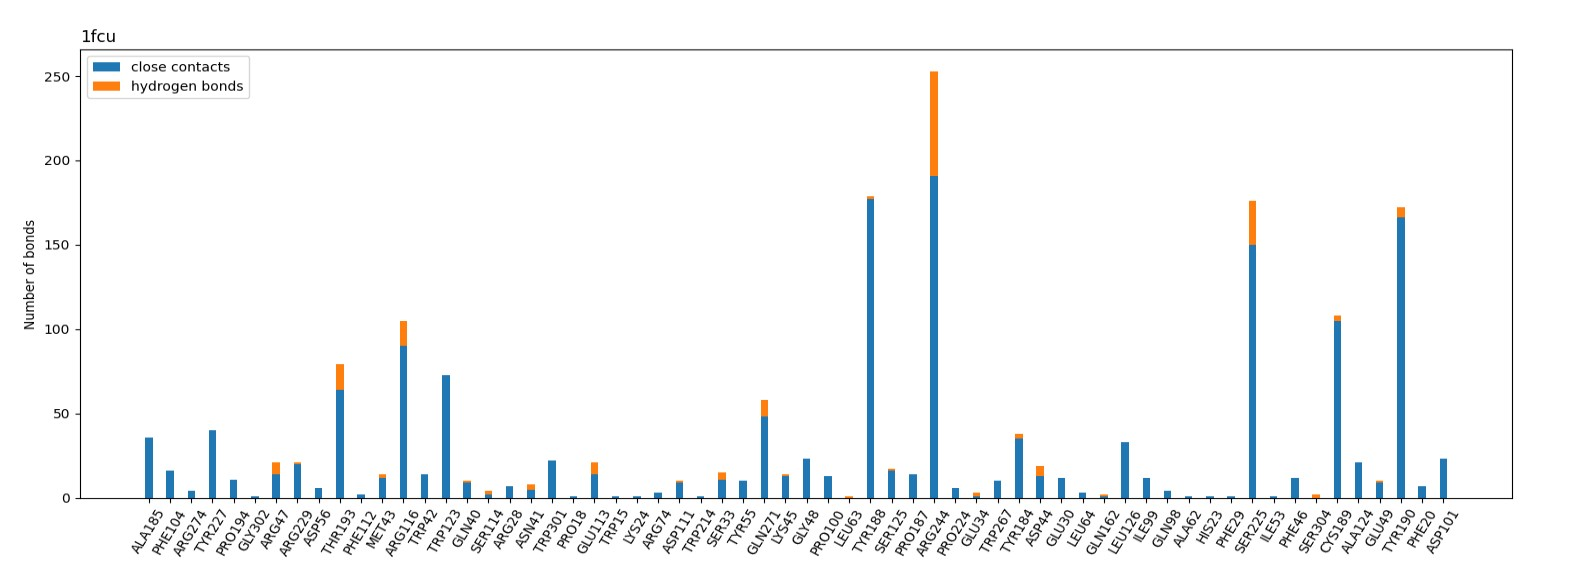
\includegraphics[width=0.9\textwidth, height=3cm]{images/chapter4/interactions/interactions_vina_1fcu.jpg}
        \caption[]%
        {{\small Istogramma delle interazioni per la proteina 1FCU prodotta a partire dalle pose predette dei ligandi da AutoDock Vina.}}    
        \label{fig:interactions_vina_1fcu}
    \end{subfigure}
    \caption[Visualizzazione degli istogrammi per la proteina 1FCU.]
    {\small Visualizzazione delle interazioni per la proteina 1FCU attraverso istogrammi. In alto, è riportato l'istogramma risultante dalle pose predette da GNINA mentre in basso, quello risultante dalle pose predette da AutoDock Vina. Sull'asse delle ordinate è riportato il numero di contatti, sulle ascisse i residui coinvolti per ciascuna proteina. In arancione sono riportati i legami a idrogeno, in blu i close contacts. } 
    \label{fig:int_1fcu}
\end{figure}


\begin{figure}
    \centering
    \begin{subfigure}[b]{\textwidth}
        \centering
        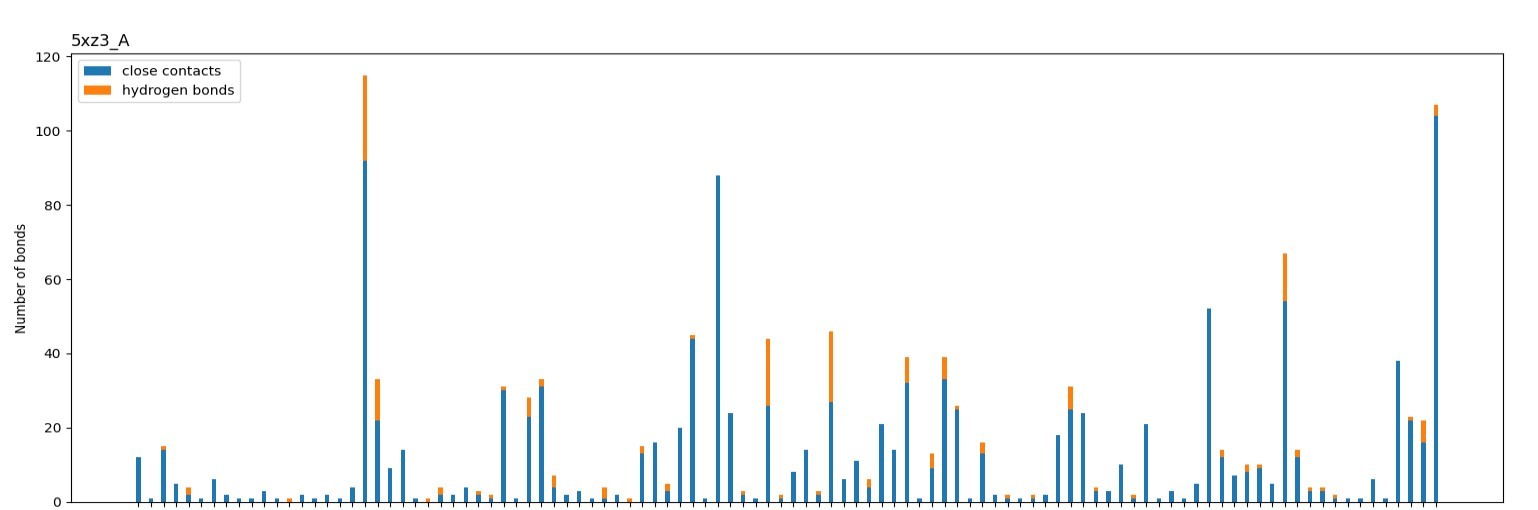
\includegraphics[width=\textwidth, height=6cm]{images/chapter4/interactions/interactions_gnina_5xz3_a.jpg}
        \caption[]%
        {{\small Istogramma delle interazioni per la proteina 5XZ3\_A prodotta a partire dalle pose predette dei ligandi da GNINA.}}    
        \label{fig:interactions_gnina_5xz3_a}
    \end{subfigure}
    \hfill
    \begin{subfigure}[b]{\textwidth}  
        \centering 
        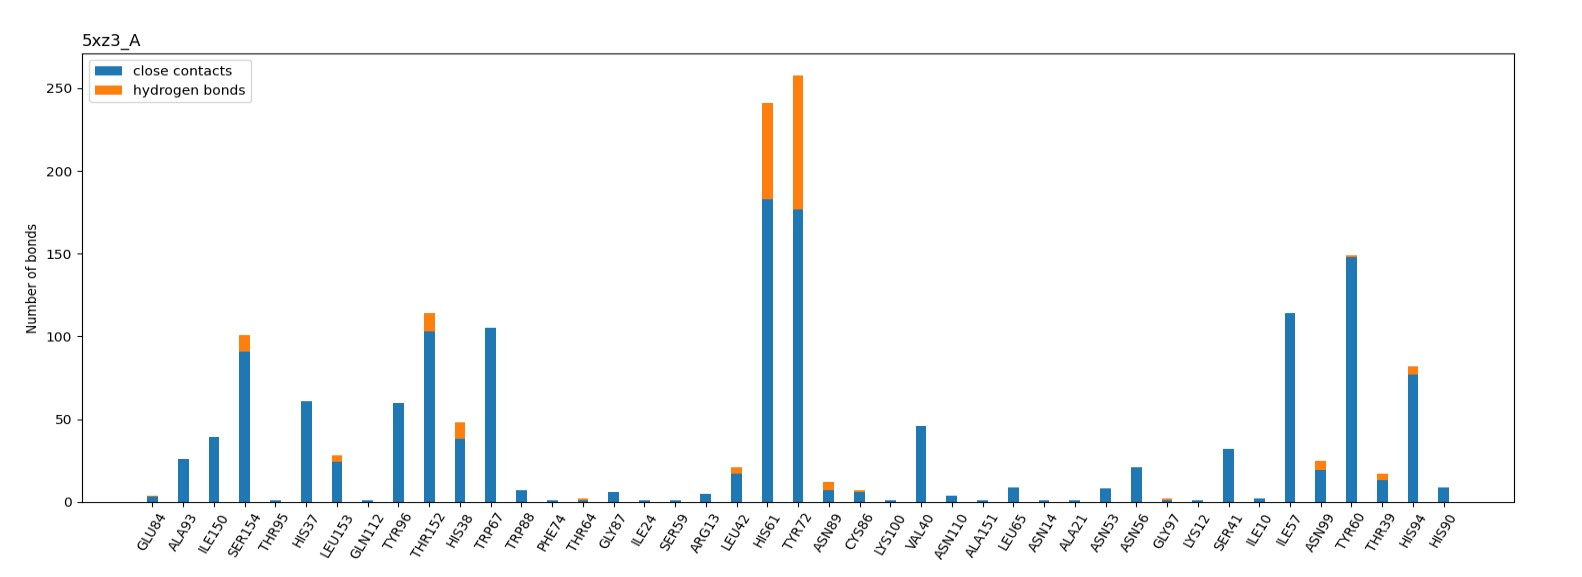
\includegraphics[width=0.9\textwidth, height=3cm]{images/chapter4/interactions/interactions_vina_5xz3_a.jpg}
        \caption[]%
        {{\small Istogramma delle interazioni per la proteina 5XZ3\_A prodotta a partire dalle pose predette dei ligandi da AutoDock Vina.}}    
        \label{fig:interactions_vina_5xz3_a}
    \end{subfigure}
    \caption[Visualizzazione degli istogrammi per la proteina 5XZ3\_A.]
    {\small Visualizzazione delle interazioni per la proteina 5XZ3\_A attraverso istogrammi. In alto, è riportato l'istogramma risultante dalle pose predette da GNINA mentre in basso, quello risultante dalle pose predette da AutoDock Vina. Sull'asse delle ordinate è riportato il numero di contatti, sulle ascisse i residui coinvolti per ciascuna proteina. In arancione sono riportati i legami a idrogeno, in blu i close contacts.} 
    \label{fig:int_5xz3_a}
\end{figure}

Mettendo insieme queste considerazioni, assieme a quelle fatte in precedenza all'interno di questo capitolo, siamo in grado di affermare che le prestazioni della rete neurale convoluzionale applicata all'interno di GNINA danno luogo a risultati estremamente diversi rispetto a quelli forniti da un software tradizionalmente usato per analisi di blind docking. 
In particolare, dall'analisi dei risultati sperimentali emerge che le predizioni effettuate da GNINA risultano essere migliori in termini di RMSD (vedi Tabella \ref{rmsd_table}) ma peggiori in termini di affinità (vedi Tabella \ref{affinity_table}). Dal punto di vista delle interazioni molecolari nel complesso però è stato dimostrato che, sebbene siano quantitativamente inferiori, queste siano qualitativamente migliori, come testimonia la parità rispetto all'Hydrogen Bonds Ratio (vedi Tabella \ref{contacts_table}).

Ciò significa che una bassa RMSD non implica necessariamente un'affinità migliore e che un'affinità migliore non implica necessariamente legami più stabili ed efficaci. 

Nonostante il numero di legami sia inferiore, è emerso che il numero di residui coinvolti in legami è notevolmente maggiore, producendo quindi heatmaps più ampie e sparse in cui le interazioni sono maggiormente distribuite, rispetto a quelle ridotte e fitte di AutoDock Vina, in cui è maggiormente possibile approssimare l'insieme dei residui coinvolti in interazioni ad un sotto-insieme ridotto di residui interessanti.



\section{Considerazioni sui tempi del docking}
La durata dell'intero processo di docking è estremamente lunga ed è influenzata dalla dimensione del dataset iniziale che si vuole analizzare e dalle risorse a disposizione. Nonostante lo sfruttamento di ambienti di calcolo parallelo, rimane comunque un'operazione onerosa sia dal punto di vista computazionale sia in termini di risorse impiegate. 

L'utilizzo della rete neurale convoluzionale costringe all'impiego di moderne risorse hardware per compiere il processo di docking sottoposto. 
Ragion per cui, è necessaria almeno una moderna GPU NVIDIA con 4 o più GB di RAM per avere risultati in tempi moderati \cite{mcnutt_gnina_2021}. 

Per l'ottenimento dei risultati relativi alle proteine selezionate, sono state necessarie in media circa 3 ore, sfruttando le potenze di calcolo messe a disposizione da Google Colab. 
In generale l'ottenimento dei risultati per entrambi i software ha richiesto circa lo stesso tempo; tuttavia, nel caso di GNINA, sono state utilizzate risorse hardware importanti, rappresentando un aspetto da non trascurare assolutamente nella scelta del software di docking per l'analisi che si vuole effettuare. Il tempo impiegato dal software, e quindi dall'applicazione delle rete neurale convoluzionale all'interno del processo di docking, e la necessità di una potenza di calcolo modesta rappresentano le maggiori criticità dell'approccio avanzato. L'elaborato è la dimostrazione di come grazie al 
\textbf{cloud computing} sia possibile, in parte, far fronte a tali criticità.


\thispagestyle{plain}
\markboth{\large{CONCLUSIONI}}{\large{CONCLUSIONI}}
\addcontentsline{toc}{chapter}{Conclusioni}
\chapter*{Conclusioni}
\noindent L'obiettivo della tesi è l'illustrazione di un approccio avanzato per l'analisi delle interazioni molecolari nell'ambito del docking computazionale. L'approccio avanzato proviene dal Deep Learning, una branca dell'Intelligenza Artificiale, nella quale le reti neurali convoluzionali, dopo una fase di apprendimento in cui estraggono da sé le caratteristiche rilevanti della conformazione proteina-ligando, effettuano una predizione sulla miglior posa del ligando secondo particolari metriche, tenendo conto di alcune limitazioni come la rigidità delle strutture, ed effettuano valutazioni energetiche a partire da tale conformazione. 
Le valutazione delle prestazioni della rete neurale convoluzionale applicata al docking computazionale non è abbastanza efficace se non è introdotto un termine di paragone, che riesca a fornire profondità allo studio di questo approccio avanzato. A tal proposito, è stato selezionato un tradizionale software di docking computazionale, basato su un approccio empirico, spesso utilizzato in analisi di questo genere.
A questo punto, per poter valutare ed analizzare le prestazioni, sono state individuate delle procedure di preparazione del dataset iniziale e delle procedure di analisi delle interazioni prodotte, generalmente comuni al processo di analisi molecolare computazionale ma applicate al caso specifico, in maniera tale da osservare qualitativamente e quantitativamente le interazioni molecolari interessanti. 
I risultati sperimentali dicono che le prestazioni della rete neurale convoluzionale applicata all'interno di GNINA, configurato in maniera predefinita, danno luogo a risultati estremamente diversi rispetto a quelli forniti da un software tradizionale per analisi di blind docking. 
Le predizioni effettuate da GNINA risultano essere migliori in termini di RMSD ma peggiori in termini di affinità. Dal punto di vista delle interazioni molecolari nel complesso però è stato dimostrato che, sebbene siano quantitativamente inferiori, queste siano qualitativamente migliori, come testimonia la parità rispetto all'Hydrogen Bonds Ratio.
Ciò significa che una bassa RMSD non implica necessariamente un'affinità migliore e che un'affinità migliore non implica necessariamente legami più stabili ed efficaci. 
Nonostante il numero di legami osservati sia inferiore, è emerso che il numero di residui coinvolti in legami è notevolmente maggiore, producendo quindi heatmaps più ampie e sparse in cui le interazioni sono maggiormente distribuite, rispetto a quelle ridotte e fitte di AutoDock Vina, in cui è maggiormente possibile approssimare l'insieme dei residui coinvolti in interazioni ad un sotto-insieme ridotto di residui interessanti. 
Calando queste considerazioni nel contesto biochimico, è necessario però tenere conto del tipo di applicazione che si vuole effettuare e delle limitazioni che comporta un approccio di questo tipo. La mole di dipendenze, la necessità di una notevole potenza di calcolo e la quantità di tempo richiesta per ultimare l'intero processo di esperimenti di docking sono degli aspetti da riguardare fortemente rispetto ai relativi competitors, sebbene i risultati sperimentali mostrino una predizione più accurata. 
La soluzione potrebbe essere l'utilizzo complementare dei due approcci per sfruttare le potenzialità di entrambi: s'intende una prima fase di \textit{fast screening} utilizzando, ad esempio AutoDock Vina, ottimo nelle valutazioni di blind docking, sulla base della quale effettuare l'estrazione dei residui caratterizzanti delle interazioni osservate e, successivamente eseguire una seconda fase di \textit{redocking} nei siti di tali residui per ottenere predizioni più affidabili ed accurate, attraverso l'utilizzo della rete neurale convoluzionale, come nel caso di GNINA.
\section*{Sviluppi futuri}
\noindent L'elaborato proposto tenta di rispondere ai quesiti relativi all'applicazione delle reti neurali convoluzionali, limitandosi all'utilizzo di una configurazione elementare e delineandone punti di forza e debolezze, sebbene ponga diversi spunti per effettuare ulteriori analisi, a partire dalle considerazioni emerse. In prima istanza, per completare l'analisi proposta dall'elaborato, sarebbe interessante seguire la soluzione ideale sopracitata, effettuando un docking più specifico nei siti dei residui maggiormente coinvolti, applicando la rete neurale convoluzionale ed osservandone poi le differenze in termini di risultati.

\noindent Al fine di testare il modello in relazione all'affinità predetta, sarebbe curioso riprodurre l'esperimento applicando diverse migliorie, per esempio, configurandolo in maniera tale da minimizzare il parametro Energy, corrispondente all'affinità, piuttosto che il parametro CNNscore, come proposto. Alternativamente, è possibile riprodurre il medesimo esperimento attraverso un modello come HiRes Affinity, menzionato nella Figura \ref{fig:models}

\noindent Una soluzione più intrigante e complessa ma specifica dell'applicazione che ne si vuole fare consiste nell'addestramento dei modelli built-in implementati in GNINA, partizionando il dataset iniziale secondo i classici approcci statistici insiti nel Machine Learning e nell'apprendimento supervisionato. 

\noindent L'elaborato, inoltre, tiene in considerazione un unico termine di paragone per valutare le prestazioni del modello. Nulla vieta la comparazione rispetto ad altre funzioni di scoring e/o altri software di docking di comune utilizzo.

\noindent Come sottolineato a più riprese, l'applicazione proposta è parte di un lavoro iniziato nel marzo 2021 attraverso l'attività di Tirocinio, svolta assieme al collega Alfredo Mungari e sotto la supervisione del Prof. Angelo Ciaramella, del Dott. Ferdinando Febbraio e della Dott.ssa Mónica del Águila, nello sviluppo di un'applicazione di supporto in ambito bioinformatico.

\noindent I dettagli sono disponibili al link GitHub:\\ \url{https://github.com/gomax22/Computational-Docking.git}.


\noindent Di seguito è riportato il codice QR per l'accesso alla repository.

\vskip 1.5cm
\begin{figure}[H]
    \centering
    
\includegraphics[scale=0.5]{images/frame.png}
\end{figure}

% riproduzione dell'esperimento con GNINA, che massimizza Energy
% training del modello
% confronto tra più software di docking
% riportare link repo github con codice qr

\appendix
\thispagestyle{plain}
\markboth{\large{RINGRAZIAMENTI}}{\large{RINGRAZIAMENTI}}
\cleardoublepage
% \phantomsection
\addcontentsline{toc}{chapter}{Ringraziamenti}
\chapter*{Ringraziamenti}
\noindent Questo lavoro mette finalmente un punto nella mia carriera professionale.\\
Un punto che, in cuor mio, ho sempre saputo di poter raggiungere ma che senza Disciplina, Passione e Sacrificio, non avrei mai raggiunto. Motivo per cui, dedico questo successo a Me stesso, con tanto orgoglio e fierezza, ed al Me del futuro, a cui auguro di non perdere la Passione e di non smettere mai di imparare a godersi il Presente... \\
Come in tutti i percorsi della vita però, non si va da nessuna parte da soli.\\ Un ringraziamento speciale va alla mia \textit{Famiglia} ed ai miei genitori, i quali mi hanno messo nelle migliori condizioni auspicabili per un ragazzo della mia età. I vostri sacrifici hanno permesso che focalizzassi tutte le energie, fisiche ma soprattutto mentali, nel raggiungimento di questo traguardo e che vivessi questo percorso in totale serenità; siete stati fondamentali tanto quanto il mio impegno. Un \textit{Grazie} a mia sorella Anna Chiara ed a mio fratello Alessandro, che mi sono stati inconsapevolmente vicini attraverso i nostri momenti di gioia.\\
Un \textit{Grazie} sentito ai miei Nonni Alfredo, Anna, Carmela e Luigi... ogni giorno mi rivedo con gratitudine nelle vostre gesta e nelle vostre espressioni di Vita.
Non basta un \textit{Grazie} a Chiara, la persona che mi ha costantemente sostenuto e supportato in ogni istante di questo percorso e del mio Presente, ricordando il mio Valore e la sua Stima nei miei confronti. Mi hai assistito durante i momenti di debolezza che ho attraversato, i quali mi hanno permesso di crescere: parte di tutto questo è anche grazie a Te. Sei ancora la \textit{Luce} nei miei giorni bui.\\
\textit{Grazie} ai miei compagni, ma soprattutto Amici, con cui ho condiviso croce e delizia di questa esperienza e che mi hanno strappato un sorriso, facendomi sentire Bene. Un ringraziamento sentito a Francesco, Gianfranco, Gianluca, Giuseppe, Chiara C., Ilaria, Margherita e Sara ed al Team, composto da Alfredo, Denny e Dominick, coi quali ho condiviso progetti, tirocinio e tesi.\\
Un \textit{Grazie} di cuore a Mario e Fabiana, a cui sono molto legato e per cui ci sarò sempre.\\
Infine, vorrei ringraziare il Prof. Angelo Ciaramella ed il Dott. Ferdinando Febbraio per la loro disponibilità e gentilezza, mostrate durante l'interno processo di sviluppo. 

\thispagestyle{plain}
\markboth{\large{BIBLIOGRAFIA}}{\large{BIBLIOGRAFIA}}
\Urlmuskip=0mu plus 1mu\relax
\cleardoublepage
\addcontentsline{toc}{chapter}{Bibliografia}
\printbibliography[nottype=misc, heading=bibliography, title=Bibliografia] 
\thispagestyle{plain}
\markboth{\large{SITOGRAFIA}}{\large{SITOGRAFIA}}
\cleardoublepage
\addcontentsline{toc}{chapter}{Sitografia}
\printbibliography[type=misc, heading=bibliography, title=Sitografia]

\newpage
\pagestyle{plain}

\end{document}
